% Piano di Progetto
% da compilare con il comando pdflatex Piano_di_progetto_x.x.x.tex

% Dichiarazioni di ambiente e inclusione di pacchetti
% da usare tramite il comando % Dichiarazioni di ambiente e inclusione di pacchetti
% da usare tramite il comando % Dichiarazioni di ambiente e inclusione di pacchetti
% da usare tramite il comando \input{../../util/hx-ambiente}

\documentclass[a4paper,titlepage]{article}
\usepackage[T1]{fontenc}
\usepackage[utf8]{inputenc}
\usepackage[english,italian]{babel}
\usepackage{microtype}
\usepackage{lmodern}
\usepackage{underscore}
\usepackage{graphicx}
\usepackage{eurosym}
\usepackage{float}
\usepackage{fancyhdr}
\usepackage[table]{xcolor}
\usepackage{longtable}
\usepackage{chngpage}
\usepackage{grffile}
\usepackage[titles]{tocloft}
\usepackage{hyperref}
\hypersetup{hidelinks}

\usepackage{../../util/hx-vers}
\usepackage{../../util/hx-macro}
\usepackage{../../util/hx-front}

% solo se si vuole una nuova pagina ad ogni \section:
\usepackage{titlesec}
\newcommand{\sectionbreak}{\clearpage}

% stile di pagina:
\pagestyle{fancy}

% solo se si vuole eliminare l'indentazione ad ogni paragrafo:
\setlength{\parindent}{0pt}

% intestazione:
\lhead{\Large{\proj}}
\rhead{
\includegraphics[keepaspectratio=true,width=50px]{../../util/hivex_logo2.png}}
\renewcommand{\headrulewidth}{0.4pt}

% pie' di pagina:
\lfoot{\email}
\rfoot{\thepage}
\cfoot{}
\renewcommand{\footrulewidth}{0.4pt}

% spazio verticale tra le celle di una tabella:
\renewcommand{\arraystretch}{1.5}

% profondità di indicizzazione:
\setcounter{tocdepth}{4}
\setcounter{secnumdepth}{4}


\documentclass[a4paper,titlepage]{article}
\usepackage[T1]{fontenc}
\usepackage[utf8]{inputenc}
\usepackage[english,italian]{babel}
\usepackage{microtype}
\usepackage{lmodern}
\usepackage{underscore}
\usepackage{graphicx}
\usepackage{eurosym}
\usepackage{float}
\usepackage{fancyhdr}
\usepackage[table]{xcolor}
\usepackage{longtable}
\usepackage{chngpage}
\usepackage{grffile}
\usepackage[titles]{tocloft}
\usepackage{hyperref}
\hypersetup{hidelinks}

\usepackage{../../util/hx-vers}
\usepackage{../../util/hx-macro}
\usepackage{../../util/hx-front}

% solo se si vuole una nuova pagina ad ogni \section:
\usepackage{titlesec}
\newcommand{\sectionbreak}{\clearpage}

% stile di pagina:
\pagestyle{fancy}

% solo se si vuole eliminare l'indentazione ad ogni paragrafo:
\setlength{\parindent}{0pt}

% intestazione:
\lhead{\Large{\proj}}
\rhead{
\includegraphics[keepaspectratio=true,width=50px]{../../util/hivex_logo2.png}}
\renewcommand{\headrulewidth}{0.4pt}

% pie' di pagina:
\lfoot{\email}
\rfoot{\thepage}
\cfoot{}
\renewcommand{\footrulewidth}{0.4pt}

% spazio verticale tra le celle di una tabella:
\renewcommand{\arraystretch}{1.5}

% profondità di indicizzazione:
\setcounter{tocdepth}{4}
\setcounter{secnumdepth}{4}


\documentclass[a4paper,titlepage]{article}
\usepackage[T1]{fontenc}
\usepackage[utf8]{inputenc}
\usepackage[english,italian]{babel}
\usepackage{microtype}
\usepackage{lmodern}
\usepackage{underscore}
\usepackage{graphicx}
\usepackage{eurosym}
\usepackage{float}
\usepackage{fancyhdr}
\usepackage[table]{xcolor}
\usepackage{longtable}
\usepackage{chngpage}
\usepackage{grffile}
\usepackage[titles]{tocloft}
\usepackage{hyperref}
\hypersetup{hidelinks}

\usepackage{../../util/hx-vers}
\usepackage{../../util/hx-macro}
\usepackage{../../util/hx-front}

% solo se si vuole una nuova pagina ad ogni \section:
\usepackage{titlesec}
\newcommand{\sectionbreak}{\clearpage}

% stile di pagina:
\pagestyle{fancy}

% solo se si vuole eliminare l'indentazione ad ogni paragrafo:
\setlength{\parindent}{0pt}

% intestazione:
\lhead{\Large{\proj}}
\rhead{
\includegraphics[keepaspectratio=true,width=50px]{../../util/hivex_logo2.png}}
\renewcommand{\headrulewidth}{0.4pt}

% pie' di pagina:
\lfoot{\email}
\rfoot{\thepage}
\cfoot{}
\renewcommand{\footrulewidth}{0.4pt}

% spazio verticale tra le celle di una tabella:
\renewcommand{\arraystretch}{1.5}

% profondità di indicizzazione:
\setcounter{tocdepth}{4}
\setcounter{secnumdepth}{4}

\version{3.0.0}
\creaz{25 dicembre 2016}
\author{\LB, \MM}
\supervisor{\AZ}
\uso{esterno}
\dest{\TV, \ZU}
\title{Piano di Progetto}

\begin{document}
\maketitle
% diario delle modifiche per il piano di progetto
% da includere con % diario delle modifiche per il piano di progetto
% da includere con % diario delle modifiche per il piano di progetto
% da includere con \include{diario}

\begin{diario}
	1.0.1 & {\GG} (Responsabile) & 03/02/2017 & Correzione degli errori individuati nelle prime tre sezioni del documento \\ \hline
	1.0.0 & {\PB} (Responsabile) & 09/01/2017 & Approvazione documento \\ \hline
	0.1.0 & {\MM} (Verificatore) & 07/01/2017 & Verifica documento \\ \hline
	0.0.9 & {\PB} (Responsabile) & 05/01/2017 & Stesura Organigramma \\ \hline
	0.0.8 & {\LB} (Responsabile) & 05/01/2017 & Stesura Consuntivo di Periodo \\ \hline
	0.0.7 & {\LB} (Responsabile) & 04/01/2017 & Stesura Preventivo di Periodo \\ \hline
	0.0.6 & {\LB} (Responsabile) & 03/01/2017 & Inserimento Gantt Diagrammi delle Attività \\ \hline
	0.0.5 & {\PB} (Responsabile) & 29/12/2016 & Stesura Pianificazione delle Attività \\ \hline
	0.0.4 & {\PB} (Responsabile) & 28/12/2016 & Stesura Introduzione \\ \hline
	0.0.3 & {\LB} (Responsabile) & 27/12/2016 & Stesura Modello di sviluppo \\ \hline
	0.0.2 & {\PB} (Responsabile) & 27/12/2016 & Stesura Analisi dei Rischi \\ \hline
	0.0.1 & {\LB} (Responsabile) & 26/12/2016 & Stesura scheletro \\ \hline
\end{diario}

\begin{diario}
	1.0.1 & {\GG} (Responsabile) & 03/02/2017 & Correzione degli errori individuati nelle prime tre sezioni del documento \\ \hline
	1.0.0 & {\PB} (Responsabile) & 09/01/2017 & Approvazione documento \\ \hline
	0.1.0 & {\MM} (Verificatore) & 07/01/2017 & Verifica documento \\ \hline
	0.0.9 & {\PB} (Responsabile) & 05/01/2017 & Stesura Organigramma \\ \hline
	0.0.8 & {\LB} (Responsabile) & 05/01/2017 & Stesura Consuntivo di Periodo \\ \hline
	0.0.7 & {\LB} (Responsabile) & 04/01/2017 & Stesura Preventivo di Periodo \\ \hline
	0.0.6 & {\LB} (Responsabile) & 03/01/2017 & Inserimento Gantt Diagrammi delle Attività \\ \hline
	0.0.5 & {\PB} (Responsabile) & 29/12/2016 & Stesura Pianificazione delle Attività \\ \hline
	0.0.4 & {\PB} (Responsabile) & 28/12/2016 & Stesura Introduzione \\ \hline
	0.0.3 & {\LB} (Responsabile) & 27/12/2016 & Stesura Modello di sviluppo \\ \hline
	0.0.2 & {\PB} (Responsabile) & 27/12/2016 & Stesura Analisi dei Rischi \\ \hline
	0.0.1 & {\LB} (Responsabile) & 26/12/2016 & Stesura scheletro \\ \hline
\end{diario}

\begin{diario}
	1.0.1 & {\GG} (Responsabile) & 03/02/2017 & Correzione degli errori individuati nelle prime tre sezioni del documento \\ \hline
	1.0.0 & {\PB} (Responsabile) & 09/01/2017 & Approvazione documento \\ \hline
	0.1.0 & {\MM} (Verificatore) & 07/01/2017 & Verifica documento \\ \hline
	0.0.9 & {\PB} (Responsabile) & 05/01/2017 & Stesura Organigramma \\ \hline
	0.0.8 & {\LB} (Responsabile) & 05/01/2017 & Stesura Consuntivo di Periodo \\ \hline
	0.0.7 & {\LB} (Responsabile) & 04/01/2017 & Stesura Preventivo di Periodo \\ \hline
	0.0.6 & {\LB} (Responsabile) & 03/01/2017 & Inserimento Gantt Diagrammi delle Attività \\ \hline
	0.0.5 & {\PB} (Responsabile) & 29/12/2016 & Stesura Pianificazione delle Attività \\ \hline
	0.0.4 & {\PB} (Responsabile) & 28/12/2016 & Stesura Introduzione \\ \hline
	0.0.3 & {\LB} (Responsabile) & 27/12/2016 & Stesura Modello di sviluppo \\ \hline
	0.0.2 & {\PB} (Responsabile) & 27/12/2016 & Stesura Analisi dei Rischi \\ \hline
	0.0.1 & {\LB} (Responsabile) & 26/12/2016 & Stesura scheletro \\ \hline
\end{diario}
\tableofcontents
\listoffigures





%%%%%%%%%%%%%%%%
%%  Introduzione
%%%%%%%%%%%%%%%%

\section{Introduzione}

\subsection{Scopo del documento}
Il presente documento illustra la pianificazione adottata dal gruppo \hx{} finalizzata alla produzione del progetto \proj.
In particolare, questo documento si appresta a:
\begin{itemize}
	\item analizzare e trattare i rischi;
	\item preventivare le risorse necessarie;
	\item pianificare le attività da svolgere;
	\item fornire un consuntivo del lavoro svolto.
\end{itemize}

\subsection{Struttura del documento}
Il documento è suddiviso nelle seguenti sezioni:
\begin{itemize}
	\item la sezione \ref{sec:modscelto} riporta la scelta del modello di sviluppo;
	\item la sezione \ref{sec:rischi} riporta l'analisi e il trattamento dei rischi;
	\item la sezione \ref{sec:pianificazione} riporta la pianificazione delle attività;
	\item la sezione \ref{sec:preventivo} riporta la suddivisione delle ore lavorative e il preventivo;
	\item la sezione \ref{sec:consuntivo} riporta il consuntivo di periodo;
	\item la sezione \ref{sec:organigramma} riporta l'organigramma.
\end{itemize}

\subsection{Scopo del prodotto}
\scopo

\subsection{Glossario}
\presgloss

\subsection{Riferimenti}
\subsubsection{Riferimenti normativi}
\begin{itemize}
	\item \NdP;
	\item Capitolato d'appalto C6, \proj: \url{http://www.math.unipd.it/~tullio/IS-1/2016/Progetto/C6p.pdf}, visitato il 08/02/2017;
	\item Regolamento del progetto didattico: \url{http://www.math.unipd.it/~tullio/IS-1/2016/Dispense/L09.pdf}, visitato il 08/02/2017;
	\item Vincoli di organigramma e dettagli tecnico-economici: \url{http://www.math.unipd.it/~tullio/IS-1/2016/Progetto/PD01b.html}, visitato il 08/02/2017.
\end{itemize}
\subsubsection{Riferimenti informativi} \label{sec:ref}
\begin{itemize}
	\item Slides del corso di Ingegneria del Software: \url{http://www.math.unipd.it/~tullio/IS-1/2016/}, visitato il 08/02/2017;
	\item I. Sommerville, \emph{Software Engineering} (8a ed.) --- capitolo 4, \emph{Software Processes}.
\end{itemize}

\subsection{Scadenze}
Il gruppo \hx{} ha deciso di rispettare le seguenti scadenze:
\begin{description}
	\item[Revisione dei Requisiti] 24-01-2017;
	\item[Revisione di Progettazione] 13-03-2017 presentandosi con Revisione di Progettazione minima;
	\item[Revisione di Qualifica] 18-04-2017;
	\item[Revisione di Accettazione] 15-05-2017.
\end{description}





%%%%%%%%%%%%%%%%%%%%%%%%%%%%%%
%%  Modello di sviluppo scelto
%%%%%%%%%%%%%%%%%%%%%%%%%%%%%%

\section{Modello di sviluppo scelto} \label{sec:modscelto}

La scelta di un modello di sviluppo è cruciale per la corretta pianificazione delle attività. Da essa, infatti, si deriva tutta la struttura principale con cui saranno pianificati \gloss{milestone} e task.

Il progetto \proj, come affrontato nei documenti \SdF{} e \PdQ, presenta numerosi punti critici, analizzati nella sezione \ref{sec:rischi}. \proj{} richiede un'intensiva fase di progettazione, il cui fine ultimo è l'esplorazione delle problematiche legate ai software CASE (Computer Aided Software Engineering) e alla loro realizzazione, tenendo conto del quantitativo di risorse assegnate al progetto. % riferimento a verbale di riunione con zucchetti?

Un progetto dedito all'esplorazione va supportato con un adeguato modello di sviluppo; esso deve avere i seguenti requisiti:
\begin{itemize}
	\item \textbf{tracciabilità delle funzionalità di massima del software}, per definire gli obiettivi cardine del progetto;
	\item sufficiente \textbf{elasticità in fase di progettazione}, al fine di poter esplorare in modo profondo le possibili implementazioni;
	\item possibilità di \textbf{raffinamento dei requisiti}, in caso si volesse indirizzare la ricerca in una direzione piuttosto che un'altra, con il vincolo di dover definire fin da subito i soli requisiti obbligatori;
	\item \textbf{validazione} del software prodotto, per poter garantire le funzionalità concordate.
\end{itemize}

\hx{} ritiene che un modello di sviluppo di tipo \textbf{incrementale} apporti sostanziali vantaggi rispetto agli altri modelli analizzati (descritti in appendice \ref{sec:modelli}); l'unico punto debole del modello (la forte criticità del processo di analisi dei requisiti) verrà analizzato nella sezione \ref{sec:rischi}.

Inoltre, il modello di sviluppo \textbf{basato su componenti} è sicuramente interessante e, malgrado non sia stato adottato in toto, ci si riserva la possibilità di seguire i punti che prevedono il design del sistema con riuso e una modifica dei requisiti, al fine di ridurre i tempi e costi di certe componenti del sistema. \hx{} ritiene inoltre che gli svantaggi riguardo ai compromessi che nasceranno siano di gran lunga ripagati dai benefici di questo approccio; infine, l'approccio è stato approvato dal committente in sede di discussione.





%%%%%%%%%%%%%%%%%%%%%%
%%  Analisi dei rischi
%%%%%%%%%%%%%%%%%%%%%%

\section{Analisi dei rischi} \label{sec:rischi}

La seguente sezione elenca e descrive i possibili rischi che possono andare ad inficiare il lavoro del gruppo. La gestione dei rischi è divisa in cinque sotto-attività:
\begin{description}
	\item[Identificazione dei rischi] Individuare i rischi potenziali che si possono presentare durante lo sviluppo del progetto e capirne le cause. Questi possono essere identificati in tre diverse tipologie:
	\begin{itemize}
		\item progetto: relativi a pianificazione, strumenti e risorse;
		\item prodotto: relativi a conformità e aspettative del committente;
		\item business: relativi a costi e concorrenza.
	\end{itemize}
	\item[Analisi dei rischi] Per ogni rischio si devono stimare:
	\begin{itemize}
		\item la probabilità di occorrenza;
		\item le conseguenze --- determinarne l'impatto sul progetto per comprenderne le criticità.
	\end{itemize}
	\item[Pianificazione di controllo] Definire metodi di controllo per i rischi, in modo da poterli evitare tramite:
	\begin{itemize}
		\item verifica costante del livello di rischio;
		\item riconoscimento e trattamento.
	\end{itemize}
	\item[Mitigazione] Minimizzare i danni nel caso si fossero verificati tramite:
	\begin{itemize}
		\item piano di contingenza.
	\end{itemize}
	\item[Attuazione nel periodo] Viene progressivamente descritto se il rischio si è verificato e in tal caso, in che modo il gruppo ha reagito e cosa ha comportato.
\end{description}
Ciascun rischio viene identificato a:
\begin{itemize}
	\item Livello tecnologico:
	\begin{itemize}
		\item tecnologie adottate;
		\item rotture hardware.
	\end{itemize}
	\item Livello del personale:
	\begin{itemize}
		\item problemi tra membri del gruppo;
		\item problemi personali dei membri;
		\item problemi di inesperienza.
	\end{itemize}
	\item Livello organizzativo:
	\begin{itemize}
		\item pianificazione errata.
	\end{itemize}
	\item Livello dei requisiti:
	\begin{itemize}
		\item incomprensioni e scelte non congrue.
	\end{itemize}
	\item Livello di valutazione dei costi:
	\begin{itemize}
		\item errore nelle previsioni.
	\end{itemize}
\end{itemize}
Ogni rischio è caratterizzato da:
\begin{itemize}
	\item nome;
	\item descrizione;
	\item probabilità di occorrenza;
	\item grado di pericolosità;
	\item riconoscimento;
	\item trattamento;
	\item attuazione nel periodo.
\end{itemize}

\subsection{Descrizione rischi}

\begin{adjustwidth}{-3cm}{-3cm}
\begin{center}
\begin{tabular}{| p{2.5cm} | p{8cm} |  p{1.8cm} |  p{1.85cm}  |}
	\hline
	\textbf{Nome} & \textbf{Descrizione} & \textbf{Probabilità} & \textbf{Pericolosità} \\
	\hline
	tecnologie adottate & Le tecnologie adottate per sviluppare il prodotto sono solamente in parte note ai componenti del gruppo e ciò non toglie che vi possano essere delle mancanze. & media & alta \\
	rotture hardware & La strumentazione hardware e software usata dal gruppo può essere soggetta a rotture e malfunzionamenti durante lo sviluppo del progetto. Un altro rischio di fallibilità hardware è quello del \gloss{server} usato per ospitare \gloss{PragmaDB}, un malfunzionamento su tale macchina o sui pc dei membri del gruppo mette a rischio il lavoro dell'intero team, rendendo così più difficile l'avanzamento. & bassa & media \\
	problemi tra membri del gruppo & i componenti del gruppo sono alle prime esperienze nello sviluppo di progetti dove il numero di partecipanti è alto. Questo potrebbe portare ad incomprensioni e dissidi tra i membri del gruppo, generando quindi un clima non proficuo. & bassa & alta \\
	problemi personali dei membri & Ciascun componente del gruppo ha impegni personali e necessità proprie; questo implica la possibilità che qualche componente del team non sia disponibile in certi momenti. & media & media \\
	problemi di inesperienza & L'approccio al metodo di lavoro risulta nuovo e sono richieste capacità di pianificazione e di analisi che il gruppo non possiede a causa dell'inesperienza; inoltre, alcune conoscenze richieste necessitano di tempo per poter essere apprese. & alta & alta \\
	pianificazione errata & Durante la pianificazione è possibile che, a causa di assunzioni sbagliate, i tempi per l'esecuzione di alcune attività vengano calcolati in modo errato. Ciò potrebbe portare ad avere dei periodi di inattività o di sovraccarico di lavoro per il gruppo. & media & alta \\
	incomprensioni e scelte non congrue & Durante l'attività di analisi del capitolato, è possibile che il problema e i suoi requisiti non vengano capiti in toto, fraintesi o tralasciati dagli analisti; questo può provocare delle divergenze tra le aspettative del proponente e la visione del gruppo sul prodotto. & media & alta \\
	errore nelle previsioni & È possibile che i tempi delle attività pianificate per lo svolgimento del progetto siano sovrastimate o sottostimate. Una valutazione errata di queste può comportare una variazione sul costo preventivo presentato. & media & media \\
	\hline
\end{tabular}
\end{center}
\end{adjustwidth}

\newpage
\subsection{Riconoscimento e trattamento}

\begin{adjustwidth}{-3cm}{-3cm}
\begin{center}
\begin{tabular}{| p{3cm} | p{3.5cm} | p{4cm} | p{3cm} |}
	\hline
	\textbf{Nome} & \textbf{Riconoscimento} & \textbf{Trattamento} \\
	\hline
	tecnologie adottate & supervisione del \Rx{} su ciascun membro del gruppo & apprendimento autonomo delle tecnologie adottate \\
	rotture hardware & verifica giornaliera del funzionamento dei propri strumenti & sincronizzazione con \gloss{GitHub} al termine di ogni modifica al \gloss{repository} continui \gloss{backup} su dispositivo di memoria esterno; backup automatico settimanale del server su \gloss{AWS} e tempestività dell’\AM{} nel riportare tale macchina in uno stato funzionante nel minor tempo possibile \\
	problemi tra membri del gruppo & monitoraggio, da parte del \Rx{}, dello stato di collaborazione fra i vari membri del gruppo & il \Rx{} provvede, in caso di contrasti tra membri del gruppo, ad affidare alle persone coinvolte attività che non li facciano collaborare assieme, cercando di riportare sempre la sintonia all'interno del gruppo per avere un ambiente di lavoro il meno stressante possibile \\
	problemi personali dei membri & ognuno è tenuto a comunicare tempestivamente i propri impegni al \Rx{} in modo da create un calendario sincronizzato e condiviso & ad ogni impegno notificato, il \Rx{} eseguirà una nuova parte di pianificazione del periodo problematico \\
	
	
	
\end{tabular}
\end{center}
\end{adjustwidth}

	
\begin{adjustwidth}{-3cm}{-3cm}
\begin{center}
\begin{tabular}{| p{3cm} | p{3.5cm} | p{4cm} | p{3cm} |}

	problemi di inesperienza & segnalazione al \Rx{} di ogni tecnologia potenzialmente utile; il \Rx{}, una volta approvatone l'utilizzo, demanda al gruppo il compito di documentarsi su di essa & obbligo, per ciascuno, di documentarsi su strumenti e tecnologie utili allo svolgimento del progetto; se questo non fosse sufficiente, il \Rx{} prepara un piano di studi per compensare ogni tipo di lacuna \\
	pianificazione errata & controllo periodico dello stato delle attività nel programma di \emph{project management}, in modo da verificare eventuali ritardi nelle attività & si è deciso di prevedere, per ogni attività, un periodo maggiore di quanto normalmente richiesto e un periodo di verifica ogni venerdì della settimana interessata per poter correggere, dove possibile, gli eventuali errori il sabato stesso; in tale maniera, un eventuale ritardo non influenzerà la durata totale del progetto  \\
	incomprensioni e scelte non congrue & incontro con il proponente stesso, per poter discutere dei requisiti identificati e assicurarsi della totale concordanza sulle necessità del prodotto & incontri con il proponente e correzione tempestiva di ogni errore e imprecisione che il committente individua alle revisioni  \\
	errore nelle previsioni & attento monitoraggio del programma di \emph{project management} da parte del \Rx{}, che deve attuare tempestive modiche alla pianificazione e al rendiconto dei costi & è necessario che ogni membro del gruppo rispetti i tempi delle attività assegnatogli  \\
	\hline
\end{tabular}
\end{center}
\end{adjustwidth}


\subsection{Attualizzazione nel periodo}
\label{sec:attualizzazione}
\begin{adjustwidth}{-3cm}{-3cm}
\begin{center}
\begin{tabular}{| p{3cm} | p{3.5cm} | p{3.5cm} | p{3.5cm} |}
\hline
Nome & \AR & \ARI & \PA \\
	\hline
	tecnologie adottate & rischio non ancora verificatosi (non sono state usate tali tecnologie in questo periodo di sviluppo). & rischio mai verificatosi. & rischio verificatosi, il \Rx{} ha effettuato una ricerca preventiva delle possibili tecnologie utilizzabili e, in collaborazione con gli altri membri del gruppo, \hx{} ha identificato la maggior parte delle tecnologie utilizzate e materiale di studio. \\
	rotture hardware & rischio mai verificatosi. & rischio mai verificatosi.  & disservizio della piattaforma GitHub la quale non ha comunque rallentato il lavoro del team, il quale ha comunicato tramite la piattaforma Slack. \\
	problemi tra membri del gruppo & rischio mai verificatosi. & rischio mai verificatosi. & rischio mai verificatosi.  \\
	problemi personali dei membri & rischio verificatosi: a due membri del gruppo, che hanno lasciato una riunione prima del termine per problemi personali. & rischio verificatosi: la presenza della sessione di appello ha ritardato la pianificazione della \ARI. (vedi \nameref{sec:consuntivo}) & rischio mai verificatosi.  \\
	problemi di inesperienza & rischio verificatosi soprattutto all'inizio del periodo. & rischio mai verificatosi. & rischio verificatosi, i membri del gruppo hanno tentato di colmare le proprie lacune procedendo con lo studio dei Design Pattern in modo sia autonomo che collaborativo. \\
	
	
	\end{tabular}
\end{center}
\end{adjustwidth}

\begin{adjustwidth}{-3cm}{-3cm}
\begin{center}
\begin{tabular}{| p{3cm} | p{3.5cm} | p{3.5cm} | p{3.5cm} |}

	
	pianificazione errata & rischio mai verificatosi. & rischio verificatosi, vedi \nameref{sec:consuntivo} & rischio mai verificatosi. \\
	incomprensioni e scelte non congrue &  rischio verificatosi durante il secondo incontro, facendo emergere dei nuovi requisiti fondamentali non evidenziati nel capitolato. & rischio mai verificatosi. & rischio mai verificatosi.  \\
	 errore nelle previsioni & rischio mai verificatosi. & rischio mai verificatosi. & rischio verificatosi, vedi \nameref{sec:consuntivo}.\\
	% sinceramente fonderei errore nelle previsioni e pianificazione errata
	\hline
\end{tabular}
\end{center}
\end{adjustwidth}

%%%%%%%%%% PDC, VV
\newpage
\begin{adjustwidth}{-3cm}{-3cm}
\begin{center}
\begin{tabular}{| p{2.5cm} | p{5.5cm} | p{5.5cm} |}
\hline
Nome & \PDC & \VV \\
	\hline
	tecnologie adottate & Rischio verificatosi: 
	\begin{itemize}
	\item La libreria JointJS è risultata poco documentata e complessa da apprendere. Il team ha quindi impiegato più risorse per apprendere la tecnologia e comprendere il suo funzionamento.
	\item La libreria RequireJS è risultata incompatibile con vari framework di testing provati (Cheerio, [!]). Sono state trovate delle soluzioni "artigianali": [!].
    \end{itemize} & Rischio non verificatosi. \\
	rotture hardware & Rischio non verificatosi. & Rischio non verificatosi. \\
	problemi personali dei membri & Rischio non verificatosi. & Rischio verificatosi: una influenza ha impedito ad un membro del gruppo di partecipare alla riunione con il proponente del 04-05-2017.\\
	problemi di inesperienza & Rischio verificatosi: il team si è trovato di fronte a delle sfide più grandi di quanto inizialmente preventivato e ciò ha influenzato la pianificazione, accrescendo il carico di ore non rendicontate e portando a non concludere tutti gli obiettivi prefissati al sostenimento della \emph{Revisione di Qualifica}. Si stima il ritardo dello svolgimento delle varie attività preventivate pari al 30\%. Vedi \nameref{sec:consuntivo}. & Rischio non verificatosi. \\
	
	
	\end{tabular}
\end{center}
\end{adjustwidth}

\begin{adjustwidth}{-3cm}{-3cm}
\begin{center}
\begin{tabular}{| p{2.5cm} | p{5.5cm} | p{5.5cm} |}

	
	pianificazione errata & Rischio verificatosi, vedi \nameref{sec:consuntivo} & Il ritardo delle attività preventivato per la \PDC{} ha portato ad un accrescimento dei costi di circa il 150\%; tuttavia il carico inizialmente preventivato risultava piuttosto basso e quindi questo accrescimento (in misura assoluta pari a quello della \PDC) non risulta troppo ostacolante al team. \\
	incomprensioni e scelte non congrue & Rischio non verificatosi. & Rischio non verificatosi. \\
	 errore nelle previsioni & Rischio non verificatosi. & Rischio non verificatosi.\\
	% sinceramente fonderei errore nelle previsioni e pianificazione errata
	\hline
\end{tabular}
\end{center}
\end{adjustwidth}


%%%%%%%%%%%%%%%%%%%%%%%%%%%%%%%%%
%%  Pianificazione delle Attività
%%%%%%%%%%%%%%%%%%%%%%%%%%%%%%%%%

\section{Pianificazione delle Attività} \label{sec:pianificazione}
Per eseguire una più accurata pianificazione progettuale, \hx{} ha deciso di suddividere il progetto nelle seguenti fasi:
\begin{description}
	\item[\AR] (sezione \ref{sec:AR});
	\item[\ARI] (sezione \ref{sec:ARI});
	\item[\PA] (sezione \ref{sec:PA});
	\item[\PDC] (sezione \ref{sec:PDC});
	\item[\VV] (sezione \ref{sec:VV}).
\end{description}

In ognuna di queste fasi, vengono svolte attività di sviluppo del progetto che sono descritte più approfonditamente nel documento corrente.

Inoltre, per illustrare la suddivisione delle seguenti fasi, sono riportati i diagrammi di Gantt di ognuna: ogni diagramma presenta delle milestone stabilite e le varie suddivisioni dei periodi in sotto-attività.

I diagrammi presentano una visualizzazione ridotta, talvolta su più pagine, per esigenze tipografiche. Qualora non sia chiara la dipendenza tra più task, essa sarà specificata testualmente.

\begin{figure}[H]
\makebox[\textwidth][c]{
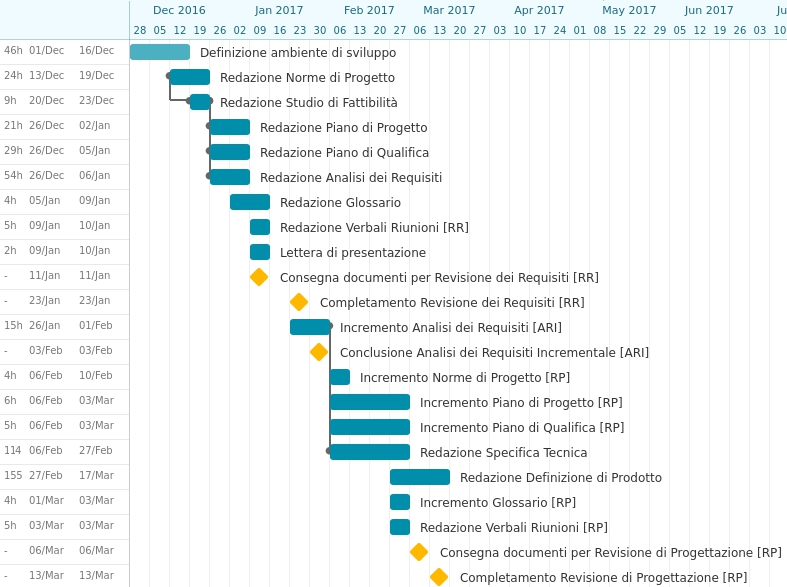
\includegraphics[width=1.2\textwidth]{img/ganttweeks1.png}}
\label{tab:genweeks}
\caption{\gloss{Diagramma di Gantt} della pianificazione generale, in settimane (parte 1)}

Nota: la "dipendenza all'indietro" che sembra esistere tra \emph{Redazione Norme di Progetto} e \emph{Redazione Studio di Fattibilità} non esiste (vedi prossimi diagrammi in giorni).
\end{figure}


\begin{figure}[H]
\makebox[\textwidth][c]{
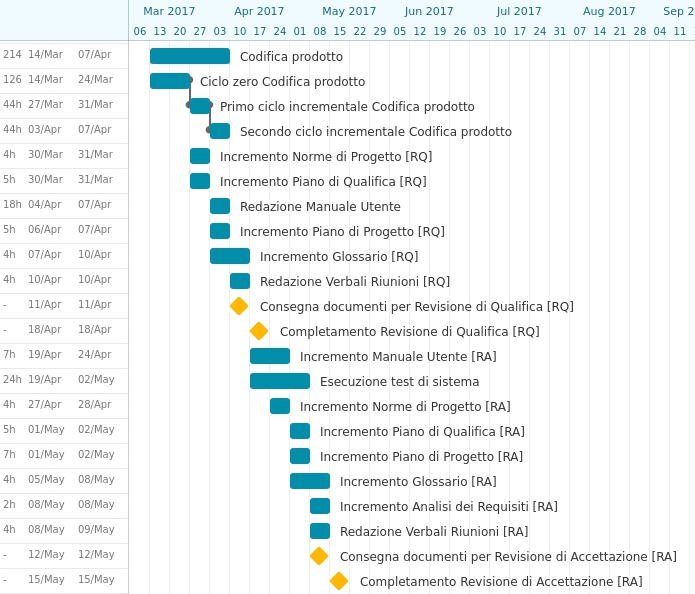
\includegraphics[width=1.2\textwidth]{img/ganttweeks2.png}}
\label{tab:genweeks}
\caption{Diagramma di Gantt della pianificazione generale, in settimane (parte 2)}
\end{figure}




\subsection{Suddivisione delle Attività}
	\subsubsection{\AR} \label{sec:AR}
	\textbf{Periodo}: dal 29-11-2016 al 11-01-2017.
	\\ Questo periodo inizia successivamente alla formazione del gruppo e finisce in corrispondenza della consegna dei documenti per la \emph{Revisione dei Requisiti}.
	Questo periodo prevede che siano stilati i seguenti documenti:
	\begin{description}
		\item[Norme di Progetto] in questo documento sono inserite tutte le norme che il team dovrà seguire e rispettare durante l'intero svolgimento delle attività. Tale documento è redatto dall'\AMx{}, mentre il \Vx{} ha il compito di certificare che tali norme siano state rispettate da tutto il gruppo;
		\item[Studio di Fattibilità] in questo documento sono analizzati i vari capitolati proposti. Per ogni capitolato, è stato analizzato il dominio applicativo/tecnologico e sono state inserite delle considerazioni in merito agli aspetti positivi e negativi;
		\item[Analisi dei requisiti] in questo documento sono raccolti tutti i requisiti progettuali necessari per comprendere più approfonditamente	il capitolato scelto con lo \emph{Studio di Fattibilità};
		\item[Piano di Progetto] questo documento è redatto dal \emph{Responsibile di Progetto} che organizza tutte le attività e stima le risorse, costi e tempi necessari per lo svolgimento del progetto;
		\item[Piano di Qualifica] questo documento è redatto dal \Vx{} che individua tutte le strategie di verifica e validazione che il team deve adottare per il progetto per ottenere e consegnare un prodotto di qualità;
		\item[Glossario] questo documento è steso da tutti i redattori in parallelo alla stesura degli altri documenti; esso contiene la spiegazione di alcuni termini presenti nei vari documenti al fine di chiarire il significato del termine stesso;
		\item[Lettera di presentazione] questo documento viene presentato al committente al fine di mostrare l'interesse del gruppo di partecipare alla gara d'appalto.
	\end{description}
	
	
\pagebreak
\begin{figure}[H]
\makebox[\textwidth][c]{
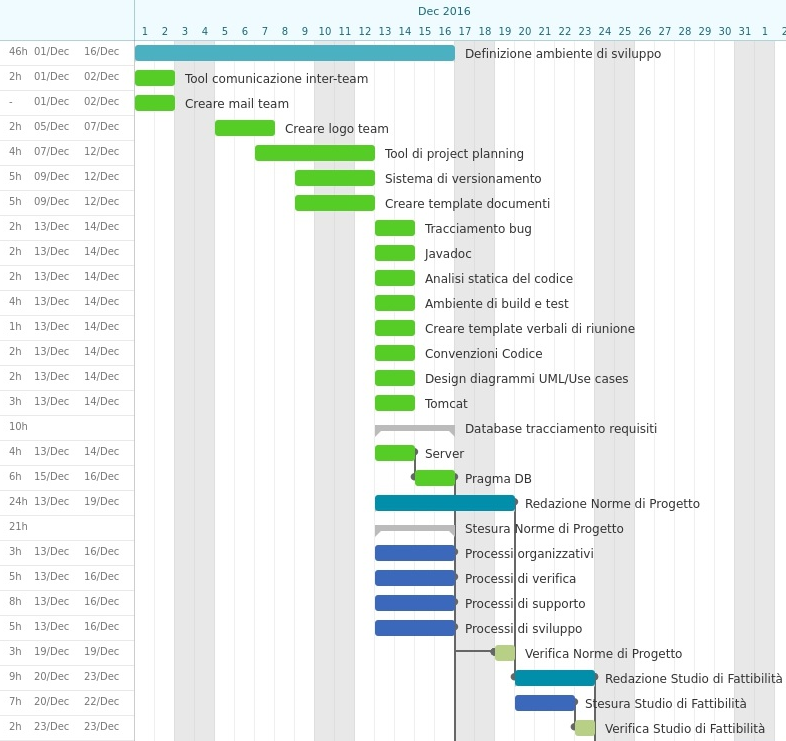
\includegraphics[width=1.2\textwidth]{img/ganttan1.png}}
\label{img:genweeks1}
\caption{Diagramma di Gantt della pianificazione dell'\AR, in giorni (parte 1)}
\end{figure}

\pagebreak
\begin{figure}[H]
\makebox[\textwidth][c]{
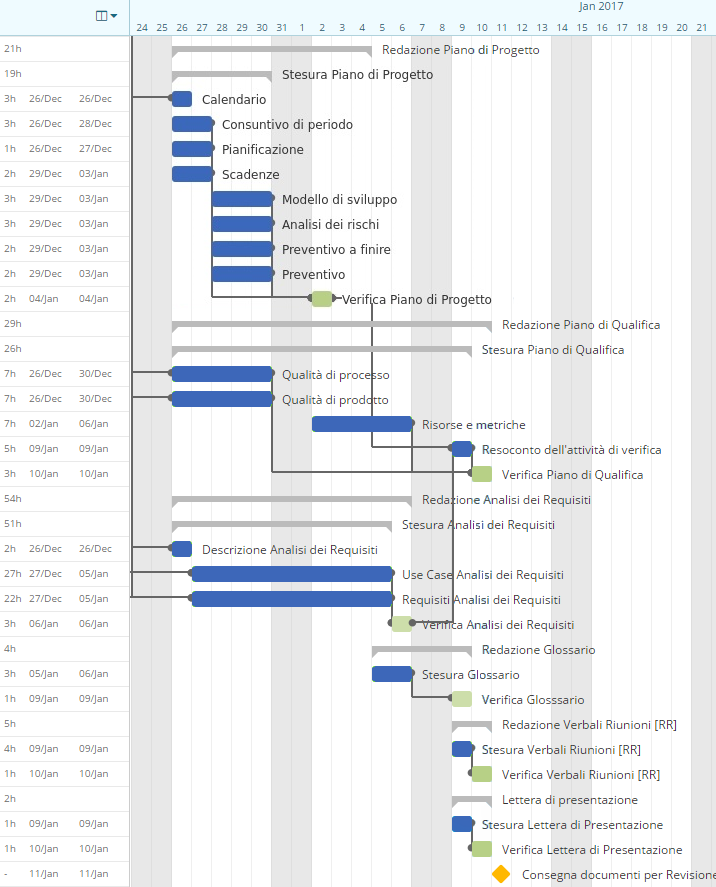
\includegraphics[width=1.0\textwidth]{img/ganttan21.png}}
\label{tab:genweeks2}
\caption{Diagramma di Gantt della pianificazione dell'\AR, in giorni (parte 2)}

Note:
\begin{itemize}
	\item l'attività \emph{Redazione Analisi dei Requisiti} ha una dipendenza verso l'attività PragmaDB appartenente all'attività \emph{Database tracciamento requisiti};
	\item le attività \emph{Redazione Piano di Progetto}, \emph{Redazione Piano di Qualifica} e \emph{Redazione Analisi dei Requisiti} hanno una dipendenza verso l'attività \emph{Redazione Studio di Fattibilità}.
	\item l'attività \emph{Resoconto dell'attività di verifica} richiede il completamento delle attività di verifica dell'\emph{Analisi dei Requisiti} e del \emph{Piano di Progetto}.
\end{itemize} 
\end{figure}
		
	\subsubsection{\ARI} \label{sec:ARI}
	\textbf{Periodo}: dal 24-01-2017 al 03-02-2017.
	\\ Questo periodo inizia in concomitanza con la \emph{Revisione dei Requisiti} e termina con una milestone interna che corrisponde all'inizio della \PA. In questo periodo, il gruppo mira ad integrare la documentazione precedentemente prodotta (in modo particolare l'\AR), con le correzioni suggerite durante la \emph{Revisione dei Requisiti} ed ampliarla tramite la definizione di alcuni requisiti opzionali.



\begin{figure}[H]
\makebox[\textwidth][c]{
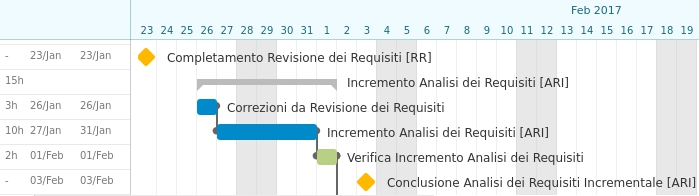
\includegraphics[width=1.2\textwidth]{img/ganttari.png}}
\label{tab:genweeks}
\caption{Diagramma di Gantt della pianificazione dell'\ARI, in giorni}
\end{figure}

	
	\subsubsection{\PA} \label{sec:PA}
	\textbf{Periodo}: dal 06-02-2017 al 06-03-2017.	
	\\ Questo periodo inizia subito dopo \ARI{} e si conclude con la consegna dei documenti per la \emph{Revisione di Progettazione}. La \PA{} prevede la stesura della progettazione ad alto livello e prevede lo svolgimento delle seguenti attività:
	\begin{description}
		\item[Incremento dei Documenti] in questa attività sono incrementati tutti i documenti della \PA{};
		\item[Redazione Specifica Tecnica] in questa attività sono descritte nel documento le scelte progettuali ad alto livello che il prodotto dovrà rispettare.
	\end{description}
	

\begin{figure}[H]
\makebox[\textwidth][c]{
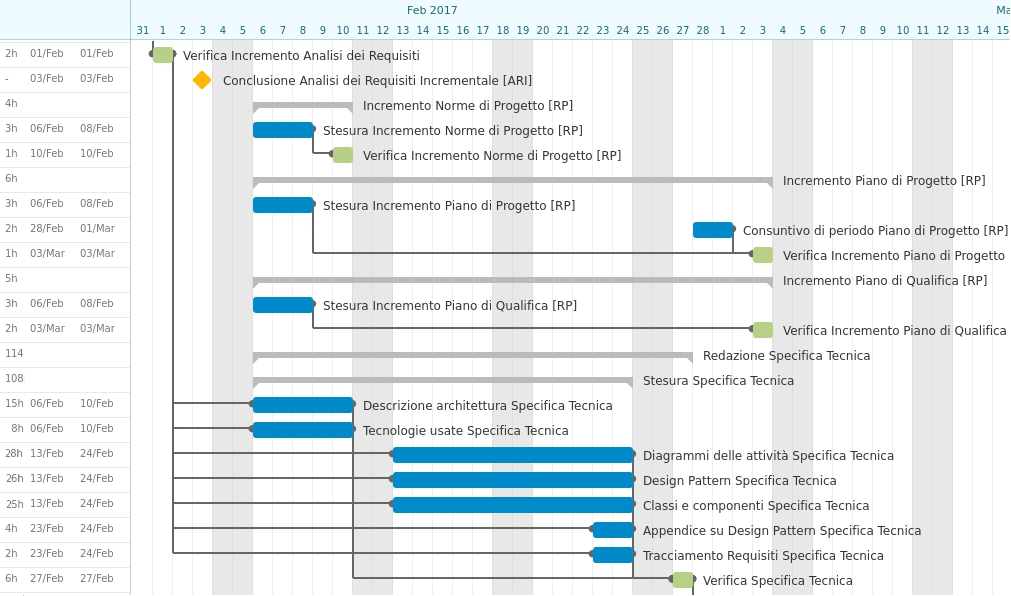
\includegraphics[width=1.2\textwidth]{img/ganttpa1.png}}
\label{tab:ganttpa1}
\caption{Diagramma di Gantt della pianificazione della \PA, in giorni (parte 1)}
\end{figure}

\begin{figure}[H]
\makebox[\textwidth][c]{
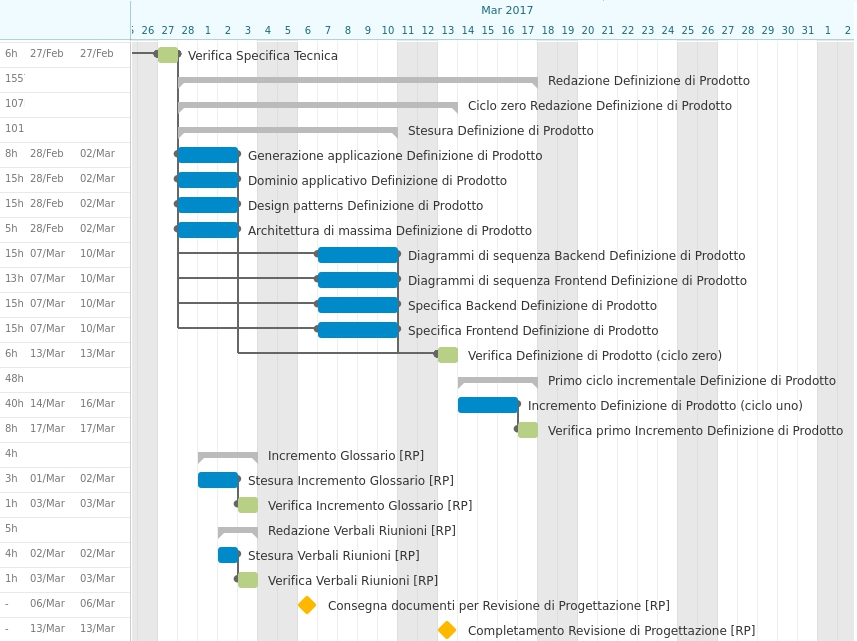
\includegraphics[width=1.2\textwidth]{img/ganttpa2.png}}
\label{tab:ganttpa2}
\caption{Diagramma di Gantt della pianificazione della \PA, in giorni (parte 2)}

Note:
\begin{itemize}
	\item Per raggiungere il completamento del perido successivo in tempo per la \emph{Revisione di Qualifica} si prevede di usare parte del tempo prima della scadenza del 06-03-2017 per la stesura della \emph{Definizione di Prodotto}.
\end{itemize} 
\end{figure}


	\subsubsection{\PDC} \label{sec:PDC}
	\textbf{Periodo}: dal 06-03-2017 al 11-04-2017.	
	\\ Questo periodo inizia subito dopo la \PA{} e si conclude con la consegna dei documenti per la \emph{Revisione di Qualifica}. La \PDC{} prevede la stesura della \emph{Definizione di Prodotto} e successivamente sarà avviata la fase di codifica. Le attività da svolgere sono le seguenti:
	\begin{description}
		\item[Incremento dei Documenti] in questa attività sono incrementati tutti i documenti basandosi sui risultati della \emph{Revisione di Progettazione}; 
		\item[Definizione di Prodotto] in questa attività è stilato questo documento che contiene la struttura e la relazione tra i vari componenti del prodotto, in base a quanto riportato nel documento \emph{Specifica Tecnica};
		\item[Codifica] in questa attività si procede allo sviluppo del codice del software da parte dei \emph{Programmatori}, attenendosi a quanto è riportato nella \emph{Definizione di Prodotto}; 
		\item[Redazione Manuale Utente] in questa attività si crea il documento destinato all'utente finale, che ha lo scopo di fornire le linee guida per il corretto utilizzo del software. Inoltre si crea il manuale utente sviluppatore, mirato a chiunque desideri ampliare il software già esistente.
	\end{description}
	
\begin{figure}[H]
\makebox[\textwidth][c]{
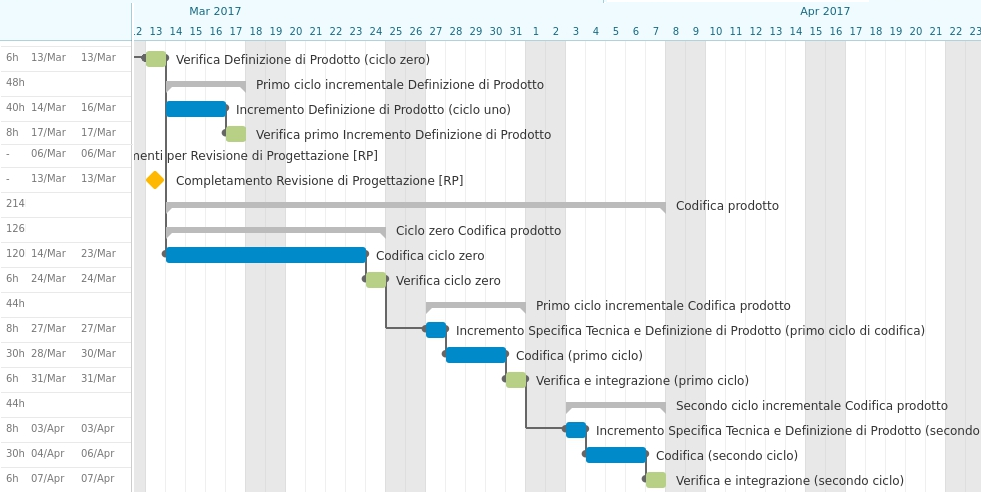
\includegraphics[width=1.2\textwidth]{img/ganttpdc1.png}}
\label{tab:ganttpa1}
\caption{Diagramma di Gantt della pianificazione della \PDC, in giorni (parte 1)}
\end{figure}

\begin{figure}[H]
\makebox[\textwidth][c]{
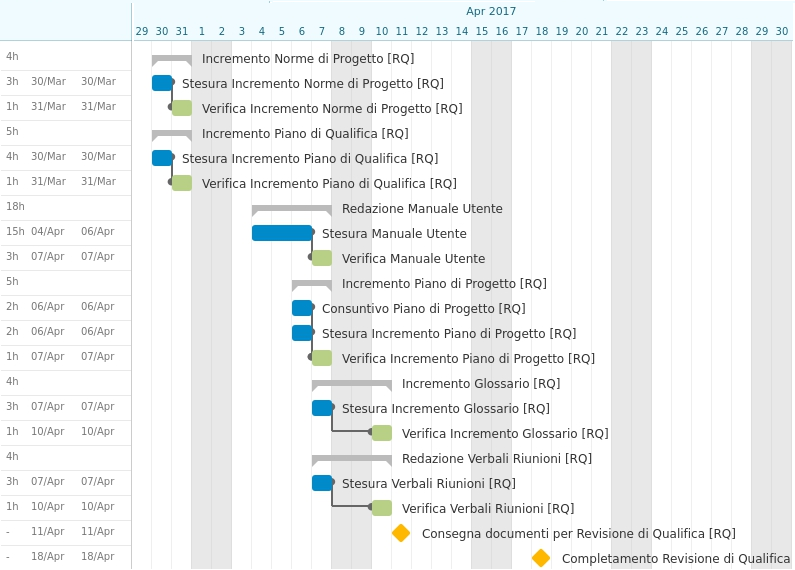
\includegraphics[width=1.2\textwidth]{img/ganttpdc2.png}}
\label{tab:ganttpa1}
\caption{Diagramma di Gantt della pianificazione della \PDC, in giorni (parte 2)}
\end{figure}


	\subsubsection{Verifica e Validazione} \label{sec:VV}

	\subsubsection{\VV} \label{sec:VV}
	\textbf{Periodo}: dal 18-04-2017 al 14-05-2017.
	\\ Questo periodo inizia subito dopo la \PDC{} e si conclude con la consegna del prodotto finale alla \emph{Revisione di Accettazione}. In questo periodo vengono effettuati i test del software, atti a garantire un prodotto finale che soddisfi i requisiti contenuti nell'\AR. Le attività da svolgere sono:
	\begin{description}
		\item[Test] effettuare dei test per il collaudo del sistema;
		\item[Incremento e Verifica dei Documenti] in questa attività verranno incrementati verificati tutti i documenti, basandosi sui risultati della \emph{Revisione di Qualifica}.
	\end{description}		
	
\begin{figure}[H]
\makebox[\textwidth][c]{
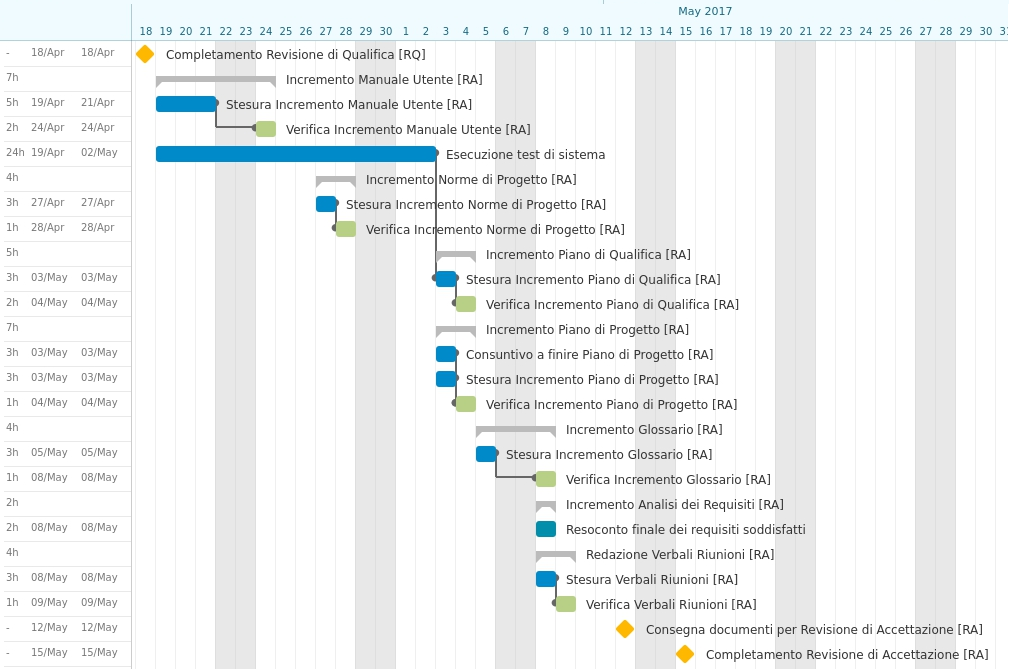
\includegraphics[width=1.2\textwidth]{img/ganttva.png}}
\label{tab:ganttpa1}
\caption{Diagramma di Gantt della pianificazione della \VV, in giorni}
\end{figure}





%%%%%%%%%%%%%%%%%%%%%%%%%%%%%%%%%%%%%
%%  Suddivisione delle ore lavorative
%%%%%%%%%%%%%%%%%%%%%%%%%%%%%%%%%%%%%
	
\section{Suddivisione delle ore lavorative e preventivo} \label{sec:preventivo}

Di seguito è riportata la pianificazione di dettaglio delle attività, suddivisa nei periodi descritti precedentemente. Per ogni periodo, sono presenti una tabella e dei grafici che descrivono e rappresentano i ruoli assunti da ciascun componente, il relativo quantitativo di ore impiegato e la rispettiva retribuzione.
A conclusione, è illustrato un quadro riassuntivo.

\newcommand{\roww}[7]{
	#1 & #2 & #3 & #4 & #5 & #6 & #7
}

\newcommand{\x}[7]{
	\begin{figure}[h]
		\begin{tabular}{ | l | c | c | c | c | c | c | r   }
			\hline
			Ruolo / persona & \R & \AM & \AN & \PJ & \PG & \V & Totale ore per persona \\ \hline
			\PB & \roww[#1] \\ \hline
			\LB & \roww[#2] \\ \hline
			\GG & \roww[#3] \\ \hline
			\MM & \roww[#4] \\ \hline
			\LS & \roww[#5] \\ \hline
			\AZ & \roww[#6] \\ \hline
			Totale ore per ruolo & \roww[#7] \\ \hline
		\end{tabular}
	\end{figure}
}

\newcommand{\intropreventivo}[1]{
	Di seguito si riporta la divisione oraria pianificata nella fase di #1.

	Successivamente sono evidenziate graficamente la divisione delle ore per persona e per ruolo. 
}

\newcommand{\introcosto}[1]{
	Di seguito si riporta il costo della #1.
}

\pagebreak[4]
\subsection{\AR}

\intropreventivo{\AR}
% i colori danno problemi di visualizzazione alle linee
\begin{figure}[H]
\makebox[\textwidth][c]
{
\definecolor{white2}{rgb}{0.95,0.95,0.95}
\definecolor{white3}{rgb}{0.9,0.9,0.9}
%\rowcolors{1}{white}{white2}

  \begin{tabular}{ | l | c | c | c | c | c | c | r |}
    \hline
    \rowcolor[gray]{.9}
    Ruolo / persona & \R & \AM & \AN & \PJ & \PG & \V & Tot ore/persona \\ \hline
    \PB & 7 & 3 & 14 & 0 & 0 & 7 & 31 \\ \hline
    \LB & 12 & 11 & 6 & 0 & 0 & 6 & 35 \\ \hline
    \GG & 0 & 24 & 8 & 0 & 0 & 3 & 35 \\ \hline
    \MM & 0 & 20 & 8 & 0 & 0 & 4 & 32\\ \hline
    \LS & 0 & 2 & 12 & 0 & 0 & 17 & 31\\ \hline
    \AZ & 1 & 4 & 13 & 0 & 0 & 12 & 30 \\ \hline
    \rowcolor[gray]{.9}

    Totale ore/ruolo & 20 & 64 & 61 & 0 & 0 & 49 & 194 \\ \hline
    
  \end{tabular}
}
\caption{Ore/ruolo per persona durante l'\AR.}

%\vspace*{1 cm}
\end{figure}

\pagebreak


\begin{figure}[H]
\makebox[\textwidth][c]
{
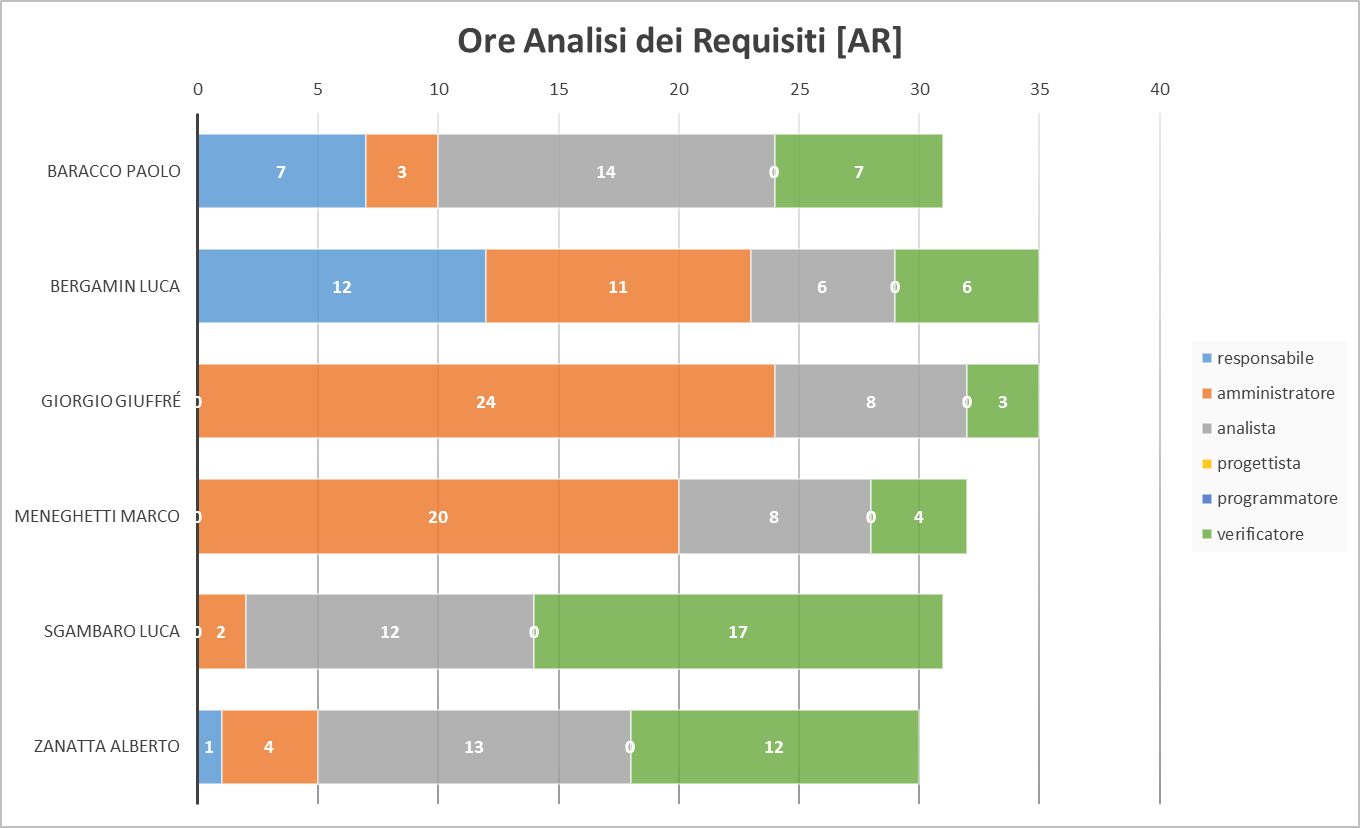
\includegraphics[width=1.1\textwidth]{img/orear1.png}
}
\caption{Ore/ruolo per persona durante l\AR.}
\label{fig:ar1}

\end{figure}

\begin{figure}[H]
\makebox[\textwidth][c]{
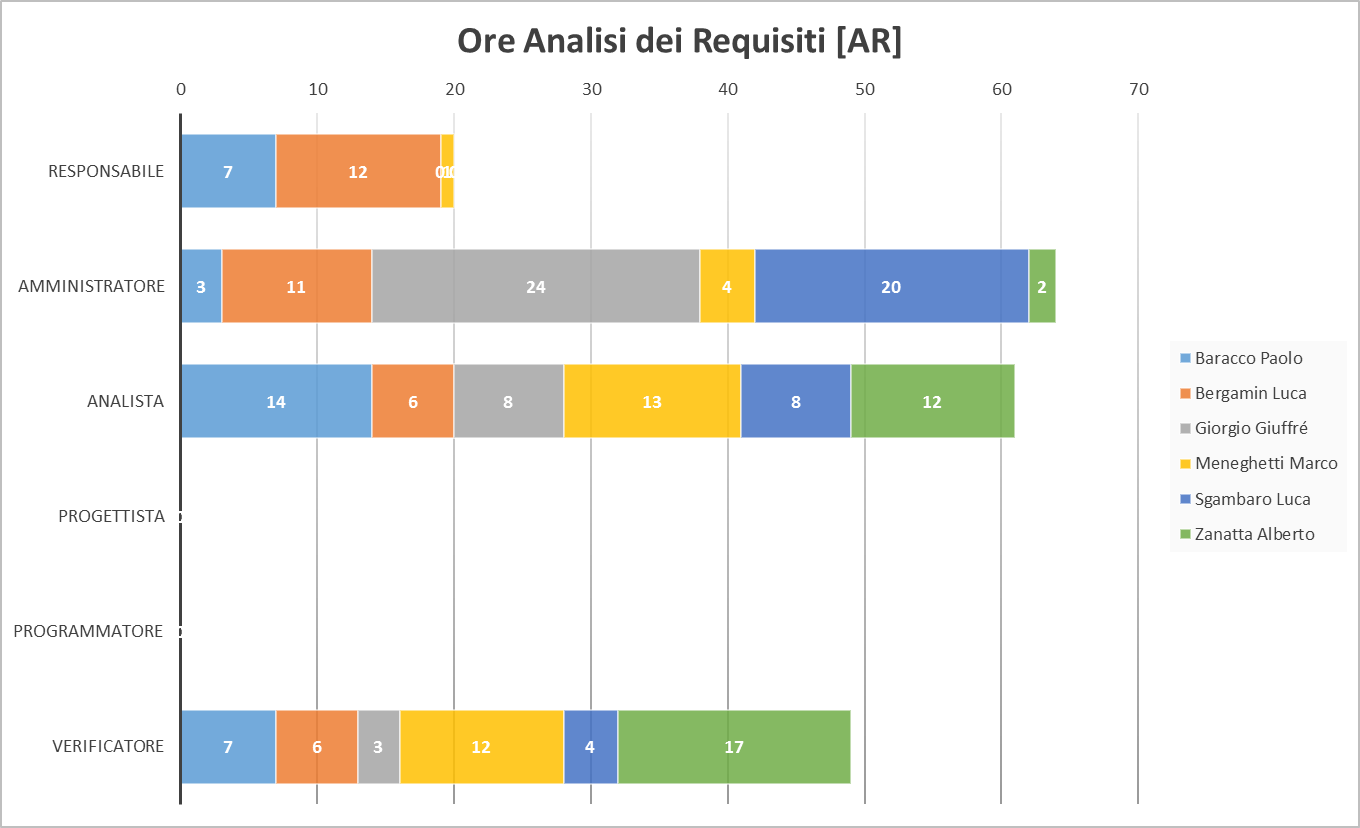
\includegraphics[width=1.1\textwidth]{img/orear2.png}\par
}
\caption{Ore/persona per ruolo durante l'\AR.}
\label{fig:ar2}
\end{figure}
	
\pagebreak
\subsubsection{Costo \AR}
	
\introcosto{\AR}
Questo costo viene fornito a scopo informativo e rappresenta l'investimento effettuato da \hx{} prima dell'aggiudicazione dell'appalto e perciò tale periodo \textbf{non è a carico del cliente}. 

Gli sforzi maggiori si evidenziano nel ruolo di:
\begin{itemize}
\item {\AMx} a causa dell'impegno aggiuntivo dedicato alla creazione di un proprio \emph{way of working};
\item {\ANx} per gli sforzi impiegati a raggiungere una comprensione profonda dei requisiti del progetto affrontato.
\end{itemize}

\begin{figure}[H]
\makebox[\textwidth][c]
{
\definecolor{white2}{rgb}{0.95,0.95,0.95}
\definecolor{white3}{rgb}{0.9,0.9,0.9}
%\rowcolors{1}{white}{white2}

  \begin{tabular}{ | l | c | c | c | c | c | c | r |}
    \hline
    \rowcolor[gray]{.9}
    Ruolo / persona & \R & \AM & \AN & \PJ & \PG & \V & Tot euro/persona \\ \hline
    \PB & 210 & 60 & 350 & 0 & 0 & 105 & 725 \\ \hline
    \LB & 360 & 220 & 150 & 0 & 0 & 90 & 820 \\ \hline
    \GG & 0 & 480 & 200 & 0 & 0 & 45 & 725 \\ \hline
    \MM & 0 & 400 & 200 & 0 & 0 & 60 & 660 \\ \hline
    \LS & 0 & 40 & 300 & 0 & 0 & 255 & 595 \\ \hline
    \AZ & 30 & 80 & 325 & 0 & 0 & 180 & 615 \\ \hline
    \rowcolor[gray]{.9}

    Totale euro/ruolo & 600 & 1280 & 1525 & 0 & 0 & 735 & 4140 \\ \hline
  \end{tabular}
  
}\label{tab:car}

  \caption{Tabella costo {\AR} per ruolo e per persona, valori in euro (\euro).}
\end{figure}

\begin{figure}[H]
\makebox[\textwidth][c]{
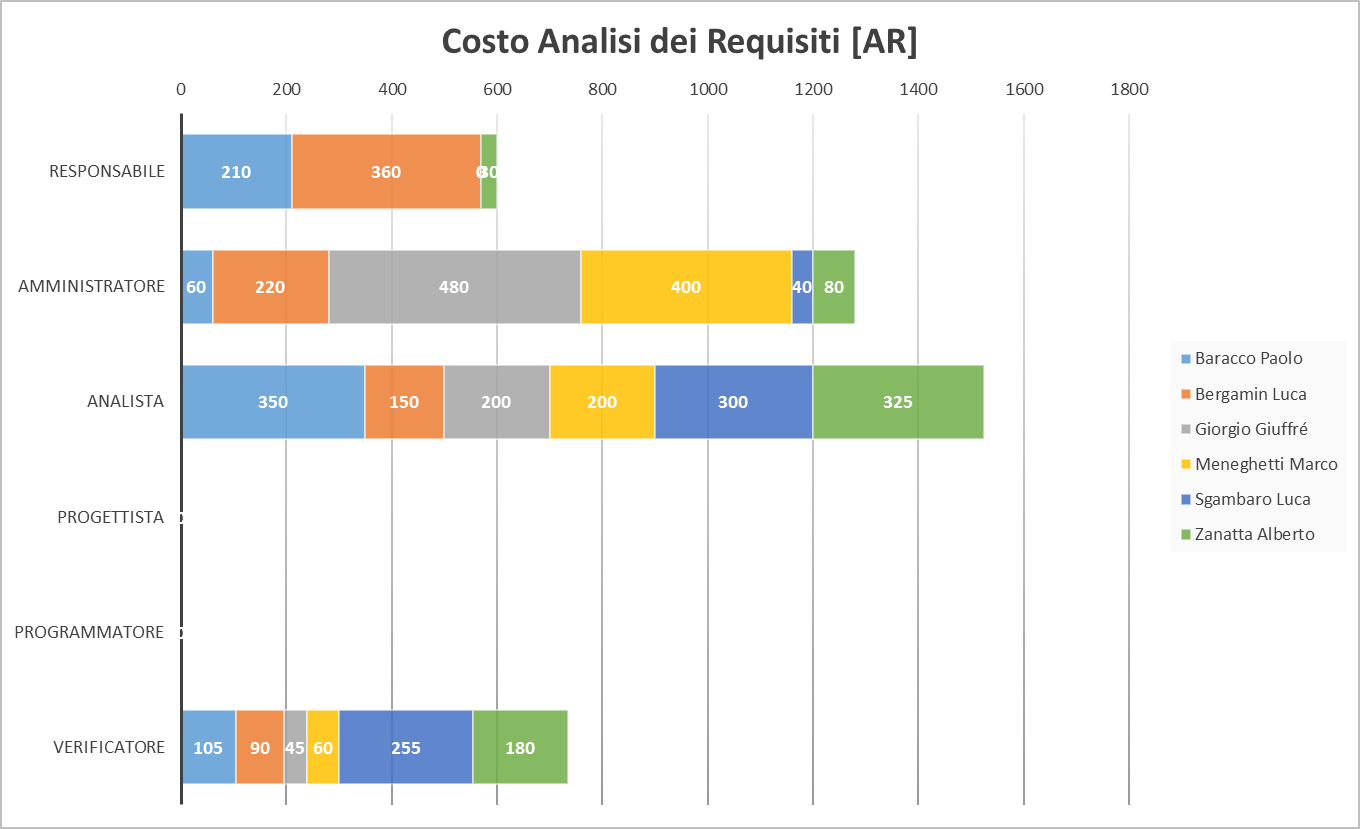
\includegraphics[width=1.05\textwidth]{img/costoar.png}\par
}
\caption{Costo {\AR} per ruolo, valori in euro (\euro).}
\label{fig:car}
\end{figure}



%\x
%{\roww{7}{3}{14}{0}{0}{7}{31}}
%{\roww{12}{11}{6}{0}{0}{6}{35}}
%{\roww{0}{24}{8}{0}{0}{3}{35}}
%{\roww{0}{20}{8}{0}{0}{4}{32}}
%{\roww{0}{2}{12}{0}{0}{17}{31}}
%{\roww{1}{4}{13}{0}{0}{12}{30}}
%{\roww{20}{64}{61}{0}{0}{49}{194}}


\pagebreak[4]
\subsection{\ARI}
\intropreventivo{\ARI}


\begin{figure}[H]

\makebox[\textwidth][c]
{
\definecolor{white2}{rgb}{0.95,0.95,0.95}
\definecolor{white3}{rgb}{0.9,0.9,0.9}
%\rowcolors{1}{white}{white2}

  \begin{tabular}{ | l | c | c | c | c | c | c | r |}
    \hline
    \rowcolor[gray]{.9}
    Ruolo / persona & \R & \AM & \AN & \PJ & \PG & \V & Tot ore/persona \\ \hline
    \PB & 0 & 0 & 0 & 0 & 0 & 0 & 0 \\ \hline
    \LB & 0 & 0 & 0 & 0 & 0 & 0 & 0 \\ \hline
    \GG & 0 & 0 & 0 & 0 & 0 & 2 & 2 \\ \hline
    \MM & 0 & 0 & 0 & 0 & 0 & 0 & 0 \\ \hline
    \LS & 0 & 0 & 5 & 0 & 0 & 0 & 5 \\ \hline
    \AZ & 0 & 0 & 8 & 0 & 0 & 0 & 8 \\ \hline
    \rowcolor[gray]{.9}

    Totale ore/ruolo & 0 & 0 & 13 & 0 & 0 & 2 & 15 \\ \hline
    
  \end{tabular}
}
\caption{Ore/ruolo per persona durante l'\ARI.}

\end{figure} 
% i colori danno problemi di visualizzazione alle linee
\pagebreak


\begin{figure}[H]
\makebox[\textwidth][c]{
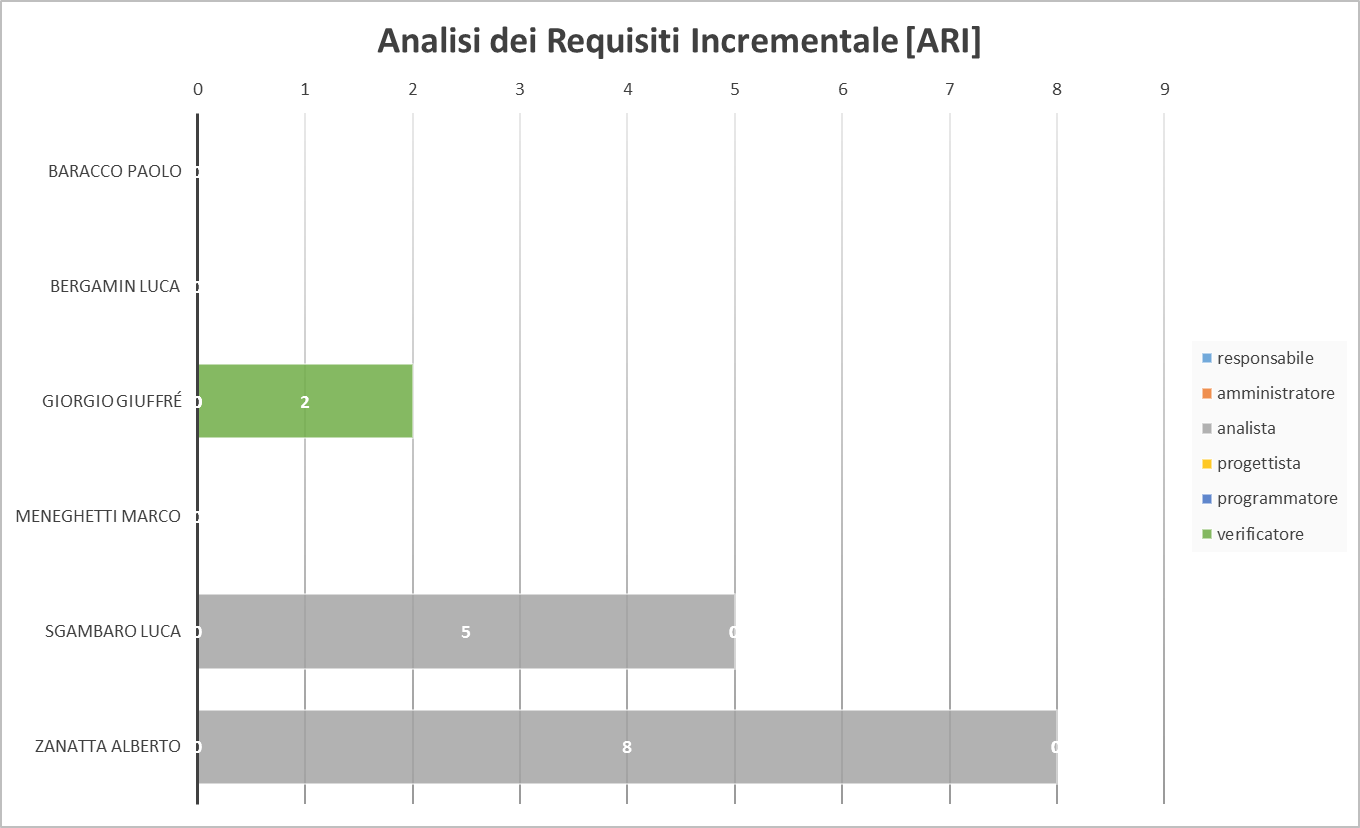
\includegraphics[width=1.15\textwidth]{img/oreari1.png}}
\caption{Ore/ruolo per persona durante l'\ARI.}
\label{fig:ari}

\end{figure}

\begin{figure}[H]
\makebox[\textwidth][c]{
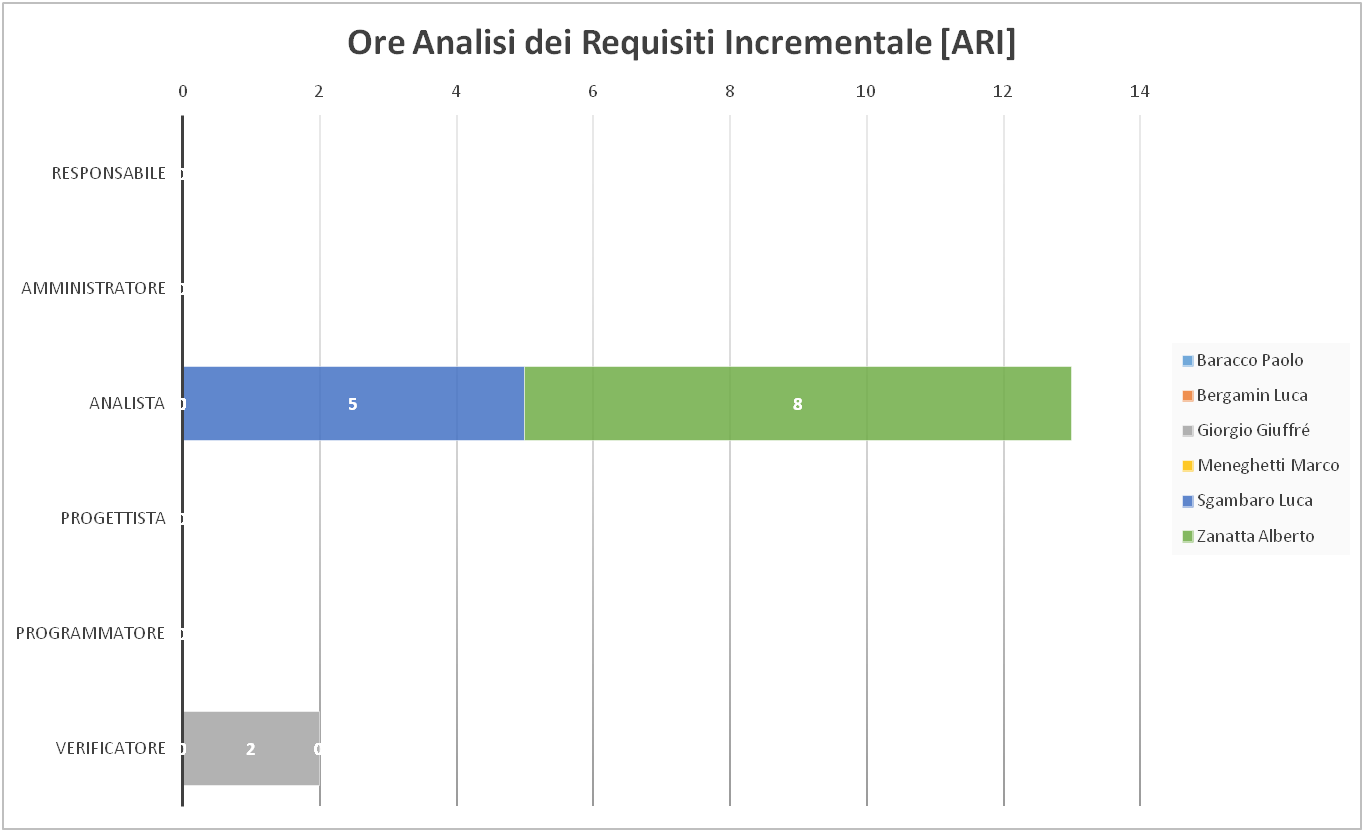
\includegraphics[width=1.15\textwidth]{img/oreari2.png}}
\caption{Ore/persona per ruolo durante l'\ARI.}
\label{fig:ari2}

\end{figure}

\pagebreak

\subsubsection{Costo \ARI}

\introcosto{\ARI}
Questo costo rappresenta gli sforzi che {\hx} affronterà al fine di consolidare la comprensione dei requisiti del progetto.

Tale periodo è ridotto rispetto a quanto desiderato in quanto coincidente con la sessione d'esami dell'Università degli Studi di Padova. % togliere?

Gli sforzi maggiori si evidenziano nel ruolo di:
\begin{itemize}
\item {\ANx} per gli sforzi impiegati a raggiungere una comprensione profonda dei requisiti del progetto affrontato.
\end{itemize}

\begin{figure}[H]
\makebox[\textwidth][c]
{
\definecolor{white2}{rgb}{0.95,0.95,0.95}
\definecolor{white3}{rgb}{0.9,0.9,0.9}
%\rowcolors{1}{white}{white2}

  \begin{tabular}{ | l | c | c | c | c | c | c | r |}
    \hline
    \rowcolor[gray]{.9}
    Ruolo / persona & \R & \AM & \AN & \PJ & \PG & \V & Tot euro/persona \\ \hline
    \PB & 0 & 0 & 0 & 0 & 0 & 0 & 0 \\ \hline
    \LB & 0 & 0 & 0 & 0 & 0 & 0 & 0 \\ \hline
    \GG & 0 & 0 & 0 & 0 & 0 & 30 & 30 \\ \hline
    \MM & 0 & 0 & 0 & 0 & 0 & 0 & 0 \\ \hline
    \LS & 0 & 0 & 125 & 0 & 0 & 0 & 125 \\ \hline
    \AZ & 0 & 0 & 200 & 0 & 0 & 0 & 200 \\ \hline
    \rowcolor[gray]{.9}

    Totale euro/ruolo & 0 & 0 & 325 & 0 & 0 & 30 & 355 \\ \hline
  \end{tabular}
  
}\label{tab:cari}

  \caption{Tabella costo {\ARI} per ruolo e per persona, valori in euro (\euro).}
\end{figure}

\begin{figure}[H]
\makebox[\textwidth][c]{
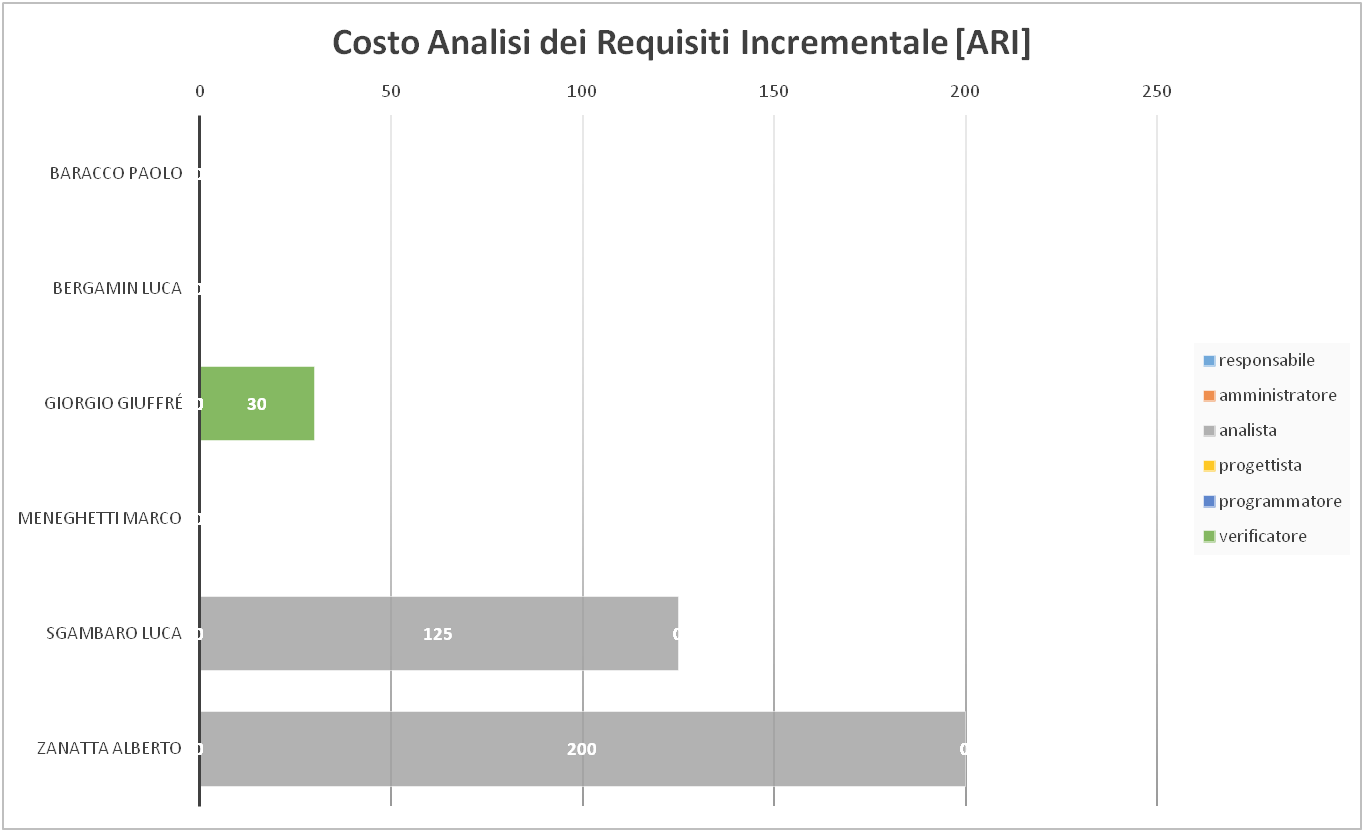
\includegraphics[width=1.2\textwidth]{img/costoari.png}
}
\caption{Costo {\ARI} per ruolo, valori in euro (\euro).}


\end{figure}

\pagebreak[4]

\subsection{\PA}
\intropreventivo{\PA}

\begin{figure}[H]
\definecolor{white2}{rgb}{0.95,0.95,0.95}
\definecolor{white3}{rgb}{0.9,0.9,0.9}
%\rowcolors{1}{white}{white2}

\makebox[\textwidth][c]
{
  \begin{tabular}{ | l | c | c | c | c | c | c | r |}
    \hline
    \rowcolor[gray]{.9}
    Ruolo / persona & \R & \AM & \AN & \PJ & \PG & \V & Tot ore/persona \\ \hline
    \PB & 0 & 0 & 0 & 26 & 0 & 6 & 32 \\ \hline
    \LB & 0 & 3 & 0 & 38 & 0 & 1 & 42 \\ \hline
    \GG & 3 & 0 & 0 & 35 & 0 & 1 & 39 \\ \hline
    \MM & 0 & 0 & 0 & 42 & 0 & 4 & 46 \\ \hline
    \LS & 2 & 0 & 0 & 36 & 0 & 6 & 44 \\ \hline
    \AZ & 0 & 0 & 0 & 31 & 0 & 4 & 35 \\ \hline
    \rowcolor[gray]{.9}

    Totale ore/ruolo & 5 & 3 & 0 & 208 & 0 & 22 & 238 \\ \hline
    
  \end{tabular}
}
\caption{Ore/ruolo per persona durante la \PA.}
\end{figure} 
% i colori danno problemi di visualizzazione alle linee
\pagebreak

\begin{figure}[H]
\makebox[\textwidth][c]{
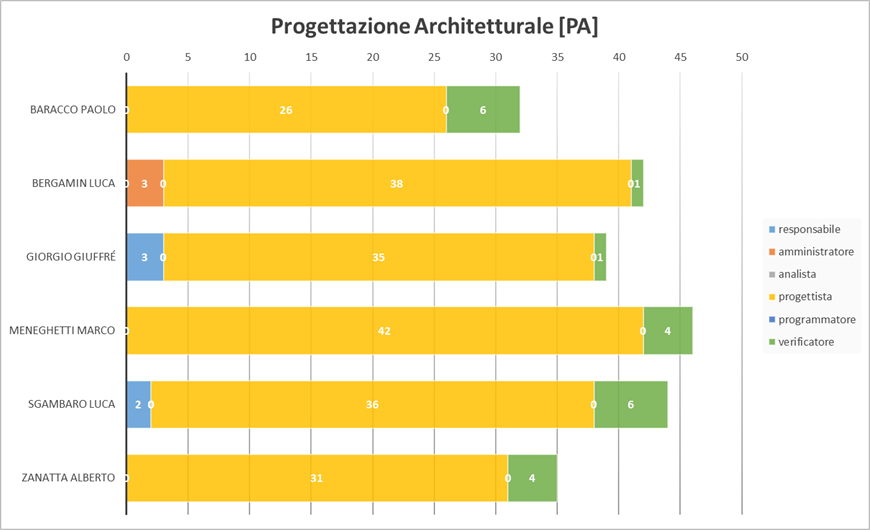
\includegraphics[width=1.1\textwidth]{img/orepa1.png}}
\caption{Ore/ruolo per persona durante la \PA.}
\label{fig:pa1}

\end{figure}

\begin{figure}[H]
\makebox[\textwidth][c]{
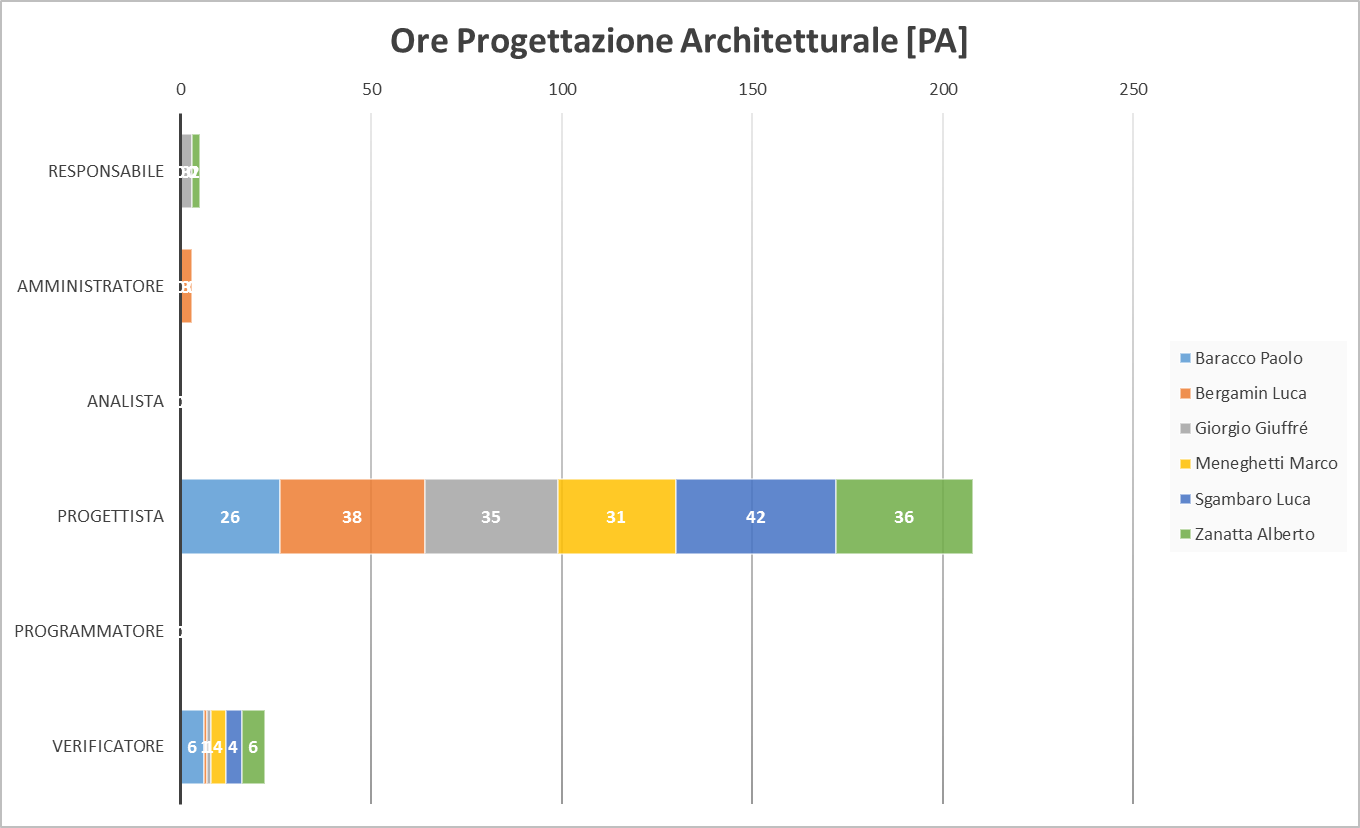
\includegraphics[width=1.1\textwidth]{img/orepa2.png}}
\caption{Ore/persona per ruolo durante la \PA.}
\label{fig:pa2}

\end{figure}

\pagebreak
\subsubsection{Costo \PA}
\introcosto{\PA}
Questa fase mira a consolidare la creazione di una solida base architetturale per \proj.

Gli sforzi maggiori si evidenziano nel ruolo di:
\begin{itemize}
\item {\PJx} per la creazione del documento di \emph{Specifica Tecnica} e parte del primo incremento della \emph{Definizione di Prodotto}.
\end{itemize}

\begin{figure}[H]
\makebox[\textwidth][c]
{
\definecolor{white2}{rgb}{0.95,0.95,0.95}
\definecolor{white3}{rgb}{0.9,0.9,0.9}
%\rowcolors{1}{white}{white2}

  \begin{tabular}{ | l | c | c | c | c | c | c | r |}
    \hline
    \rowcolor[gray]{.9}
    Ruolo / persona & \R & \AM & \AN & \PJ & \PG & \V & Tot euro/persona \\ \hline
    \PB & 0 & 0 & 0 & 572 & 0 & 90 & 662 \\ \hline
    \LB & 0 & 60 & 0 & 836 & 0 & 15 & 911 \\ \hline
    \GG & 90 & 0 & 0 & 770 & 0 & 15 & 875 \\ \hline
    \MM & 0 & 0 & 0 & 924 & 0 & 60 & 984 \\ \hline
    \LS & 60 & 0 & 0 & 792 & 0 & 90 & 942 \\ \hline
    \AZ & 0 & 0 & 0 & 682 & 0 & 60 & 742 \\ \hline
    \rowcolor[gray]{.9}

    Totale euro/ruolo & 150 & 60 & 0 & 4576 & 0 & 330 & 5116 \\ \hline
    
  \end{tabular}
  
}\label{tab:cpa}

  \caption{Tabella costo {\PA} per ruolo e per persona, valori in euro (\euro).}
\end{figure}

\begin{figure}[H]
\makebox[\textwidth][c]{
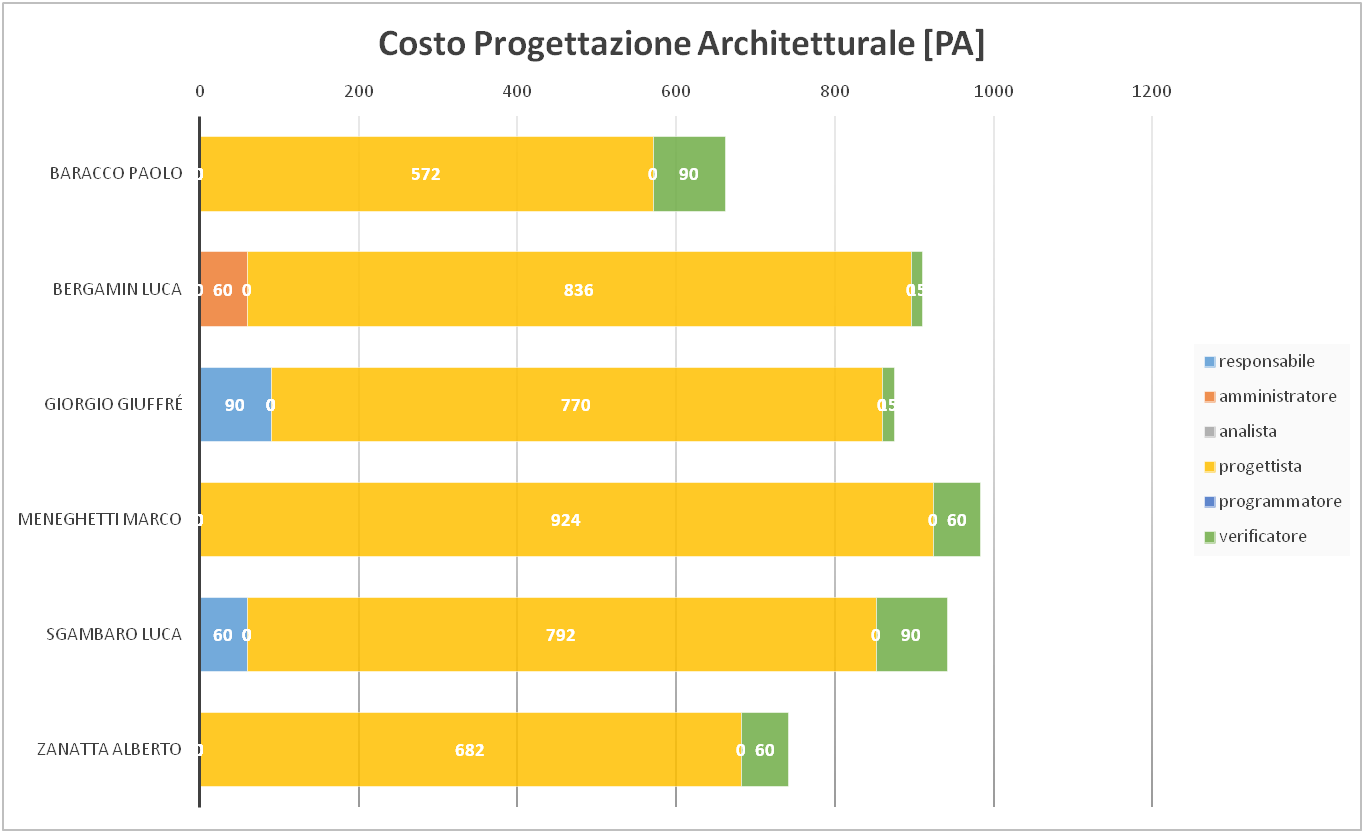
\includegraphics[width=1.2\textwidth]{img/costopa.png}}
  \caption{Costo \PA{} per ruolo e per persona, valori in euro (\euro).}
\end{figure}

\pagebreak[4]
\subsection{\PDC}
\intropreventivo{\PDC}

\begin{figure}[H]
\definecolor{white2}{rgb}{0.95,0.95,0.95}
\definecolor{white3}{rgb}{0.9,0.9,0.9}
%\rowcolors{1}{white}{white2}

\makebox[\textwidth][c]
{
  \begin{tabular}{ | l | c | c | c | c | c | c | r |}
    \hline
    \rowcolor[gray]{.9}
    Ruolo / persona & \R & \AM & \AN & \PJ & \PG & \V & Tot ore/persona \\ \hline
    \PB & 0 & 0 & 0 & 18 & 30 & 7 & 55 \\ \hline
    \LB & 0 & 5 & 0 & 8 & 30 & 13 & 56 \\ \hline
    \GG & 0 & 5 & 0 & 10 & 30 & 3 & 48 \\ \hline
    \MM & 2 & 0 & 0 & 0 & 30 & 8 & 40 \\ \hline
    \LS & 0 & 3 & 0 & 10 & 30 & 9 & 52 \\ \hline
    \AZ & 2 & 5 & 0 & 10 & 30 & 10 & 57 \\ \hline
    \rowcolor[gray]{.9}

    Totale ore/ruolo & 4 & 18 & 0 & 56 & 180 & 50 & 308 \\ \hline
    
  \end{tabular}
  }
    \caption{Ore/ruolo per persona durante la \PDC.}

\end{figure} 
% i colori danno problemi di visualizzazione alle linee

\pagebreak[4]

% USARE QUESTO PER IMMAGINI
\begin{figure}[H]
  \makebox[\textwidth][c]{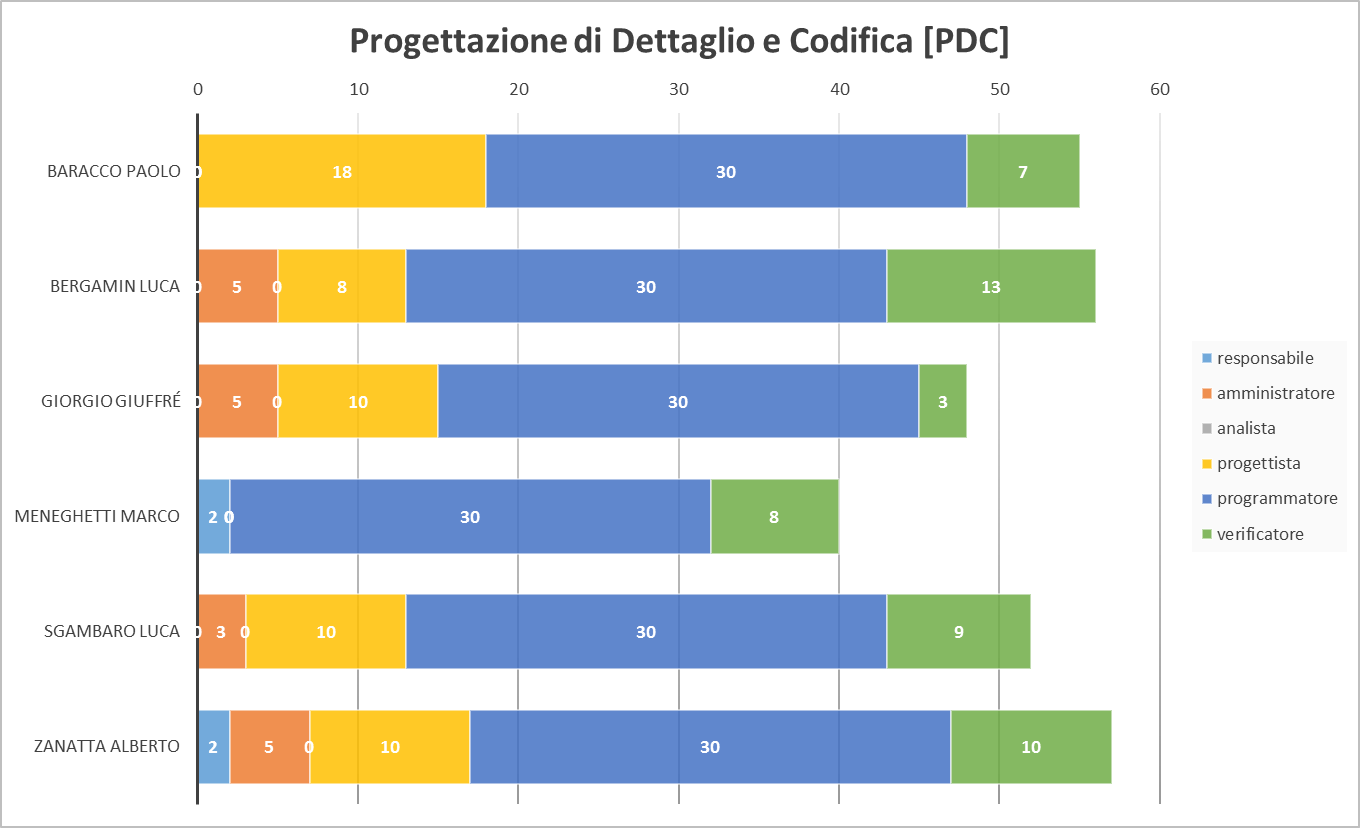
\includegraphics[width=1.1\textwidth]{img/orepdc1.png}}
  \caption{Ore/ruolo per persona durante la \PDC.}
\label{fig:pdc1}

\end{figure}



%	{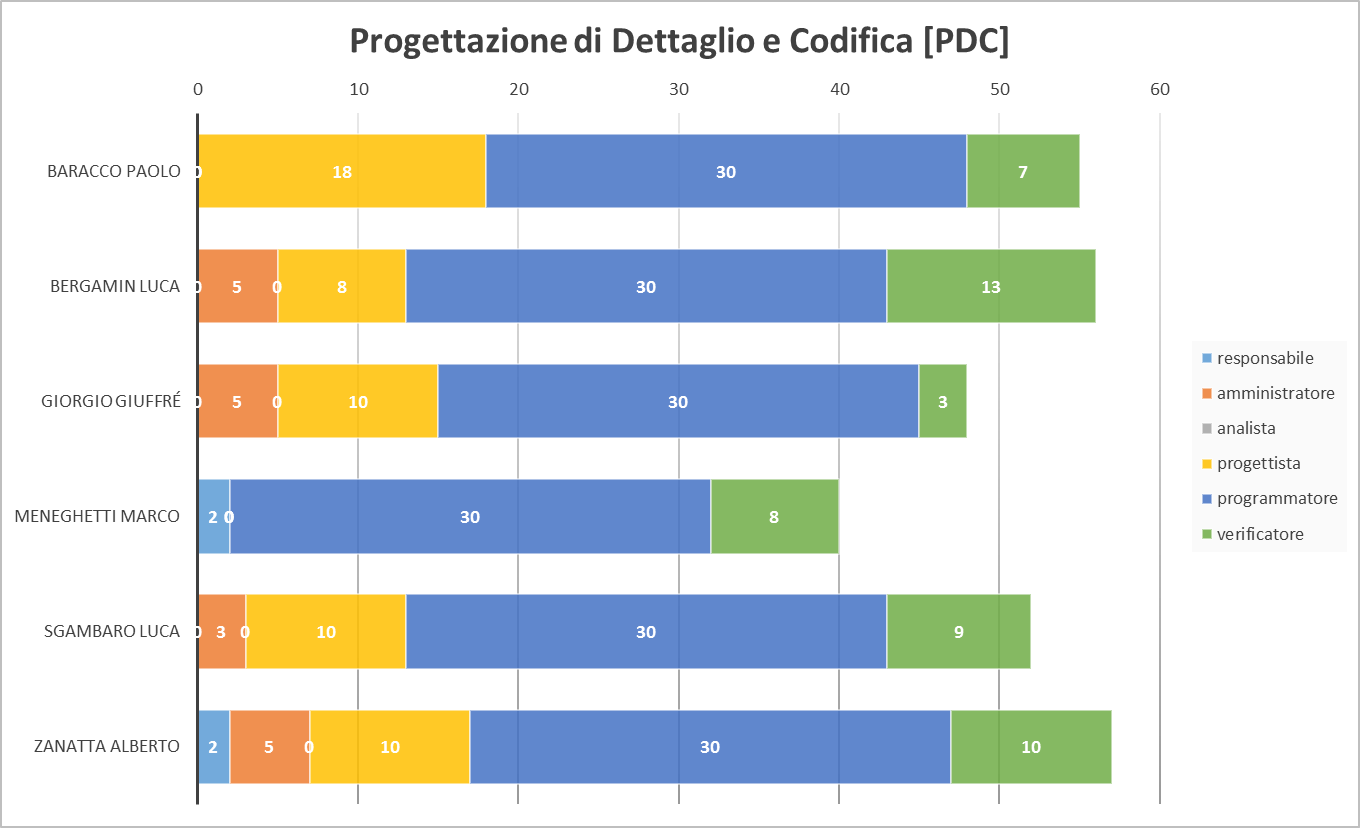
\includegraphics[width=15cm]{img/orepdc1.png}\par}

\begin{figure}[H]
\makebox[\textwidth][c]{
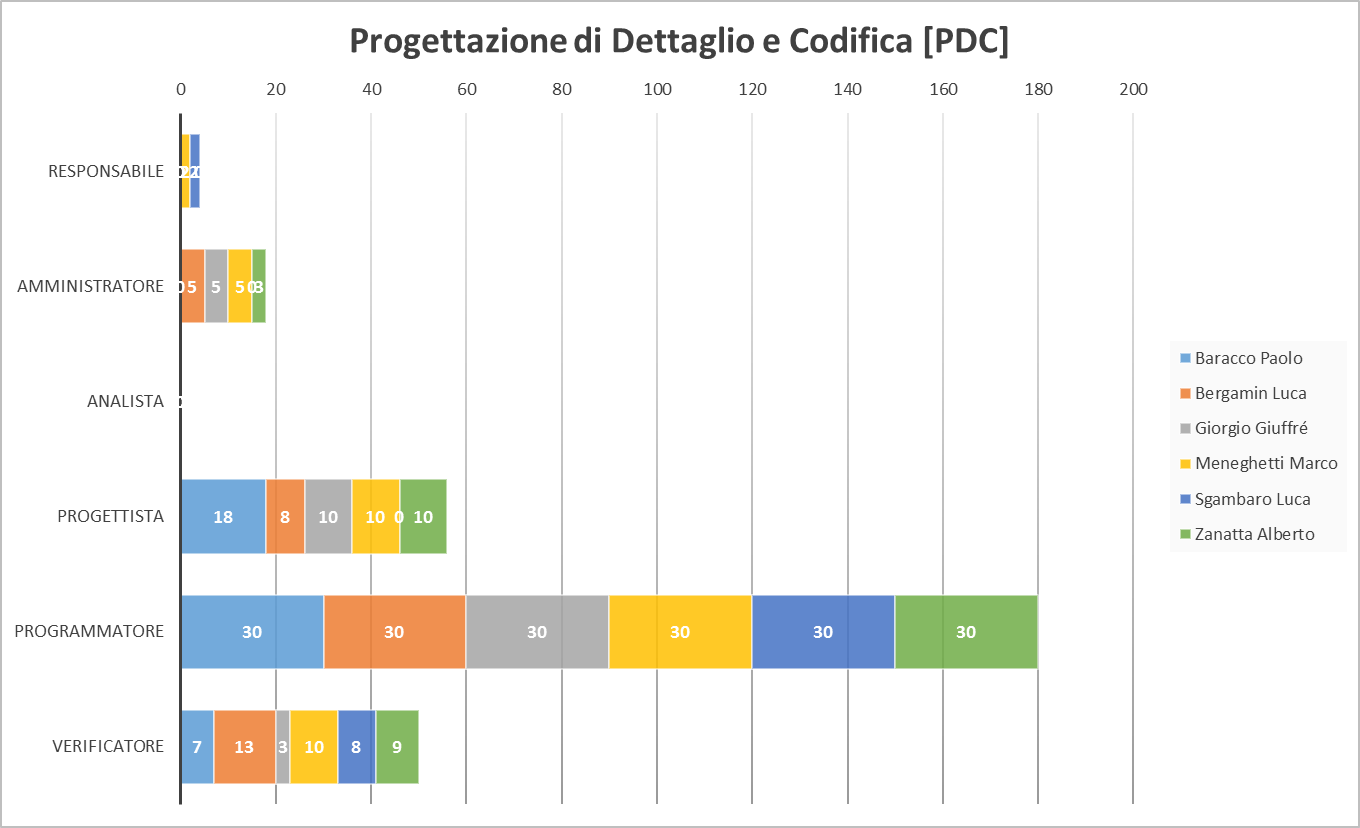
\includegraphics[width=1.1\textwidth]{img/orepdc2.png}}
\caption{Ore/persona per ruolo durante la \PDC.}
\label{fig:pdc2}

\end{figure}

\pagebreak
\subsubsection{Costo \PDC}
\introcosto{\PDC}
Questa fase mira a completare la \emph{Definizione di Prodotto} tramite incrementi e completare l'attività di codifica.

Gli sforzi maggiori si evidenziano nel ruolo di:
\begin{itemize}
\item {\PJx} per l'incremento della \emph{Definizione di Prodotto};
\item {\PGx} per l'attività di codifica;
\item {\Vx} per il controllo e la verifica del codice e dei documenti prodotti.
\end{itemize}

\begin{figure}[H]
\makebox[\textwidth][c]
{
\definecolor{white2}{rgb}{0.95,0.95,0.95}
\definecolor{white3}{rgb}{0.9,0.9,0.9}
%\rowcolors{1}{white}{white2}

  \begin{tabular}{ | l | c | c | c | c | c | c | r |}
    \hline
    \rowcolor[gray]{.9}
    Ruolo / persona & \R & \AM & \AN & \PJ & \PG & \V & Tot euro/persona \\ \hline
    \PB & 0 & 0 & 0 & 396 & 450 & 105 & 951 \\ \hline
    \LB & 0 & 100 & 0 & 176 & 450 & 195 & 921 \\ \hline
    \GG & 0 & 100 & 0 & 220 & 450 & 45 & 815 \\ \hline
    \MM & 60 & 0 & 0 & 0 & 450 & 120 & 630 \\ \hline
    \LS & 0 & 60 & 0 & 220 & 450 & 135 & 865 \\ \hline
    \AZ & 60 & 100 & 0 & 220 & 450 & 150 & 980 \\ \hline
    \rowcolor[gray]{.9}

    Totale euro/ruolo & 120 & 360 & 0 & 1232 & 2700 & 750 & 5162 \\ \hline
  \end{tabular}
  
}\label{tab:cpdc}

  \caption{Tabella costo {\PDC} per ruolo e per persona, valori in euro (\euro).}
\end{figure}
\begin{figure}[H]
\makebox[\textwidth][c]{
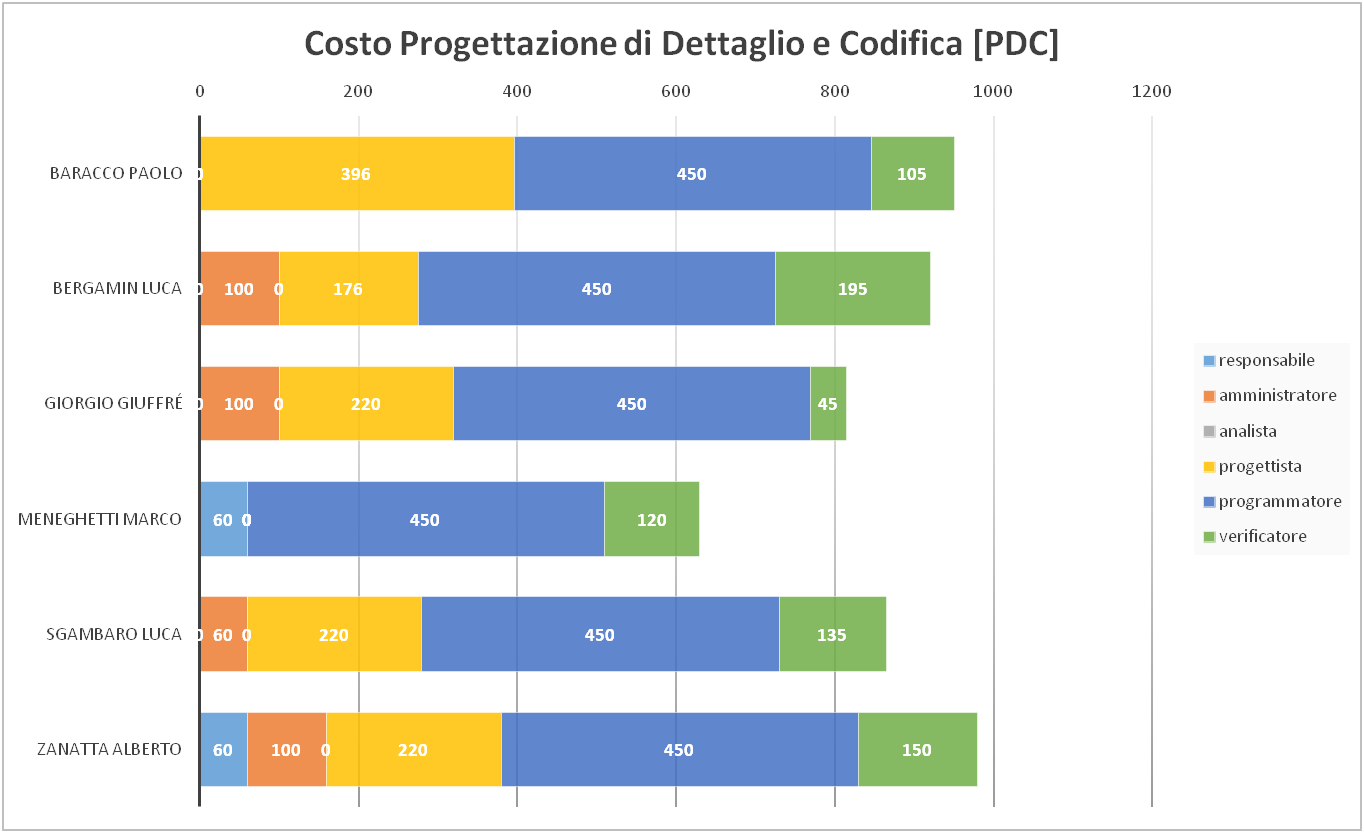
\includegraphics[width=1.2\textwidth]{img/costopdc.png}}
\label{tab:cpdc}

  \caption{Costo {\PDC} per ruolo, valori in euro (\euro).}
\end{figure}

\pagebreak[4]
\subsection{\VV}
\intropreventivo{\VV}

\begin{figure}[H]
\definecolor{white2}{rgb}{0.95,0.95,0.95}
\definecolor{white3}{rgb}{0.9,0.9,0.9}
%\rowcolors{1}{white}{white2}

\makebox[\textwidth][c]
{
  \begin{tabular}[width=1.2\textwidth]{ | l | c | c | c | c | c | c | r |}
    \hline
    \rowcolor[gray]{.9}
    Ruolo / persona & \R & \AM & \AN & \PJ & \PG & \V & Tot ore/persona \\ \hline
    \PB & 3 & 8 & 0 & 0 & 0 & 5 & 16 \\ \hline
    \LB & 3 & 0 & 0 & 0 & 0 & 2 & 5 \\ \hline
    \GG & 0 & 0 & 0 & 0 & 0 & 14 & 14 \\ \hline
    \MM & 0 & 0 & 2 & 0 & 0 & 15 & 17 \\ \hline
    \LS & 0 & 0 & 0 & 0 & 0 & 2 & 2 \\ \hline
    \AZ & 0 & 0 & 0 & 0 & 0 & 3 & 3 \\ \hline
    \rowcolor[gray]{.9}

    Totale ore/ruolo & 6 & 8 & 2 & 0 & 0 & 41 & 57 \\ \hline
    
  \end{tabular}
  }
  \caption{Ore/ruolo per persona durante la \VV.}
\label{fig:vv1}
\end{figure} 
% i colori danno problemi di visualizzazione alle linee

\pagebreak

\begin{figure}[H]
\makebox[\textwidth][c]{
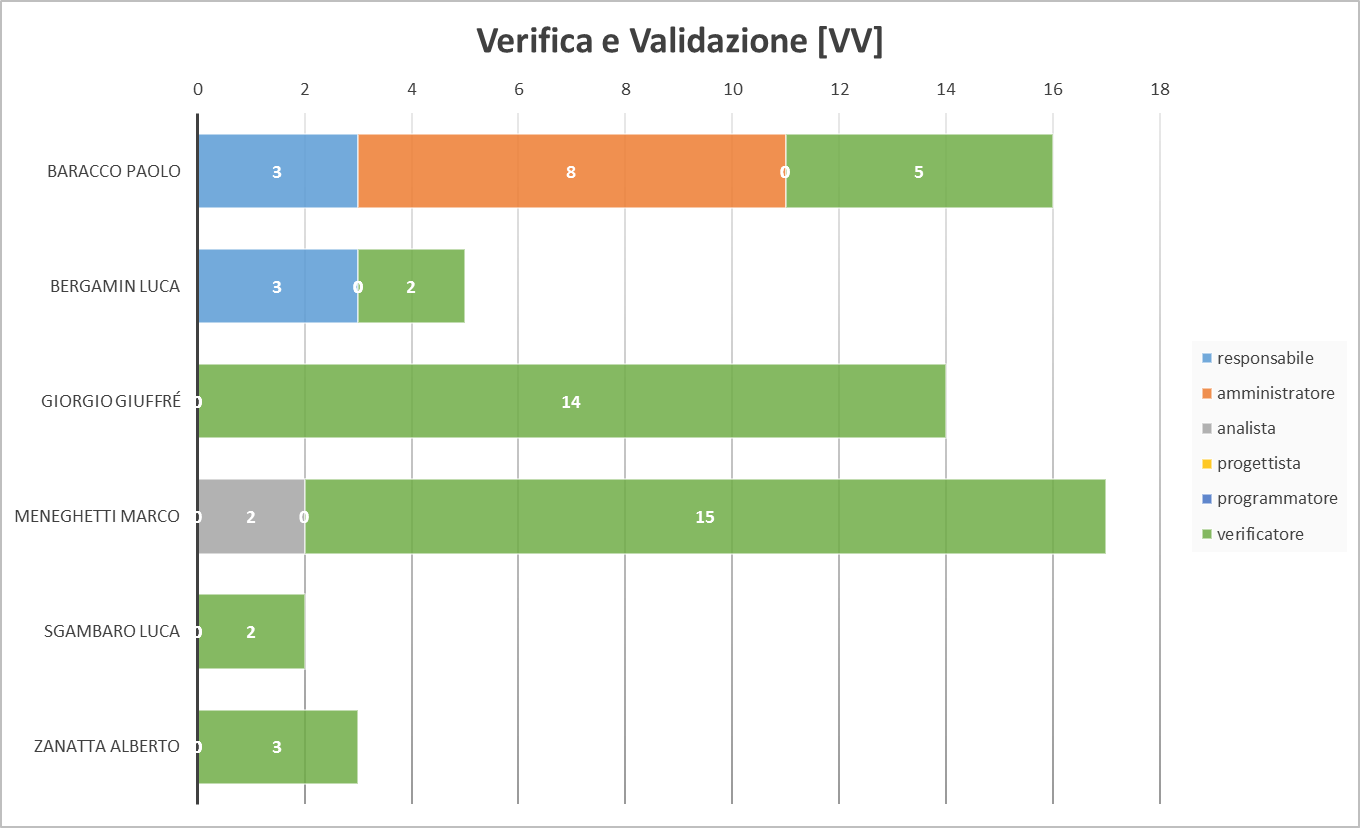
\includegraphics[width=1.1\textwidth]{img/orevv1.png}}
\caption{Ore/ruolo per persona durante la \VV.}
\label{fig:vv1}

\end{figure}

\begin{figure}[H]
\makebox[\textwidth][c]{
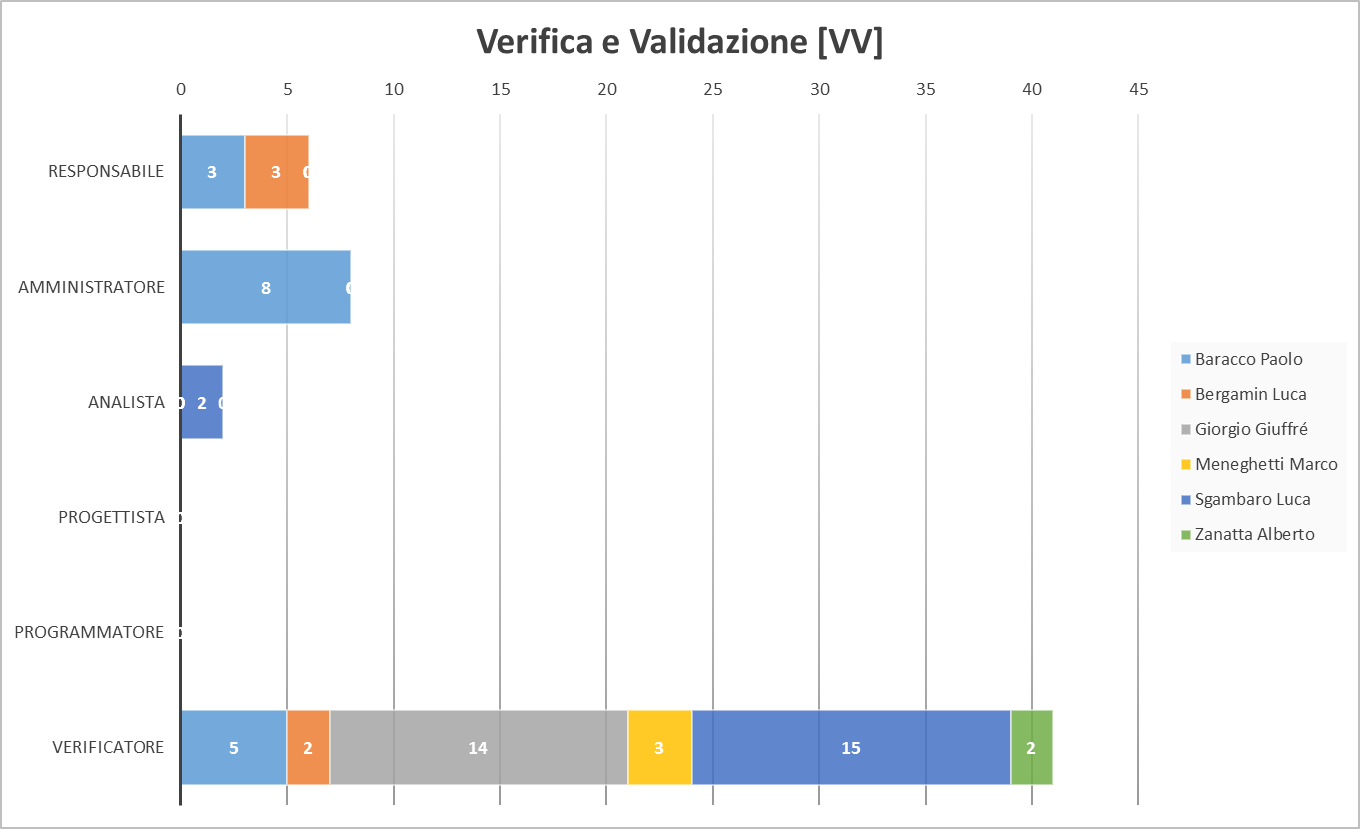
\includegraphics[width=1.1\textwidth]{img/orevv2.png}}
\caption{Ore/persona per ruolo durante la \VV.}
\label{fig:vv2}

\end{figure}


\pagebreak

\subsubsection{Costo \VV}
\introcosto{\VV}
Questa fase mira a completare tutte le attività di qualifica prefissate da {\hx}.

Gli sforzi maggiori si evidenziano nel ruolo di:
\begin{itemize}
\item {\Vx} per la verifica e validazione del prodotto creato.
\end{itemize}

\begin{figure}[H]
\makebox[\textwidth][c]
{
\definecolor{white2}{rgb}{0.95,0.95,0.95}
\definecolor{white3}{rgb}{0.9,0.9,0.9}
%\rowcolors{1}{white}{white2}

  \begin{tabular}{ | l | c | c | c | c | c | c | r |}
    \hline
    \rowcolor[gray]{.9}
    Ruolo / persona & \R & \AM & \AN & \PJ & \PG & \V & Tot euro/persona \\ \hline
    \PB & 90 & 160 & 0 & 0 & 0 & 75 & 325 \\ \hline
    \LB & 90 & 0 & 0 & 0 & 0 & 30 & 120 \\ \hline
    \GG & 0 & 0 & 0 & 0 & 0 & 210 & 210 \\ \hline
    \MM & 0 & 0 & 50 & 0 & 0 & 225 & 275 \\ \hline
    \LS & 0 & 0 & 0 & 0 & 0 & 30 & 30 \\ \hline
    \AZ & 0 & 0 & 0 & 0 & 0 & 45 & 45 \\ \hline
    \rowcolor[gray]{.9}

    Totale euro/ruolo & 180 & 160 & 50 & 0 & 0 & 615 & 1005 \\ \hline
  \end{tabular}
  
}\label{tab:vv}

  \caption{Tabella costo {\VV} per ruolo e per persona, valori in euro (\euro).}
\end{figure}

\begin{figure}[H]
\makebox[\textwidth][c]{
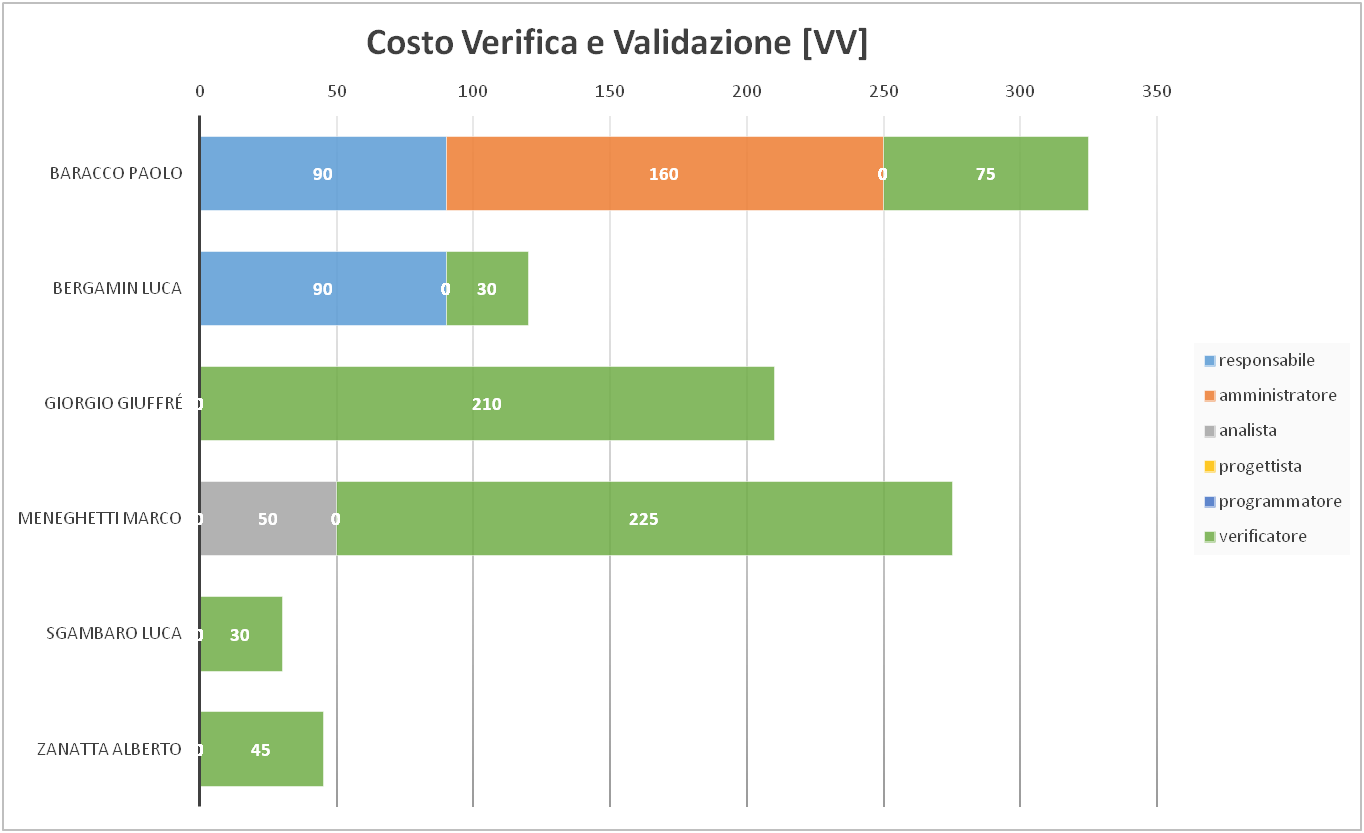
\includegraphics[width=1.2\textwidth]{img/costovv.png}}
\label{tab:cvv}

  \caption{Costo {\VV} per ruolo, valori in euro (\euro).}
\end{figure}

\pagebreak[4]

\subsection{Ore totali del progetto}
Di seguito si riporta la divisione oraria pianificata generale.

Successivamente sono evidenziate graficamente la divisione delle ore per persona e ruolo.

Questo quadro riassuntivo include il periodo di {\AR}, il quale \textbf{non è a carico del cliente}.

{\hx} complessivamente ritiene di aver diviso equamente il carico di lavoro. Ogni disparità a livello di periodo è bilanciata nei periodi successivi. 

Il quantitativo di ore preventivate totali è fissato a \textbf{809 ore}.

Si è raggiunto l'obiettivo prefissato di assegnare ogni ruolo a ciascun componente di {\hx} almeno una volta. Disparità in questo senso sono inevitabili: inevitabilmente è necessaria una o più "figure di riferimento" per ogni ruolo, che impieghino più risorse per raggiungere gli incarichi più gravosi.


\begin{figure}[H]
\definecolor{white2}{rgb}{0.95,0.95,0.95}
\definecolor{white3}{rgb}{0.9,0.9,0.9}
%\rowcolors{1}{white}{white2}

\makebox[\textwidth][c]
{
  \begin{tabular}[width=1.2\textwidth]{ | l | c | c | c | c | c | c | r |}
    \hline
    \rowcolor[gray]{.9}
    Ruolo / persona & \R & \AM & \AN & \PJ & \PG & \V & Tot ore/persona \\ \hline
    \PB & 10 & 11 & 14 & 44 & 30 & 25 & 134 \\ \hline
    \LB & 15 & 19 & 6 & 46 & 30 & 22 & 138 \\ \hline
    \GG & 3 & 29 & 8 & 45 & 30 & 23 & 138 \\ \hline
    \MM & 2 & 20 & 10 & 42 & 30 & 31 & 135 \\ \hline
    \LS & 2 & 5 & 17 & 46 & 30 & 34 & 134 \\ \hline
    \AZ & 3 & 9 & 21 & 41 & 30 & 29 & 133 \\ \hline
    \rowcolor[gray]{.9}

    Totale ore/ruolo & 35 & 93 & 76 & 264 & 180 & 164 & 809 \\ \hline
    
  \end{tabular}
  }
  
  \label{tab:gen}

  \caption{Tabella costo generale per ruolo e per persona, valori in euro (\euro).}
\end{figure} 
% i colori danno problemi di visualizzazione alle linee


È possibile ricavare interessanti statistiche dalla tabella (\ref{tab:gen}) e dal grafico di ripartizione oraria (\ref{fig:gen2}): % che riferimento ha inserito latex?
\begin{itemize}
\item Il ruolo {\Rx} richiede il quantitativo di ore minimo rispetto alle altre mansioni: inizialmente è richiesto uno sforzo maggiore per la stesura del \emph{Piano di Progetto}, ma superata la fase di {\AR} questo ruolo è richiesto in misura minore.
\item Il ruolo {\AMx} richiede una discreta quantità di ore soprattutto in fase di {\AR} per definire un ambiente di sviluppo ideale. Completata questa fase il ruolo è richiesto in misura minore.
\item Il ruolo {\ANx} richiede anch'esso la maggior parte delle ore in fase di {\AR} e successivamente sono ammessi solo incrementi del documento di {\AR}.
\item Il ruolo {\PJx} è ritenuto da {\hx} cruciale, dunque ne è stato assegnato il quantitativo maggiore di ore.
\item Il ruolo {\PGx} richiede una quantità di tempo pari a circa due terzi delle ore impiegate in fase di progettazione. Questa divisione a livello di preventivo è stata ritenuta accettabile, ma {\hx} si riserva di effettuare nuovamente questa analisi alla consegna del consuntivo finale.
\item Il ruolo {\Vx} richiede una quantità di tempo simile a quella riservata per il ruolo di {\PGx} e questa assegnazione è sembrata accettabile a livello di preventivo. {\hx} si riserva di effettuare nuovamente questa analisi alla consegna del consuntivo finale.
\end{itemize}



\pagebreak

\begin{figure}[H]
\makebox[\textwidth][c]{
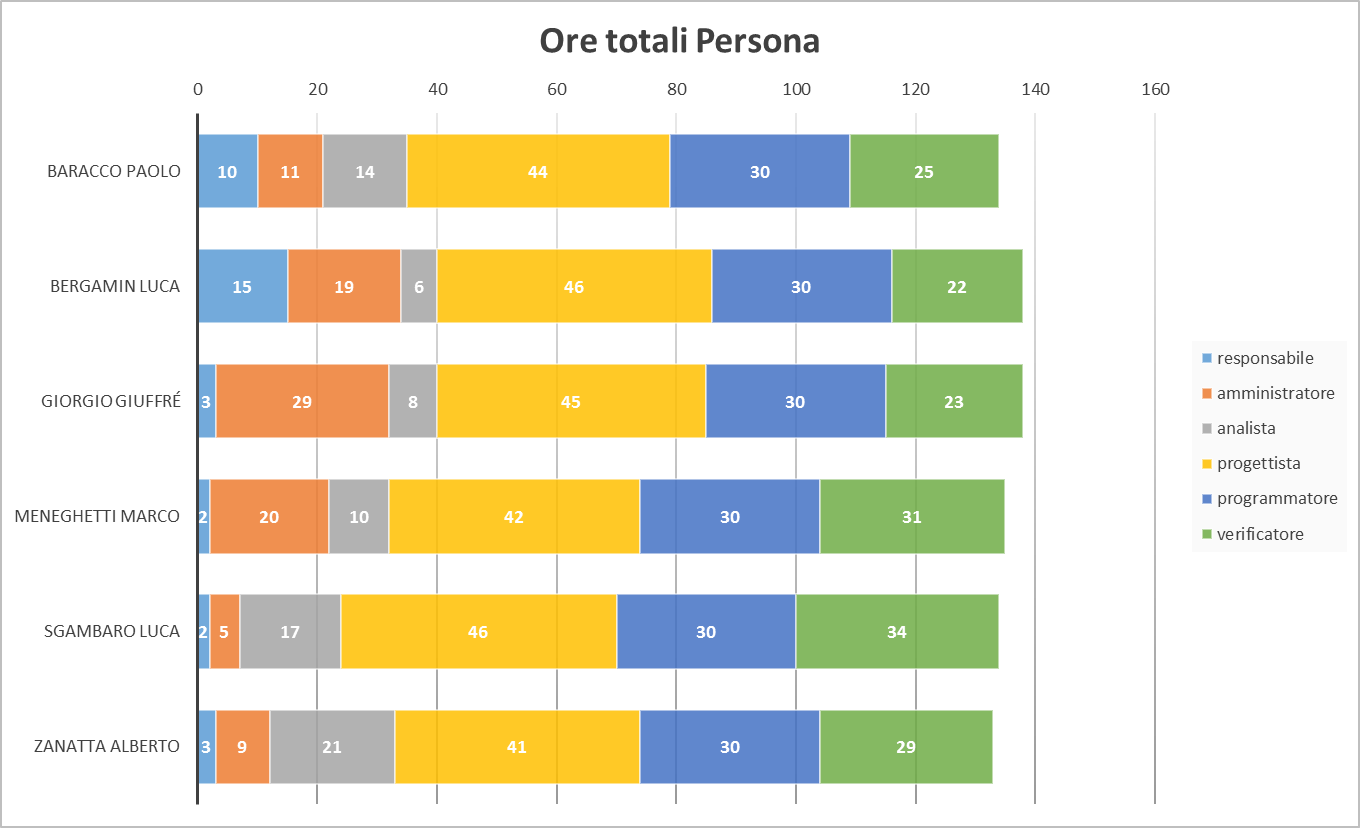
\includegraphics[width=1.1\textwidth]{img/oretotali1.png}}
\caption{Ore/ruolo per persona per il progetto \proj{}.}
\label{fig:gen1}

\end{figure}

\begin{figure}[H]
\makebox[\textwidth][c]{
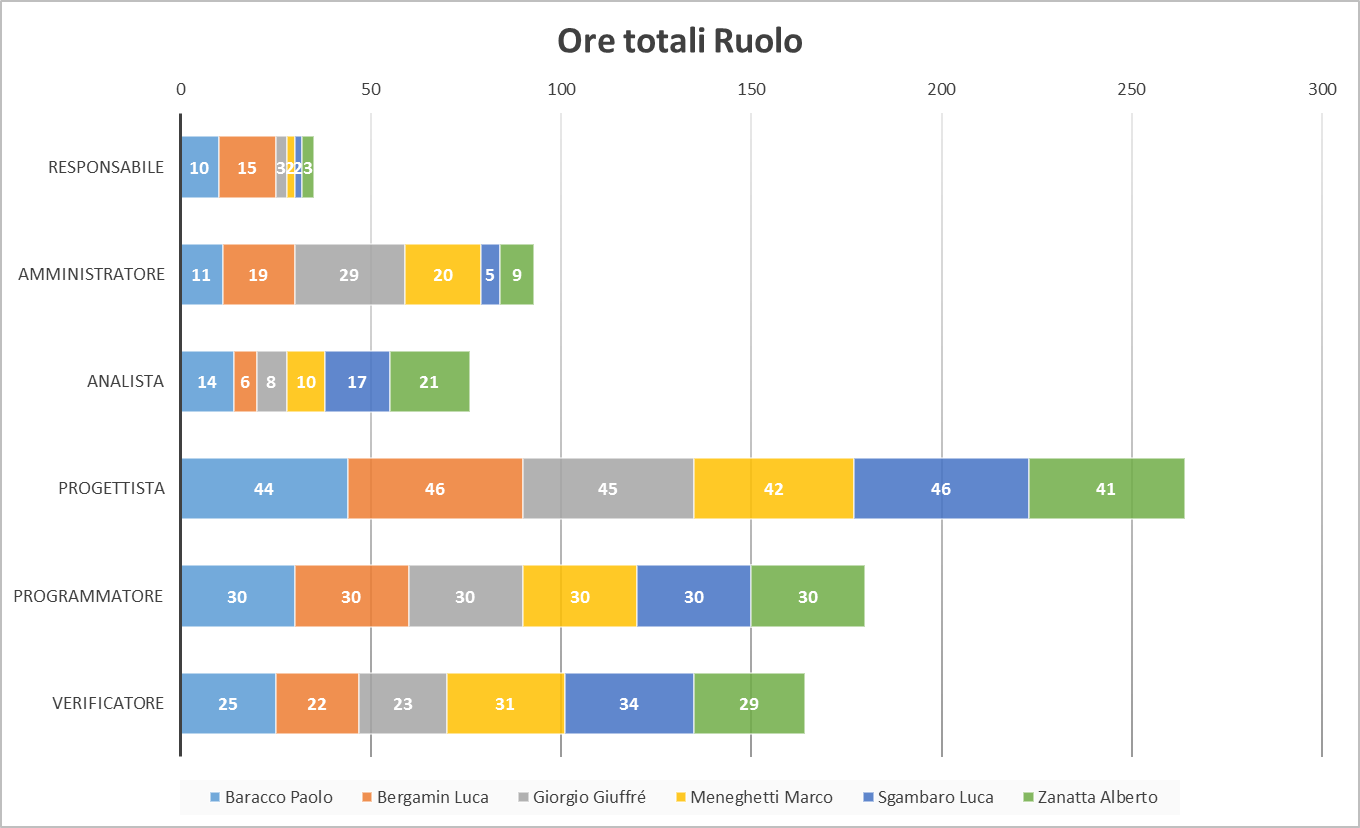
\includegraphics[width=1.1\textwidth]{img/oretotali2.png}}
\caption{Ore/persona per ruolo per il progetto \proj{}.}
\label{fig:gen2}

\end{figure}


\subsubsection{Costo ore totali del progetto}
Di seguito si riporta il costo delle ore totali, suddiviso per persona e ruolo.

Questo quadro riassuntivo include il periodo di {\AR}, il quale \textbf{non è a carico del cliente}.

\begin{figure}[H]
\makebox[\textwidth][c]
{
\definecolor{white2}{rgb}{0.95,0.95,0.95}
\definecolor{white3}{rgb}{0.9,0.9,0.9}
%\rowcolors{1}{white}{white2}

  \begin{tabular}{ | l | c | c | c | c | c | c | r |}
    \hline
    \rowcolor[gray]{.9}
    Ruolo / persona & \R & \AM & \AN & \PJ & \PG & \V & Tot euro/persona \\ \hline
    \PB & 300 & 220 & 350 & 968 & 450 & 375 & 2663 \\ \hline
    \LB & 450 & 380 & 150 & 1012 & 450 & 330 & 2772 \\ \hline
    \GG & 90 & 580 & 200 & 990 & 450 & 345 & 2655 \\ \hline
    \MM & 60 & 400 & 250 & 924 & 450 & 465 & 2549 \\ \hline
    \LS & 60 & 100 & 425 & 1012 & 450 & 510 & 2557 \\ \hline
    \AZ & 90 & 180 & 525 & 902 & 450 & 435 & 2582 \\ \hline
    \rowcolor[gray]{.9}

    Totale euro/ruolo & 1050 & 1860 & 1900 & 5808 & 2700 & 2460 & 15778 \\ \hline
  \end{tabular}
  
}\label{tab:cgen}

  \caption{Tabella costo totale per ruolo e per persona, valori in euro (\euro).}
\end{figure}

\begin{figure}[H]
\makebox[\textwidth][c]{
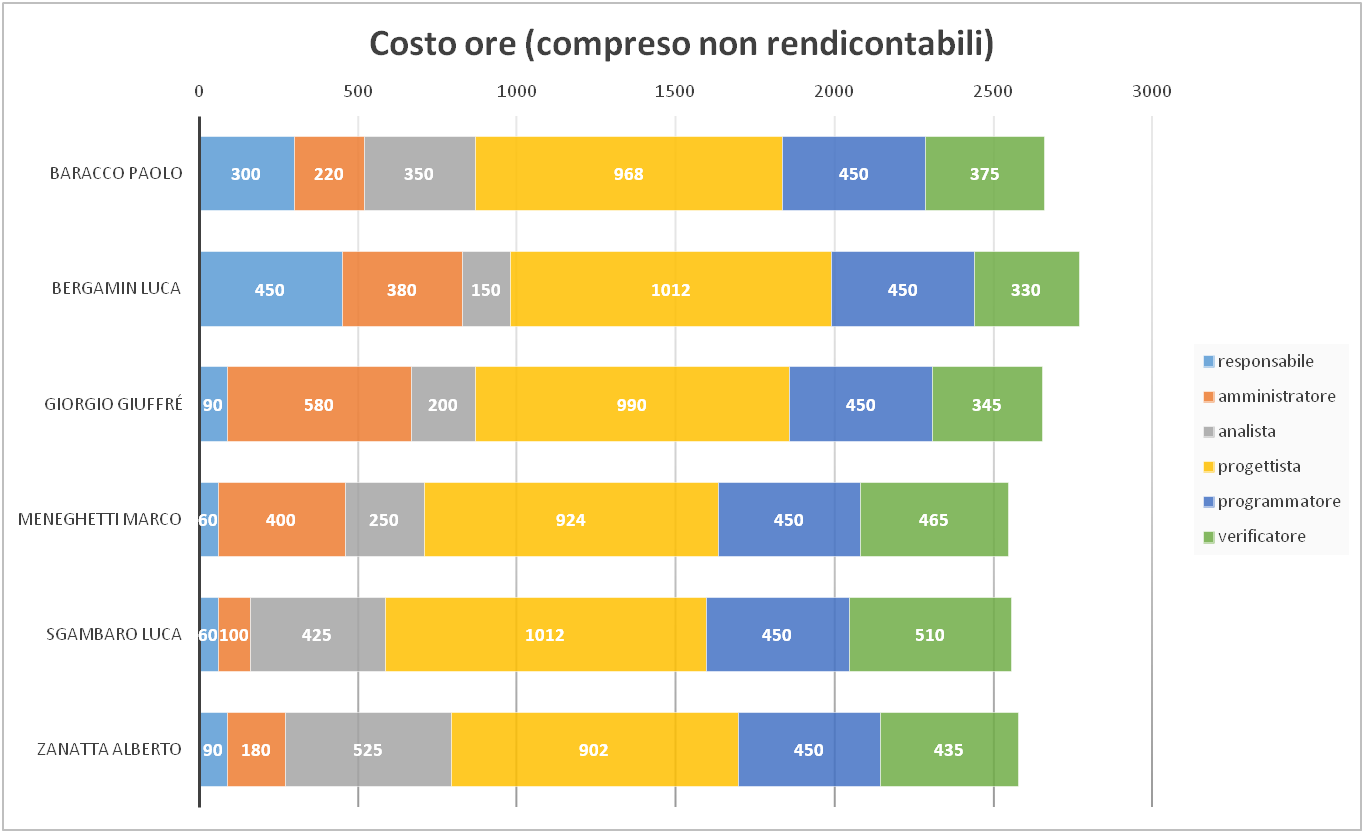
\includegraphics[width=1.2\textwidth]{img/costototale.png}}
\label{tab:cgen1}

  \caption{Costo totale per il progetto \proj{} per ruolo e per persona, valori in euro (\euro).}
\end{figure}


%si riporta pure oretotali4.png?
\pagebreak[4]



\subsection{Ore rendicontate del progetto} 
\label{sec:orerend}
%stessa cosa della sezione precedente
Di seguito si riporta la divisione oraria pianificata generale delle sole ore rendicontate.

Successivamente sono evidenziate graficamente la divisione delle ore per persona e ruolo.

Questo quadro riassuntivo esclude il periodo di {\AR}: il totale risultante \textbf{è a carico del cliente}.

Il quantitativo rendicontato a preventivo a persona è di \textbf{103 ore} e il quantitativo di ore preventivate totali è fissato a \textbf{618 ore}.

{\hx} complessivamente ritiene di aver diviso equamente il carico di lavoro, in quanto i scostamenti orari in misura minore del 5\%.

\begin{figure}[H]
\definecolor{white2}{rgb}{0.95,0.95,0.95}
\definecolor{white3}{rgb}{0.9,0.9,0.9}
%\rowcolors{1}{white}{white2}

\makebox[\textwidth][c]
{
  \begin{tabular}[width=1.2\textwidth]{ | l | c | c | c | c | c | c | r |}
    \hline
    \rowcolor[gray]{.9}
    Ruolo / persona & \R & \AM & \AN & \PJ & \PG & \V & Tot ore/persona \\ \hline
    \PB & 3 & 8 & 0 & 44 & 30 & 18 & 103 \\ \hline
    \LB & 3 & 8 & 0 & 46 & 30 & 16 & 103 \\ \hline
    \GG & 3 & 5 & 0 & 45 & 30 & 20 & 103 \\ \hline
    \MM & 2 & 0 & 2 & 42 & 30 & 27 & 103 \\ \hline
    \LS & 2 & 3 & 5 & 46 & 30 & 17 & 103 \\ \hline
    \AZ & 2 & 5 & 8 & 41 & 30 & 17 & 103 \\ \hline
    \rowcolor[gray]{.9}

    Totale ore/ruolo & 15 & 29 & 15 & 264 & 180 & 115 & 618 \\ \hline
    
  \end{tabular}
  }
  
  \label{tab:rend}

  \caption{Tabella costo generale per ruolo e per persona, valori in euro (\euro).}
\end{figure} 
% i colori danno problemi di visualizzazione alle linee


\subsubsection{Costo ore rendicontate del progetto}
Di seguito si riporta il costo delle ore totali rendicontate, suddiviso per persona e ruolo.

Questo quadro riassuntivo esclude il periodo di {\AR}: i costi che seguono \textbf{ sono a carico del cliente}.

\begin{figure}[H]
\makebox[\textwidth][c]
{
\definecolor{white2}{rgb}{0.95,0.95,0.95}
\definecolor{white3}{rgb}{0.9,0.9,0.9}
%\rowcolors{1}{white}{white2}

  \begin{tabular}{ | l | c | c | c | c | c | c | r |}
    \hline
    \rowcolor[gray]{.9}
    Ruolo / persona & \R & \AM & \AN & \PJ & \PG & \V & Tot euro/persona \\ \hline
    \PB & 90 & 160 & 0 & 968 & 450 & 270 & 1938 \\ \hline
    \LB & 90 & 160 & 0 & 1012 & 450 & 240 & 1952 \\ \hline
    \GG & 90 & 100 & 0 & 990 & 450 & 300 & 1930 \\ \hline
    \MM & 60 & 0 & 50 & 924 & 450 & 405 & 1889 \\ \hline
    \LS & 60 & 60 & 125 & 1012 & 450 & 255 & 1962 \\ \hline
    \AZ & 60 & 100 & 200 & 902 & 450 & 255 & 1967 \\ \hline
    \rowcolor[gray]{.9}

    Totale euro/ruolo & 450 & 580 & 375 & 5808 & 2700 & 1725 & 11638 \\ \hline
  \end{tabular}
  
}\label{tab:cgen}

  \caption{Tabella costo totale per ruolo e per persona, valori in euro (\euro).}
\end{figure}

Il costo totale del progetto \proj{} preventivato è arrotondato a \textbf{11700{\euro}} (\emph{undicimilaesettecento euro}).

\begin{figure}[H]
\makebox[\textwidth][c]{
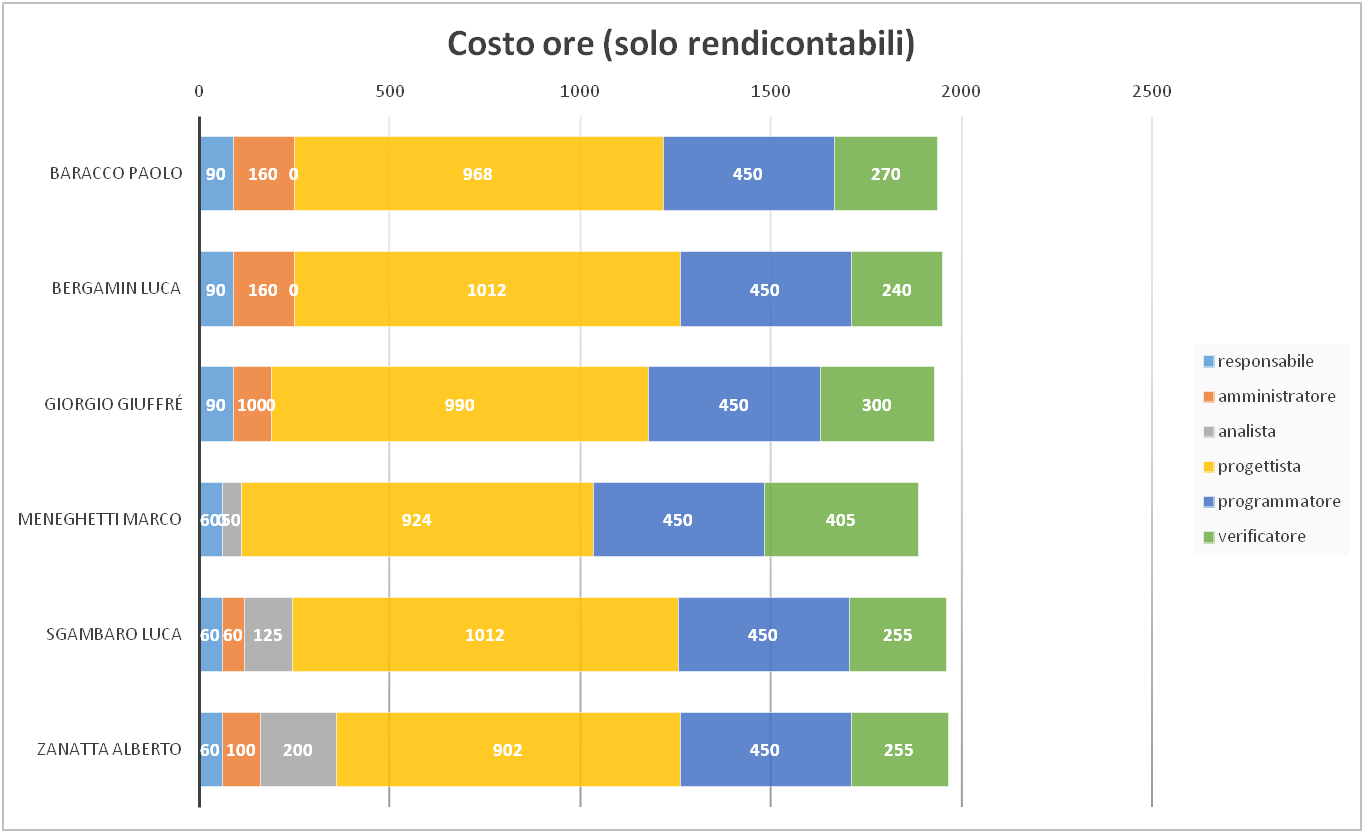
\includegraphics[width=1.2\textwidth]{img/costototalerendicontato.png}}
\label{tab:cgen1}

  \caption{Costo totale per il progetto \proj{} per ruolo e per persona, valori in euro (\euro).}
\end{figure}




\subsection{Ore non rendicontabili successive all'aggiudicazione dell'appalto}
Di seguito si riporta la divisione oraria pianificata generale delle ore non rendicontate a partire dalla \ARI, ovvero dalla aggiudicazione dell'appalto. Essa viene confrontata con il totale di ore rendicontate del progetto.
Il totale risultante ammonta a \textbf{923 ore}, pari al 60\% delle ore totali impiegate dal team per lo svolgimento del progetto. Si ricorda che tale sforzo \textbf{non è a carico del cliente}. Viene fornito a scopo informativo.

\begin{figure}[H]
\definecolor{white2}{rgb}{0.95,0.95,0.95}
\definecolor{white3}{rgb}{0.9,0.9,0.9}
%\rowcolors{1}{white}{white2}

\makebox[\textwidth][c]
{
  \begin{tabular}[width=1.2\textwidth]{ | l | c | c | c | c | c | c | r |}
    \hline
    \rowcolor[gray]{.9}
    Ruolo / persona & \R & \AM & \AN & \PJ & \PG & \V & Tot ore/persona \\ \hline
    \PB & 3/4 & 8/12 & 0 & 44/66 & 30/45 & 18/27 & 103/154 \\ \hline
    \LB & 3/6 & 8/12 & 0 & 46/69 & 30/45 & 16/24 & 103/156 \\ \hline
    \GG & 3/4 & 5/12 & 0 & 45/67 & 30/45 & 20/30 & 103/158 \\ \hline
    \MM & 2/4 & 0/10 & 2 & 42/63 & 30/45 & 27/40 & 103/162 \\ \hline
    \LS & 2/4 & 3/4 & 5 & 46/69 & 30/45 & 17/26 & 103/148 \\ \hline
    \AZ & 2/4 & 5/8 & 8 & 41/62 & 30/45 & 17/26 & 103/145 \\ \hline
    \rowcolor[gray]{.9}

    Totale ore/ruolo & 15/26 & 29/48 & 15/0 & 264/396 & 180/270 & 125/173 & 618/923 \\ \hline
    
  \end{tabular}
  }
  
  \label{tab:rend}

  \caption{Tabella ore rendicontate/ore non rendicontate da \ARI, per ruolo e per persona.}
\end{figure}

%%%%%%%%%%%%%%%%%%%%%%%%%
%%  Consuntivo di periodo
%%%%%%%%%%%%%%%%%%%%%%%%%

\section{Consuntivo di periodo} \label{sec:consuntivo}
In questa sezione sono indicate le spese affrontate a termine di ogni milestone interna. Queste andranno a sommarsi per infine stilare il consuntivo finale.



\newcommand{\introconsuntivo}[1]
{
Di seguito si riporta la divisione oraria effettivamente adottata nella fase di #1.

Successivamente sono evidenziate graficamente la divisione delle ore per persona e per ruolo. 

È inoltre riportata la variazione riportata rispetto alla \gloss{baseline} inizialmente stilata e infine l'eventuale variazione di costo rispetto al preventivo.
}

\subsection{Consuntivo \AR}
\introconsuntivo{\AR}

Si ricorda che questo costo viene fornito a scopo informativo e rappresenta l'investimento effettuato da {\hx} prima dell'aggiudicazione dell'appalto e perciò tale periodo \textbf{non è a carico del cliente}. 

\subsubsection{Variazioni nella pianificazione}

Qualora parte dei diagrammi non vengano riportati, si intende che essi hanno rispettato la corretta pianificazione, terminando in modo identico alla pianificazione.

\begin{figure}[H]
\makebox[\textwidth][c]{
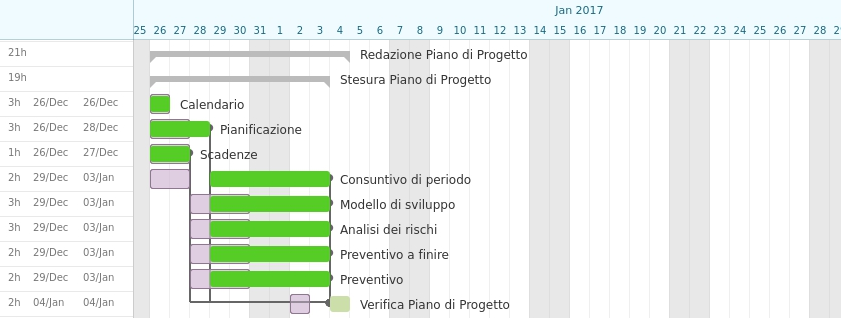
\includegraphics[width=1.2\textwidth]{img/ganttarc21.png}}
\label{tab:cgen1}

  \caption{Variazione rispetto alla pianificazione per l'\AR, diagramma di Gantt}
\end{figure}

Si è verificato un ritardo nella stesura del presente documento a causa di una influenza di un membro del gruppo in data 30-12-2016.

Questo ha portato un ritardo complessivo pari a 3 giorni rispetto alla baseline; tuttavia il task non ha portato ritardi se non all'attività di verifica relativa al documento stesso. L'attività \emph{Resoconto dell'attività di verifica} non ha subito ritardi a causa del grande gap temporale tra le due attività.

\pagebreak
\subsubsection{Variazione nei costi}
\begin{itemize}

\item Non sono state rilevate variazioni nei costi.

\item Non si riportano i grafici di variazione oraria.

\item Si riportano le tabelle di divisione oraria effettive e i relativi costi.

\end{itemize}
% i colori danno problemi di visualizzazione alle linee
\begin{figure}[H]
\makebox[\textwidth][c]
{
\definecolor{white2}{rgb}{0.95,0.95,0.95}
\definecolor{white3}{rgb}{0.9,0.9,0.9}
%\rowcolors{1}{white}{white2}

  \begin{tabular}{ | l | c | c | c | c | c | c | r |}
    \hline
    \rowcolor[gray]{.9}
    Ruolo / persona & \R & \AM & \AN & \PJ & \PG & \V & Tot ore/persona \\ \hline
    \PB & 7 & 3 & 14 & 0 & 0 & 7 & 31 \\ \hline
    \LB & 12 & 11 & 6 & 0 & 0 & 6 & 35 \\ \hline
    \GG & 0 & 24 & 8 & 0 & 0 & 3 & 35 \\ \hline
    \MM & 0 & 20 & 8 & 0 & 0 & 4 & 32\\ \hline
    \LS & 0 & 2 & 12 & 0 & 0 & 17 & 31\\ \hline
    \AZ & 1 & 4 & 13 & 0 & 0 & 12 & 30 \\ \hline
    \rowcolor[gray]{.9}

    Totale ore/ruolo & 20 & 64 & 61 & 0 & 0 & 49 & 194 \\ \hline
    
  \end{tabular}
}
\label{tab:car}
\caption{Tabella ore effettive {\AR} per ruolo e per persona.}

\end{figure}


\begin{figure}[H]
\makebox[\textwidth][c]
{
\definecolor{white2}{rgb}{0.95,0.95,0.95}
\definecolor{white3}{rgb}{0.9,0.9,0.9}
%\rowcolors{1}{white}{white2}

  \begin{tabular}{ | l | c | c | c | c | c | c | r |}
    \hline
    \rowcolor[gray]{.9}
    Ruolo / persona & \R & \AM & \AN & \PJ & \PG & \V & Tot euro/persona \\ \hline
    \PB & 210 & 60 & 350 & 0 & 0 & 105 & 725 \\ \hline
    \LB & 360 & 220 & 150 & 0 & 0 & 90 & 820 \\ \hline
    \GG & 0 & 480 & 200 & 0 & 0 & 45 & 725 \\ \hline
    \MM & 0 & 400 & 200 & 0 & 0 & 60 & 660 \\ \hline
    \LS & 0 & 40 & 300 & 0 & 0 & 255 & 595 \\ \hline
    \AZ & 30 & 80 & 325 & 0 & 0 & 180 & 615 \\ \hline
    \rowcolor[gray]{.9}

    Totale euro/ruolo & 600 & 1280 & 1525 & 0 & 0 & 735 & 4140 \\ \hline
  \end{tabular}
  
}
\label{tab:car}
\caption{Tabella costo effettivo {\AR} per ruolo e per persona, valori in euro (\euro).}
\end{figure}

\begin{figure}[H]
\makebox[\textwidth][c]
{
\definecolor{white2}{rgb}{0.95,0.95,0.95}
\definecolor{white3}{rgb}{0.9,0.9,0.9}
%\rowcolors{1}{white}{white2}

  \begin{tabular}{ | l | c | r |}
    \hline
    \rowcolor[gray]{.9}
    Ruolo  & Ore & Costo \\ \hline
    \R & 20 & 600 \\ \hline
    \AM & 64 & 1280 \\ \hline
    \AN & 61 & 1525 \\ \hline
    \V & 49 & 735 \\ \hline
    \rowcolor[gray]{.9}

   Differenza & 0 & 0 \\ \hline
  \end{tabular}
  
}
\label{tab:car}
\caption{Differenza preventivo-consuntivo per ruolo, \AR.}
\end{figure}


\subsubsection{Considerazioni}
La pianificazione è stata in gran parte rispettata, eccetto un trascurabile ritardo per malattia. 

Un aspetto trascurato potenzialmente migliorativo della pianificazione corrente consiste nell'includere nella pianificazione delle attività anche degli incontri con l'azienda \ZU, accordandosi preventivamente, in modo da poter avere dei rapporti continui con l'azienda proponente. Questa opzione sarà considerata dal \Rx{} nei periodi successivi.

%%%%%%%% da fare%%%%%%%%%%%%%%%%%%%%%%%%%%%%%%%%%%%%%%%%%%%%%%%%%%%%%%%%%%%%%%%%%%


\pagebreak
\subsection{Consuntivo \ARI}
\introconsuntivo{\ARI}

\subsubsection{Variazioni nella pianificazione}

\begin{figure}[H]
\makebox[\textwidth][c]{
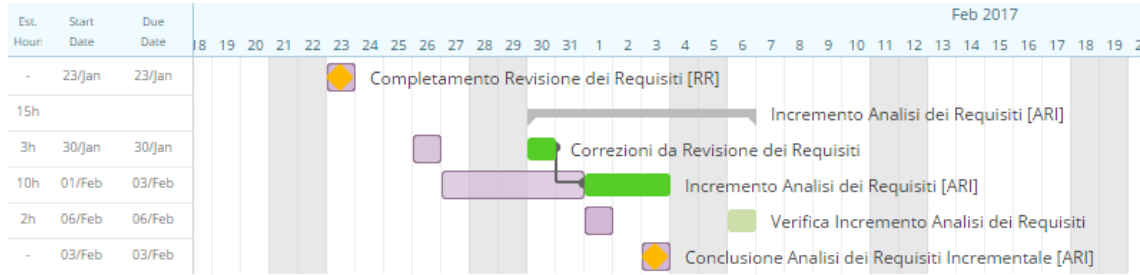
\includegraphics[width=1.2\textwidth]{img/varari.png}}
\label{tab:cgen1}

  \caption{Variazione rispetto alla pianificazione per l'\ARI, diagramma di Gantt}
\end{figure}

Si è verificato un ritardo nell'attuazione dei task previsti per la \ARI{} a causa della necessità di alcuni membri del gruppo di sostenere altri esami relativi al Corso di Laurea in Informatica. Questo ha portato ad un ritardo delle attività le quali sono cominciate il giorno 30-01-2017, ovvero con 4 giorni di ritardo.

Questo ritardo comunque non ha influenzato eccessivamente gli altri task, i quali sono stati effettuati senza ritardi accumulati, svolgendo dapprima lavoro non relativo all'incremento effettuato.


\pagebreak
\subsubsection{Variazione nei costi}
\begin{itemize}

\item Non sono state rilevate variazioni nei costi.

\item Non si riportano i grafici di variazione oraria.

\item Si riportano le tabelle di divisione oraria effettive e i relativi costi.

\end{itemize}
% i colori danno problemi di visualizzazione alle linee
\begin{figure}[H]
\makebox[\textwidth][c]
{
\definecolor{white2}{rgb}{0.95,0.95,0.95}
\definecolor{white3}{rgb}{0.9,0.9,0.9}
%\rowcolors{1}{white}{white2}

  \begin{tabular}{ | l | c | c | c | c | c | c | r |}
    \hline
    \rowcolor[gray]{.9}
    Ruolo / persona & \R & \AM & \AN & \PJ & \PG & \V & Tot ore/persona \\ \hline
    \PB & 0 & 0 & 0 & 0 & 0 & 0 & 0 \\ \hline
    \LB & 0 & 0 & 0 & 0 & 0 & 0 & 0 \\ \hline
    \GG & 0 & 0 & 0 & 0 & 0 & 2 & 2 \\ \hline
    \MM & 0 & 0 & 0 & 0 & 0 & 0 & 0 \\ \hline
    \LS & 0 & 0 & 5 & 0 & 0 & 0 & 5 \\ \hline
    \AZ & 0 & 0 & 8 & 0 & 0 & 0 & 8 \\ \hline
    \rowcolor[gray]{.9}

    Totale ore/ruolo & 0 & 0 & 13 & 0 & 0 & 2 & 15 \\ \hline
    
  \end{tabular}
}
\label{tab:car}
\caption{Tabella ore effettive {\ARI} per ruolo e per persona.}

\end{figure}


\begin{figure}[H]
\makebox[\textwidth][c]
{
\definecolor{white2}{rgb}{0.95,0.95,0.95}
\definecolor{white3}{rgb}{0.9,0.9,0.9}
%\rowcolors{1}{white}{white2}

  \begin{tabular}{ | l | c | c | c | c | c | c | r |}
    \hline
    \rowcolor[gray]{.9}
    Ruolo / persona & \R & \AM & \AN & \PJ & \PG & \V & Tot euro/persona \\ \hline
    \PB & 0 & 0 & 0 & 0 & 0 & 0 & 0 \\ \hline
    \LB & 0 & 0 & 0 & 0 & 0 & 0 & 0 \\ \hline
    \GG & 0 & 0 & 0 & 0 & 0 & 30 & 30 \\ \hline
    \MM & 0 & 0 & 0 & 0 & 0 & 0 & 0 \\ \hline
    \LS & 0 & 0 & 125 & 0 & 0 & 0 & 125 \\ \hline
    \AZ & 0 & 0 & 200 & 0 & 0 & 0 & 200 \\ \hline
    \rowcolor[gray]{.9}

    Totale euro/ruolo & 0 & 0 & 325 & 0 & 0 & 30 & 355 \\ \hline
  \end{tabular}
  
}\label{tab:cari}

  \caption{Tabella costo {\ARI} per ruolo e per persona, valori in euro (\euro).}
\end{figure}

\begin{figure}[H]
\makebox[\textwidth][c]
{
\definecolor{white2}{rgb}{0.95,0.95,0.95}
\definecolor{white3}{rgb}{0.9,0.9,0.9}
%\rowcolors{1}{white}{white2}

  \begin{tabular}{ | l | c | r |}
    \hline
    \rowcolor[gray]{.9}
    Ruolo  & Ore & Costo \\ \hline
    \AN & 13 & 325 \\ \hline
    \V & 2 & 30 \\ \hline
    \rowcolor[gray]{.9}

   Differenza & 0 & 0 \\ \hline
  \end{tabular}
  
}
\label{tab:car}
\caption{Differenza preventivo-consuntivo per ruolo, \ARI.}
\end{figure}



\subsubsection{Considerazioni}
La pianificazione è stata rispettata ad un livello sub-ottimale, ma comunque accettabile. Il \Rx{} terrà in maggior conto gli impegni universitari dei componenti del gruppo, prevedendo anche la necessità di ritentare più volte un esame.

L'utilità di questo periodo è stata inferiore a quanto preventivato: la sua ridotta dimensione è risultata troppo dispersiva.

%%%%%%%%%%%%%%%%%%%%%%%%%%%%%%%%%%%%%%%%%%%%%%%%%%%%%%%%%%%%%%%%%%%%%%%%%%%%%%%%%%%%%%%%%%%%%%%%%
\subsection{Consuntivo \PA}
\introconsuntivo{\PA}

\subsubsection{Variazioni nella pianificazione}

Qualora parte dei diagrammi non vengano riportati, si intende che essi hanno rispettato la corretta pianificazione, terminando in modo identico alla pianificazione.

\begin{figure}[H]
\makebox[\textwidth][c]{
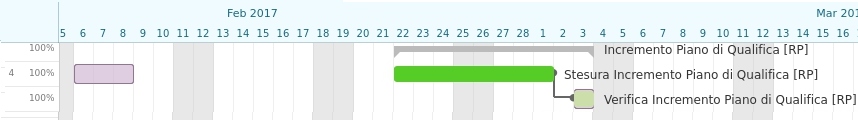
\includegraphics[width=1.2\textwidth]{img/varpa3.png}}
\label{tab:cgen1}

\caption{Variazione rispetto alla pianificazione per la \PA{} diagramma di Gantt (parte 1)}
\end{figure}

Si è verificato un ritardo nella stesura dei documenti del \PdQ{} a causa del carico di lavoro sottostimato a preventivo per la correzione degli errori risultante dalla prima revisione di avanzamento. All'attività \emph{Stesura Incremento Piano di Qualifica [RP]} è stata dunque riservata un periodo temporale più lungo e maggiori risorse, sottraendole dall'attività di progettazione. La data d'inizio di tale attività, a causa della riunione organizzata dal \TV{} del 21-02-2017, è stata spostata dal giorno 6-02-2017 al giorno 22-02-2017. Ulteriori osservazioni sono descritte dopo la seguente sezione.


\begin{figure}[H]
\makebox[\textwidth][c]{
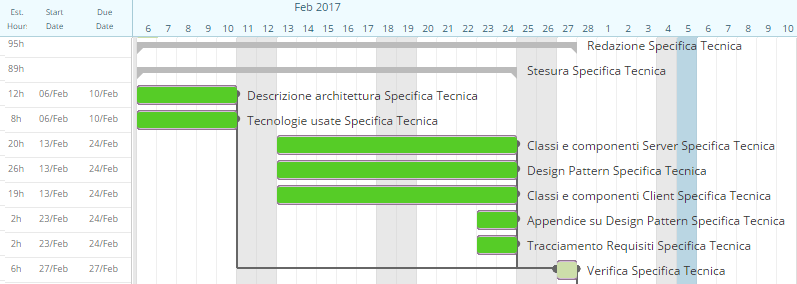
\includegraphics[width=1.2\textwidth]{img/varpa2.png}}
\label{tab:cgen1}

\caption{Variazione rispetto alla pianificazione per la \PA{} diagramma di Gantt (parte 2)}
\end{figure}

È stato cambiato il nome del task \emph{Diagrammi di attività Specifica Tecnica}, in quanto errata nella fase di \PA{} ed è stato variato il nome in \emph{Componenti e classi Client Specifica Tecnica} e \emph{Componenti e classi Server Specifica Tecnica}.

Le ore dedicate al task \emph{Redazione Specifica Tecnica} sono variate, da un totale di 114 ore a 95 ore, per una variazione negativa di 19 ore.

Le ore dedicate al task \emph{Incremento Piano di Qualifica [RP]} sono variate, da un totale di 5 ore a 28 ore, per una variazione positiva di 23 ore.



%Si è verificato un ritardo nella stesura del presente documento a causa di una influenza di un membro del gruppo in data 30-12-2016.

%Questo ha portato un ritardo complessivo pari a 3 giorni rispetto alla baseline; tuttavia il task non ha portato ritardi se non all'attività di verifica relativa al documento stesso. L'attività \emph{Resoconto dell'attività di verifica} non ha subito ritardi a causa del grande gap temporale tra le due attività.

\pagebreak
\subsubsection{Variazione nei costi}
\begin{itemize}

\item Sono state rilevate variazioni nei costi.

\item Si riportano le tabelle di divisione oraria effettive e i relativi costi.

\end{itemize}
% i colori danno problemi di visualizzazione alle linee
\begin{figure}[H]
\definecolor{white2}{rgb}{0.95,0.95,0.95}
\definecolor{white3}{rgb}{0.9,0.9,0.9}
%\rowcolors{1}{white}{white2}

\makebox[\textwidth][c]
{
  \begin{tabular}{ | l | c | c | c | c | c | c | r |}
    \hline
    \rowcolor[gray]{.9}
    Ruolo / persona & \R & \AM & \AN & \PJ & \PG & \V & Tot ore/persona \\ \hline
    \PB & 0 & 0 & 0 & 26 & 0 & 6 & 32 \\ \hline
    \LB & 0 & 3 & 0 & 38 & 0 & 1 & 42 \\ \hline
    \GG & 3 & 0 & 0 & 35 & 0 & 1 & 39 \\ \hline
    \MM & 0 & 0 & 0 & 39 (-3) & 0 & 7 (+3) & 46 \\ \hline
    \LS & 2 & 0 & 0 & 28 (-8) & 0 & 16 (+10) & 46 (+2) \\ \hline
    \AZ & 0 & 0 & 0 & 23 (-8) & 0 & 14 (+10) & 37 (+2) \\ \hline
    \rowcolor[gray]{.9}

    Totale ore/ruolo & 5 & 3 & 0 & 189 (-19) & 0 & 45 (+23) & 242 (+4) \\ \hline
    
  \end{tabular}
}
\caption{Ore/ruolo per persona durante la \PA.}
\end{figure} 


\begin{figure}[H]
\makebox[\textwidth][c]
{
\definecolor{white2}{rgb}{0.95,0.95,0.95}
\definecolor{white3}{rgb}{0.9,0.9,0.9}
%\rowcolors{1}{white}{white2}

  \begin{tabular}{ | l | c | c | c | c | c | c | r |}
    \hline
    \rowcolor[gray]{.9}
    Ruolo / persona & \R & \AM & \AN & \PJ & \PG & \V & Tot euro/persona \\ \hline
    \PB & 0 & 0 & 0 & 572 & 0 & 90 & 662 \\ \hline
    \LB & 0 & 60 & 0 & 836 & 0 & 15 & 911 \\ \hline
    \GG & 90 & 0 & 0 & 770 & 0 & 15 & 875 \\ \hline
    \MM & 0 & 0 & 0 & 858 (-66) & 0 & 105 (+45) & 963 (-21)\\ \hline
    \LS & 60 & 0 & 0 & 616 (-176) & 0 & 240 (+150) & 916 (-26)\\ \hline
    \AZ & 0 & 0 & 0 & 506 (-176) & 0 & 210 (+150) & 716 (-26)\\ \hline
    \rowcolor[gray]{.9}

    Totale euro/ruolo & 150 & 60 & 0 & 4158 (-418) & 0 & 675 (+345) & 5043 (-73)\\ \hline
    
  \end{tabular}
  
}\label{tab:cpa}

  \caption{Tabella costo {\PA} per ruolo e per persona, valori in euro (\euro).}
\end{figure}

\begin{figure}[H]
\makebox[\textwidth][c]
{
\definecolor{white2}{rgb}{0.95,0.95,0.95}
\definecolor{white3}{rgb}{0.9,0.9,0.9}
%\rowcolors{1}{white}{white2}

  \begin{tabular}{ | l | c | r |}
    \hline
    \rowcolor[gray]{.9}
    Ruolo  & Ore & Costo \\ \hline
    \R & 5 & 150 \\ \hline
    \AM & 3 & 60 \\ \hline
    \PJ & 189 (-19) & 4158 (-418)\\ \hline
    \V & 45 (+23) & 675 (+345) \\ \hline
    \rowcolor[gray]{.9}

   Differenza & +4 & -73 \\ \hline
  \end{tabular}
  
}
\label{tab:car}
\caption{Differenza preventivo-consuntivo per ruolo, \PA. Colonna \emph{Costo} in euro (\euro).}
\end{figure}

\subsubsection{Considerazioni}
A fronte delle necessarie correzioni al \PdQ{} non previste è stato necessario rivedere la pianificazione, sottraendo risorse alla progettazione e assegnandole alla verifica. Questo ha portato ad una variazione totale delle ore/persona del gruppo ma è sempre stato rispettato il vincolo delle 105 ore rendicontabili. 

\subsubsection{Preventivo a finire}
Il consuntivo presenta una differenza di costo negativa a causa del costo diverso delle due diverse mansioni. Queste risorse risparmiate in questa fase saranno investite successivamente qualora necessario al fine di migliorare ulteriormente le attività di verifica, prevedendo l'assegnazione di più ore alla attività di verifica. L'effettiva variazione delle ore assegnate sarà presentata nei prossimi consuntivi di periodo.

%%%%%%%%%%%%%%%%%%%%%%%%%%%%%%%%%%%%%%%%%%%%%%%%%%%%%%%%%%%%%%%%%%%%%%%%%%


%%%%%%%%%%%%%%%%%%%%%%%%%%%%%%%%%%%%%%%%%%%%%%%%%%%%%%%%%%%%%%%%%%%%%%%%%%%%%%%%%%%%%%%%%%%%%%%%%
\pagebreak
\subsection{Consuntivo \PDC}
\introconsuntivo{\PDC}

\subsubsection{Variazioni nella pianificazione}

Qualora parte dei diagrammi non vengano riportati, si intende che essi hanno rispettato la corretta pianificazione, terminando in modo identico alla pianificazione.

\begin{figure}[H]
\makebox[\textwidth][c]{
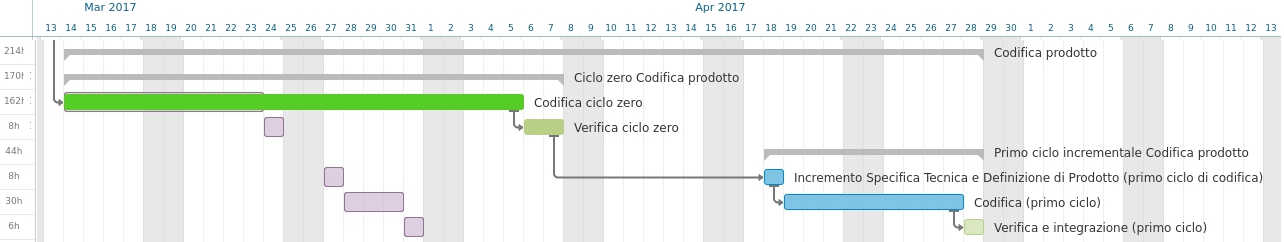
\includegraphics[width=1.2\textwidth]{img/varpdc1.png}}
\label{tab:cgen1}

\caption{Variazione rispetto alla pianificazione per la \PDC{} diagramma di Gantt (parte 1)}
\end{figure}

Si è verificato un grave rallentamento delle attività di verifica delle attività di codifica, la quale ha impedito sia il raggiungimento della creazione di un prodotto completo, sia l'attuazione del modello incrementale inizialmente proposto.

Tra le cause del rallentamento delle attività di codifica, passate da due a quattro settimane, si riscontra:
\begin{itemize}
\item stima troppo ottimistica del tempo necessario all'attività di codifica;
\item stima troppo ottimistica del tempo necessario all'attività di formazione sulle tecnologie utilizzate;
\item difficoltà nell'individuazione degli strumenti necessari ai test di unità.
\end{itemize}

Tale rallentamento ha portato ad uno slittamento delle attività di codifica pari a 3 settimane, prevedendo la terminazione del primo ciclo incrementale dal preventivato 07-04-2017 al 28-04-2017.

È stato deciso inoltre di eliminare il secondo ciclo incrementale, in quanto:
\begin{itemize}
\item poco adattabile alle esigenze delle revisioni di progetto: normalmente, collocare più di una attività di incremento all'interno di un unico periodo tra una revisione di progetto e l'altra risulta inutilmente dispersivo;
\item difficile da conciliare con le risorse rimanenti a disposizione.
\end{itemize}

Il gap di una settimana pianificato dal 10-04-2017 al 17-04-2017 è stato previsto per permettere al team di svolgere altre attività di carattere accademico non inerenti al progetto.

\begin{figure}[H]
\makebox[\textwidth][c]{
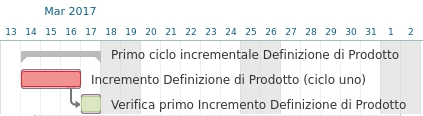
\includegraphics[width=0.5\textwidth]{img/varpdc2.png}}
\label{tab:cgen1}

\caption{Variazione rispetto alla pianificazione per la \PDC{} diagramma di Gantt (parte 2)}
\end{figure}

Sono state ridotte le attività e le ore previste per la stesura della Definizione di Prodotto, in quanto presentata solo a carattere informativo e non valutabile dal \TV. Ciò ha permesso di:

\begin{itemize}
\item Ridistribuire le ore alle attività che ne necessitavano (future attività di codifica e verifica);
\item Riassegnare il carico di lavoro rendicontabile bilanciandolo più nella \VV: questo non perché il team abbia lavorato in meno rispetto alle aspettative, ma perché le attività non rendicontabili hanno preso più tempo di quanto preventivato.
\end{itemize}

Si segnala quindi che le ore variate come indicato nella prossima sezione non rappresentano un risparmio, ma la riassegnazione delle attività. Si consulti il preventivo a finire relativo per ulteriori dettagli sulla nuova pianificazione.  

\pagebreak
\subsubsection{Variazione nei costi}
\begin{itemize}

\item Sono state rilevate variazioni nei costi.

\item Si riportano le tabelle di divisione oraria effettive e i relativi costi.

\end{itemize}

\begin{figure}[H]
\definecolor{white2}{rgb}{0.95,0.95,0.95}
\definecolor{white3}{rgb}{0.9,0.9,0.9}
%\rowcolors{1}{white}{white2}

\makebox[\textwidth][c]
{
  \begin{tabular}{ | l | c | c | c | c | c | c | r |}
    \hline
    \rowcolor[gray]{.9}
    Ruolo / persona & \R & \AM & \AN & \PJ & \PG & \V & Tot ore/persona \\ \hline
    \PB & 0 & 0 & 0 & 0 (-18) & 27 (-3) & 7 & 34 (-21) \\ \hline
    \LB & 0 & 5 & 0 & 0 (-8) & 27 (-3) & 11 (-2) & 43 (-13) \\ \hline
    \GG & 0 & 5 & 0 & 0 (-10) & 27 (-3) & 3 & 35 (-13) \\ \hline
    \MM & 2 & 0 & 0 & 0 & 27 (-3) & 4 (-4) & 33 (-7) \\ \hline
    \LS & 0 & 3 & 0 & 0 (-10) & 27 (-3) & 3 (-6) & 33 (-19) \\ \hline
    \AZ & 2 & 5 & 0 & 0 (-10) & 27 (-3) & 4 (-6) & 38 (-19) \\ \hline
    \rowcolor[gray]{.9}

    Totale ore/ruolo & 4 & 18 & 0 & 0 (-56) & 162 (-18) & 32 (-18) & 216 (-92) \\ \hline
    
  \end{tabular}
  }
    \caption{Ore/ruolo per persona durante la \PDC.}

\end{figure} 
% i colori danno problemi di visualizzazione alle linee

\begin{figure}[H]
\makebox[\textwidth][c]
{
\definecolor{white2}{rgb}{0.95,0.95,0.95}
\definecolor{white3}{rgb}{0.9,0.9,0.9}
%\rowcolors{1}{white}{white2}

  \begin{tabular}{ | l | c | c | c | c | c | c | r |}
    \hline
    \rowcolor[gray]{.9}
    Ruolo / persona & \R & \AM & \AN & \PJ & \PG & \V & Tot euro/persona \\ \hline
    \PB & 0 & 0 & 0 & 0 (-396) & 450 (-45) & 105 & 510 (-441) \\ \hline
    \LB & 0 & 100 & 0 & 0 (-176) & 450 (-45) & 165 (-30) & 670 (-251) \\ \hline
    \GG & 0 & 100 & 0 & 0 (-220) & 450 (-45) & 45 & 550 (-301) \\ \hline
    \MM & 60 & 0 & 0 & 0 & 450 (-45) & 60 (-60) & 525 (-105) \\ \hline
    \LS & 0 & 60 & 0 & 220 & 0 (-450) & 45 (-90) & 510 (-355) \\ \hline
    \AZ & 60 & 100 & 0 & 220 & 0 (-450) & 60 (-90) & 625 (-355) \\ \hline
    \rowcolor[gray]{.9}

    Totale euro/ruolo & 120 & 360 & 0 & 0 (-1232) & 2430 (-270) & 480 (-270) & 3390 (-1772) \\ \hline
  \end{tabular}
  
}\label{tab:cpdc}

  \caption{Tabella costo {\PDC} per ruolo e per persona, valori in euro (\euro).}
\end{figure}


%%%% DA FARE ANCORA (so' stanco)
\begin{figure}[H]
\makebox[\textwidth][c]
{
\definecolor{white2}{rgb}{0.95,0.95,0.95}
\definecolor{white3}{rgb}{0.9,0.9,0.9}
%\rowcolors{1}{white}{white2}

  \begin{tabular}{ | l | c | r |}
    \hline
    \rowcolor[gray]{.9}
    Ruolo  & Ore & Costo \\ \hline
    \R & 4 & 120 \\ \hline
    \AM & 18 & 360 \\ \hline
    \PJ & 0 (-56) & 0 (-1232)\\ \hline
    \PG & 162 (-18) & 2430 (-270) \\ \hline
    \V & 32 (-18) & 480 (-270) \\ \hline
    \rowcolor[gray]{.9}

   Differenza & -92 & -1772 \\ \hline
  \end{tabular}
  
}

\label{tab:car}
\caption{Differenza preventivo-consuntivo per ruolo, \PDC. Colonna \emph{Costo} in euro (\euro).}
\end{figure}

\subsubsection{Considerazioni}
A fronte della scelta presa di riequilibrare il carico, si presenta successivamente il nuovo preventivo a finire.

Si segnala che la cifra risparmiata nel periodo di \PA{}, pari a 73\euro{}, è stata reinvestita nella \VV a supporto di attività di verifica e test.

Non sono state portate a termine tutte le attività di codifica dei test, in particolare i test di sistema ed integrazione: tuttavia essi sono stati specificati all'interno del documento \emph{Piano di Qualifica}.

%Il \Rx{} ha tentato di incentivare il gruppo ad utilizzare Github Issues al fine tracciare 

\subsubsection{Nuova pianificazione}
Si riporta la nuova pianificazione del periodo \VV{}.

\begin{figure}[H]
\definecolor{white2}{rgb}{0.95,0.95,0.95}
\definecolor{white3}{rgb}{0.9,0.9,0.9}
%\rowcolors{1}{white}{white2}

\makebox[\textwidth][c]
{
  \begin{tabular}[width=1.2\textwidth]{ | l | c | c | c | c | c | c | r |}
    \hline
    \rowcolor[gray]{.9}
    Ruolo / persona & \R & \AM & \AN & \PJ & \PG & \V & Tot ore/persona \\ \hline
    \PB & 3 & 8 & 0 & 8 (+8) & 0 & 19 (+14) & 38 (+22) \\ \hline
    \LB & 3 & 0 & 0 & 0 & 10 (+10) & 6 (+4) & 19 (+14) \\ \hline
    \GG & 0 & 0 & 0 & 0 & 10 (+10) & 18 (+4) & 28 (+14) \\ \hline
    \MM & 0 & 0 & 2 & 0 & 10 (+10) & 13 (-2) & 25 (+8) \\ \hline
    \LS & 0 & 0 & 0 & 0 & 0 & 20 (+18) & 20 (+18) \\ \hline
    \AZ & 0 & 0 & 0 & 0 & 8 (+8) & 30 (+9) & 21 (+18) \\ \hline
    \rowcolor[gray]{.9}

    Totale ore/ruolo & 6 & 8 & 2 & 8 (+8) & 30 (+30) & 97 (+56) & 151 (+94) \\ \hline
    
  \end{tabular}
  }
  \caption{Ore/ruolo per persona durante la \VV.}
\label{fig:vv1}
\end{figure} 
% i colori danno problemi di visualizzazione alle linee

\pagebreak

\begin{figure}[H]
\makebox[\textwidth][c]{
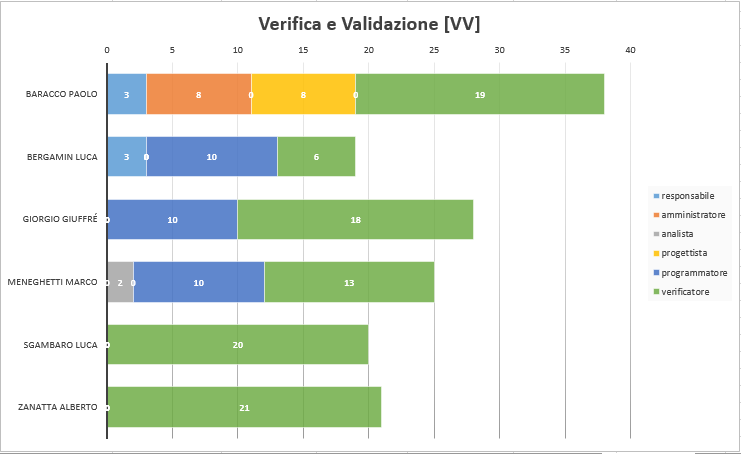
\includegraphics[width=1.1\textwidth]{img/finirevv.png}}
\caption{Ore/ruolo per persona durante la \VV.}
\label{fig:vv1}

\end{figure}

\begin{figure}[H]
\makebox[\textwidth][c]{
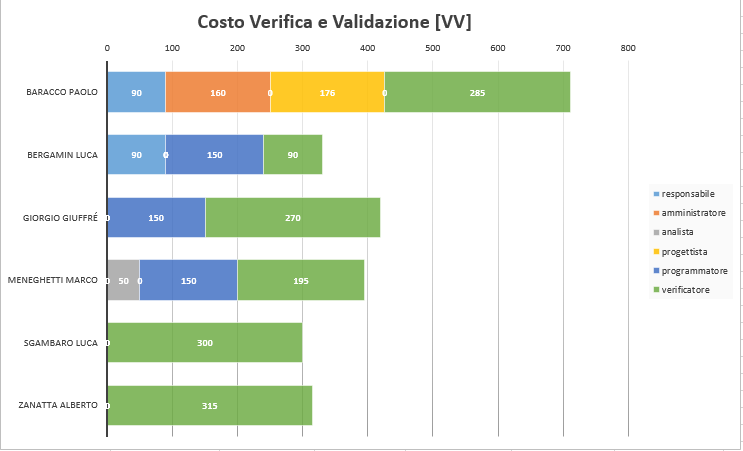
\includegraphics[width=1.1\textwidth]{img/finirevv2.png}}
\caption{Ore/persona per ruolo durante la \VV.}
\label{fig:vv2}

\end{figure}

\begin{figure}[H]
\makebox[\textwidth][c]
{
\definecolor{white2}{rgb}{0.95,0.95,0.95}
\definecolor{white3}{rgb}{0.9,0.9,0.9}
%\rowcolors{1}{white}{white2}

  \begin{tabular}{ | l | c | c | c | c | c | c | r |}
    \hline
    \rowcolor[gray]{.9}
    Ruolo / persona & \R & \AM & \AN & \PJ & \PG & \V & Tot euro/persona \\ \hline
    \PB & 90 & 160 & 0 & 176 (+176) & 0 & 285 (+210) & 711 (+386) \\ \hline
    \LB & 90 & 0 & 0 & 0 & 150 (+150) & 90 (+60) & 330 (+210) \\ \hline
    \GG & 0 & 0 & 0 & 0 &  150 (+150)  & 270 (+60) & 420 (+210) \\ \hline
    \MM & 0 & 0 & 50 & 0 &  150 (+150)  & 195 (-30) & 395 (+120) \\ \hline
    \LS & 0 & 0 & 0 & 0 & 0 & 300 (+270) & 300 (+270) \\ \hline
    \AZ & 0 & 0 & 0 & 0 & 0 & 315 (+270) & 315 (+270) \\ \hline
    \rowcolor[gray]{.9}

    Totale euro/ruolo & 180 & 160 & 50 & 176 (+176) & 450 (+450) & 1455 (+840) & 2471 (+1466) \\ \hline
  \end{tabular}
  
}\label{tab:vv}

  \caption{Tabella costo {\VV} per ruolo e per persona, valori in euro (\euro).}
\end{figure}


\subsubsection{Preventivo a finire}
Si riporta il nuovo preventivo per le ore rendicontate.

%grafici del rendicontabili e tabelle varie, far vedere come sono cambiati i costi
Successivamente sono evidenziate graficamente la divisione delle ore per persona e ruolo.

Questo quadro riassuntivo esclude il periodo di {\AR}: il totale risultante \textbf{è a carico del cliente}.

Il quantitativo rendicontato a preventivo a persona è di \textbf{104 ore} e il quantitativo di ore preventivate totali è fissato a \textbf{624 ore}.

\begin{figure}[H]
\definecolor{white2}{rgb}{0.95,0.95,0.95}
\definecolor{white3}{rgb}{0.9,0.9,0.9}
%\rowcolors{1}{white}{white2}

\makebox[\textwidth][c]
{
  \begin{tabular}[width=1.2\textwidth]{ | l | c | c | c | c | c | c | r |}
    \hline
    \rowcolor[gray]{.9}
    Ruolo / persona & \R & \AM & \AN & \PJ & \PG & \V & Tot ore/persona \\ \hline
    \PB & 3 & 8 & 0 & 34 (-10) & 27 (-3) & 32 (+14) & 104 (+1) \\ \hline
    \LB & 3 & 8 & 0 & 38 (-8) & 37 (+7) & 18 (+2) & 104 (+1) \\ \hline
    \GG & 3 & 5 & 0 & 35 (-10) & 37 (+7) & 24 (+4) & 104 (+1) \\ \hline
    \MM & 2 & 0 & 2 & 39 (-3) &  37 (+7) & 24 (-3) & 104 (+1) \\ \hline
    \LS & 2 & 3 & 5 & 28 (-18) & 27 (-3) & 39 (+22) & 104 (+1) \\ \hline
    \AZ & 2 & 5 & 8 & 23 (-18) & 27 (-3) & 39 (+22) & 104 (+1) \\ \hline
    \rowcolor[gray]{.9}

    Totale ore/ruolo & 15 & 29 & 15 & 197 (-67) & 192 (+12) & 176 (+51) & 624 (+6) \\ \hline
    
  \end{tabular}
  }
  
  \label{tab:rend}

  \caption{Tabella costo generale per ruolo e per persona, valori in euro (\euro).}
\end{figure} 
% i colori danno problemi di visualizzazione alle linee


\subsubsection{Costo ore rendicontate del progetto}
Di seguito si riporta il costo delle ore totali rendicontate, suddiviso per persona e ruolo.

Questo quadro riassuntivo esclude il periodo di {\AR}: i costi che seguono \textbf{ sono a carico del cliente}.

\begin{figure}[H]
\makebox[\textwidth][c]
{
\definecolor{white2}{rgb}{0.95,0.95,0.95}
\definecolor{white3}{rgb}{0.9,0.9,0.9}
%\rowcolors{1}{white}{white2}

  \begin{tabular}{ | l | c | c | c | c | c | c | r |}
    \hline
    \rowcolor[gray]{.9}
    Ruolo / persona & \R & \AM & \AN & \PJ & \PG & \V & Tot euro/persona \\ \hline
    \PB & 90 & 160 & 0 & 748 (-220) & 405 (-45) & 480 (+210) & 1883 (-55) \\ \hline
    \LB & 90 & 160 & 0 & 836 (-176) & 555 (+105) & 270 (+30) & 1911 (-41) \\ \hline
    \GG & 90 & 100 & 0 & 770 (-220) &  555 (+105) & 360 (+60) & 1875 (-55) \\ \hline
    \MM & 60 & 0 & 50 & 858 (-66) &  555 (+105) & 360 (-45) & 1883 (-6) \\ \hline
    \LS & 60 & 60 & 125 & 616 (-396) & 405 (-45) & 585 (+330) & 1851 (-111) \\ \hline
    \AZ & 60 & 100 & 200 & 506 (-396) & 405 (-45) & 585 (+330) & 1856 (-111) \\ \hline
    \rowcolor[gray]{.9}

    Totale euro/ruolo & 450 & 580 & 375 & 4334 (-1474) & 2880 (+180) & 2640 (+915) & 11259 (-379) \\ \hline
  \end{tabular}
  
}\label{tab:cgen}

  \caption{Tabella costo totale per ruolo e per persona, valori in euro (\euro).}
\end{figure}

Il costo totale del progetto \proj{} preventivato è pari a \textbf{11259{\euro}} (\emph{undicimilaeduecentocinquantanove euro}).


\begin{figure}[H]
\makebox[\textwidth][c]{
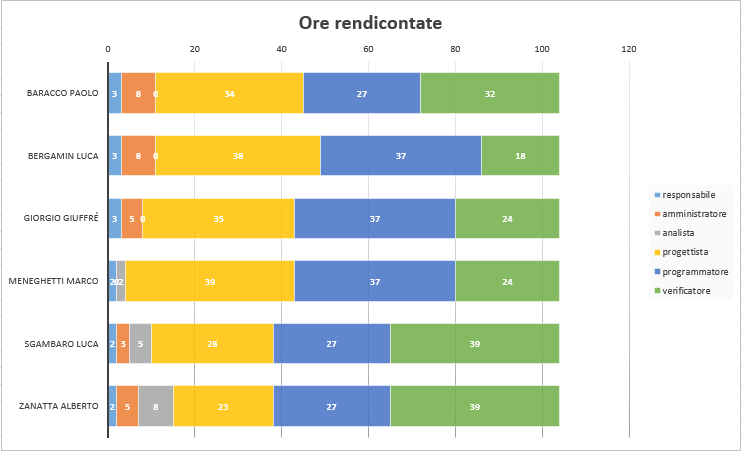
\includegraphics[width=1.2\textwidth]{img/nuovopreventivo.png}}
\label{tab:cgen1}

  \caption{Ore totali per il progetto \proj{} per persona, valori in ore.}
\end{figure}



\begin{figure}[H]
\makebox[\textwidth][c]{
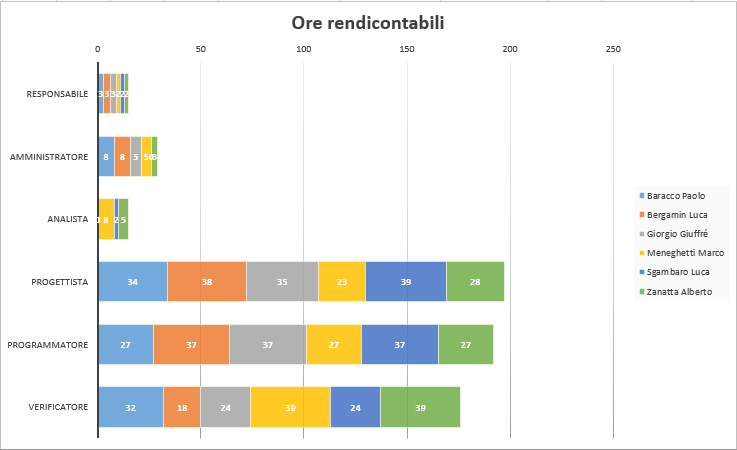
\includegraphics[width=1.2\textwidth]{img/nuovopreventivo2.png}}
\label{tab:cgen1}

  \caption{Costo totale per il progetto \proj{} per ruolo e per persona, valori in euro (\euro).}
\end{figure}




%%%%%%%%%%%%%%%%%%%%%%%%%%%%%%%%%%%%%%%%%%%%%%%%%%%%%%%%%%%%%%%%%%%%%%%%%%%%%%%%%%%%%%%%%%%%%%%%%
\pagebreak
\subsection{Consuntivo \VV}
\introconsuntivo{\VV}

\subsubsection{Variazioni nella pianificazione}

Non sono risultati ritardi nell'attuazione delle attività preventivate.

Al fine di conseguire il miglior risultato possibile, il team ha deciso di utilizzare ulteriori ore (6) per permettere una migliore riuscita delle attività di verifica, portando dunque il totale di ore rendicontate a 105 ore per ogni componente del gruppo.

\pagebreak
\subsubsection{Variazione nei costi}
\begin{itemize}

\item Sono state rilevate variazioni nei costi.

\item Si riportano le tabelle di divisione oraria effettive e i relativi costi. \textbf{Nota}: le variazioni tra parentesi si riferiscono all'ultimo preventivo a finire presentato.

\end{itemize}

\begin{figure}[H]
\definecolor{white2}{rgb}{0.95,0.95,0.95}
\definecolor{white3}{rgb}{0.9,0.9,0.9}
%\rowcolors{1}{white}{white2}

\makebox[\textwidth][c]
{
  \begin{tabular}{ | l | c | c | c | c | c | c | r |}
    \hline
    \rowcolor[gray]{.9}
    Ruolo / persona & \R & \AM & \AN & \PJ & \PG & \V & Tot ore/persona \\ \hline
    \PB & 3 & 8 & 0 & 8 & 0 & 20 (+1)& 39 (+1) \\ \hline
    \LB & 3 & 0 & 0 & 0 & 10 & 7 (+1) & 20 (+1) \\ \hline
    \GG & 0 & 0 & 0 & 0 & 10 & 19 (+1) & 29 (+1) \\ \hline
    \MM & 0 & 0 & 2 & 0 & 10 & 14 (+1) & 26 (+1) \\ \hline
    \LS & 0 & 0 & 0 & 0 & 0 & 21 (+1) & 21 (+1) \\ \hline
    \AZ & 0 & 0 & 0 & 0 & 0 & 21 (+1) & 21 (+1) \\ \hline
    \rowcolor[gray]{.9}

    Totale ore/ruolo & 6 & 8 & 2 & 8 & 30 & 102 (+6) & 156 (+6) \\ \hline
    
  \end{tabular}
  }
    \caption{Ore/ruolo per persona durante la \VV.}

\end{figure} 
% i colori danno problemi di visualizzazione alle linee

\begin{figure}[H]
\makebox[\textwidth][c]
{
\definecolor{white2}{rgb}{0.95,0.95,0.95}
\definecolor{white3}{rgb}{0.9,0.9,0.9}
%\rowcolors{1}{white}{white2}

  \begin{tabular}{ | l | c | c | c | c | c | c | r |}
    \hline
    \rowcolor[gray]{.9}
    Ruolo / persona & \R & \AM & \AN & \PJ & \PG & \V & Tot euro/persona \\ \hline
    \PB & 90 & 160 & 0 & 176 & 0 & 300 (+15) & 726 (+15) \\ \hline
    \LB & 90 & 0 & 0 & 0 & 150 & 105 (+15) & 345 (+15) \\ \hline
    \GG & 0 & 0 & 0 & 0 & 150 & 285 (+15) & 435 (+15)\\ \hline
    \MM & 0 & 0 & 50 & 0 & 150 & 210 (+15) & 410 (+15) \\ \hline
    \LS & 0 & 0 & 0 & 0 & 0 & 315 (+15) & 315 (+15) \\ \hline
    \AZ & 0 & 0 & 0 & 0 & 0 & 315 (+15) & 315 (+15) \\ \hline
    \rowcolor[gray]{.9}

    Totale euro/ruolo & 180 & 160 & 50 & 176 & 450 & 1530 (+150) & 2546 (+150) \\ \hline
  \end{tabular}
  
}\label{tab:cpdc}

  \caption{Tabella costo {\VV} per ruolo e per persona, valori in euro (\euro).}
\end{figure}


%%%% DA FARE ANCORA (so' stanco)
\begin{figure}[H]
\makebox[\textwidth][c]
{
\definecolor{white2}{rgb}{0.95,0.95,0.95}
\definecolor{white3}{rgb}{0.9,0.9,0.9}
%\rowcolors{1}{white}{white2}

  \begin{tabular}{ | l | c | r |}
    \hline
    \rowcolor[gray]{.9}
    Ruolo  & Ore & Costo \\ \hline
    \V & 156 (+6) & 2546 (+150) \\ \hline
    \rowcolor[gray]{.9}

   Differenza & +6 & +150 \\ \hline
  \end{tabular}
  
}

\label{tab:car}
\caption{Differenza preventivo-consuntivo per ruolo, \PDC. Colonna \emph{Costo} in euro (\euro).}
\end{figure}

\subsubsection{Considerazioni}

Il nuovo preventivo a finire precedentemente presentato è stato rispettato in pieno: al fine di conseguire la maggior qualità possibile con le risorse a disposizione è stato deciso di incrementate di 6 ore le attività preventivate per la verifica.

A seguito della riunione esterna del 04-05-2017, nel quale è stato presentato il lavoro fino ad allora svolto, il team è riuscito a presentare un prodotto che è riuscito a soddisfare appieno le richieste e i desideri del cliente. Sono stati raccolti consigli su come raffinare il prodotto finale sfruttando il budget aumentato per le ore di \Vx.

\pagebreak
\subsection{Consuntivo finale}

Si riporta il consuntivo dell'intero sviluppo del progetto delle sole ore rendicontate (dunque, \textbf{a carico del cliente}).

Sono indicate di seguito l'effettivo lavoro svolto complessivo in ore e tra parentesi quanto esse sono scostate dal preventivo iniziale.

Il quantitativo rendicontato a consuntivo a persona è di \textbf{105 ore} e il quantitativo di ore a consuntivo totali è fissato a \textbf{630 ore}.

\begin{figure}[H]
\definecolor{white2}{rgb}{0.95,0.95,0.95}
\definecolor{white3}{rgb}{0.9,0.9,0.9}
%\rowcolors{1}{white}{white2}

\makebox[\textwidth][c]
{
  \begin{tabular}[width=1.2\textwidth]{ | l | c | c | c | c | c | c | r |}
    \hline
    \rowcolor[gray]{.9}
    Ruolo / persona & \R & \AM & \AN & \PJ & \PG & \V & Tot ore/persona \\ \hline
    \PB & 3 & 8 & 0 & 34 (-10) & 27 (-3) & 32 (+14) & 105 (+2) \\ \hline
    \LB & 3 & 8 & 0 & 38 (-8) & 37 (+7) & 18 (+2) & 105 (+2) \\ \hline
    \GG & 3 & 5 & 0 & 35 (-10) & 37 (+7) & 24 (+4) & 105 (+2) \\ \hline
    \MM & 2 & 0 & 2 & 39 (-3) &  37 (+7) & 24 (-3) & 105 (+2) \\ \hline
    \LS & 2 & 3 & 5 & 28 (-18) & 27 (-3) & 39 (+22) & 105 (+2) \\ \hline
    \AZ & 2 & 5 & 8 & 23 (-18) & 27 (-3) & 39 (+22) & 105 (+2) \\ \hline
    \rowcolor[gray]{.9}

    Totale ore/ruolo & 15 & 29 & 15 & 197 (-67) & 192 (+12) & 182 (+67) & 630 (+12) \\ \hline
    
  \end{tabular}
  }
  
  \label{tab:rend}

  \caption{Tabella costo generale a consuntivo per ruolo e per persona, valori in euro (\euro).}
\end{figure} 

\subsubsection{Costo ore rendicontate del progetto a consuntivo}

Di seguito si riporta il costo delle ore totali rendicontate, suddiviso per persona e ruolo.

Questo quadro riassuntivo esclude il periodo di \AR{}: i costi che seguono \textbf{sono a carico del cliente}.



\begin{figure}[H]
\makebox[\textwidth][c]
{
\definecolor{white2}{rgb}{0.95,0.95,0.95}
\definecolor{white3}{rgb}{0.9,0.9,0.9}
%\rowcolors{1}{white}{white2}

  \begin{tabular}{ | l | c | c | c | c | c | c | r |}
    \hline
    \rowcolor[gray]{.9}
    Ruolo / persona & \R & \AM & \AN & \PJ & \PG & \V & Tot euro/persona \\ \hline
    \PB & 90 & 160 & 0 & 748 (-220) & 405 (-45) & 495 (+225) & 1898 (-40) \\ \hline
    \LB & 90 & 160 & 0 & 836 (-176) & 555 (+105) & 285 (+45) & 1926 (-26) \\ \hline
    \GG & 90 & 100 & 0 & 770 (-220) &  555 (+105) & 375 (+75) & 1890 (-40) \\ \hline
    \MM & 60 & 0 & 50 & 858 (-66) &  555 (+105) & 375 (-30) & 1898 (+9) \\ \hline
    \LS & 60 & 60 & 125 & 616 (-396) & 405 (-45) & 600 (+345) & 1866 (-96) \\ \hline
    \AZ & 60 & 100 & 200 & 506 (-396) & 405 (-45) & 600 (+345) & 1871 (-96) \\ \hline
    \rowcolor[gray]{.9}

    Totale euro/ruolo & 450 & 580 & 375 & 4334 (-1474) & 2880 (+180) & 2640 (+915) & 11349 (-289) \\ \hline
  \end{tabular}
  
}\label{tab:cgen}
\end{figure}
\pagebreak
\subsection{Considerazioni finali}
\subsubsection{Aumento attività verifica}
Il presente \emph{Piano di Progetto} ha ricevuto vari incrementi nel tempo, ma la modifica più critica è stata la riassegnazione di parte delle risorse alle attività di verifica, sottraendole alle attività preventivate di progettazione.

Questa scelta è risultata soddisfacente per l'attività del team: attraverso varie riunioni con il proponente è stato possibile trovare un punto d'incontro che ci ha permesso di ridurre le richieste progettuali e concentrarci nel conseguimento degli obiettivi posti nel \emph{Piano di Qualifica}.

\subsubsection{Pianificazione di \PDC e \VV}
La pianificazione di queste due fasi ha ricevuto una sostanziale modifica, come già indicato nel consuntivo di periodo rispettivo.

Al termine del progetto, possiamo concludere che la \VV non ne abbia risentito: le attività preventivate sono state svolte senza ritardi ed è stato possibile consegnare il prodotto in tempo. 
 
\subsubsection{Specializzazione dei componenti del team}
È stato possibile notare durante l'individuazione e assegnazione delle sotto-attività necessarie a completare le attività principali (visualizzate nel presente \emph{Piano di Progetto} tramite diagrammi di Gantt) come i singoli membri del team si siano \textbf{specializzati} in una o più mansioni. Questo è stato di grande aiuto:

\begin{itemize}
\item la presenza di un membro del gruppo più informato in un ruolo ha permesso di istruire efficacemente gli altri componenti durante i cambi di ruolo;
\item questa figura si traduce in una figura "senior": questa può supervisionare il lavoro degli altri componenti, riferire l'andamento delle attività al \Rx, comprendere più in profondità le criticità da risolvere.
\end{itemize} 

Tuttavia la specializzazione dei membri del gruppo avviene ad un prezzo: un maggior costo in ore. È stato dunque necessario ridistribuire le ore assegnate per i componenti al fine di possedere una rendicontazione fedele a quanto avvenuto.

Di seguito si indicano i ruoli assunti maggiormente dai componenti del gruppo, qualora non fosse già chiara dal consuntivo indicato in precedenza; tuttavia ciò non implica che ogni componente non abbia avuto la possibilità di cimentarsi in ogni ruolo del progetto.

\begin{itemize}
\item[\PB] \ANx{};
\item[\LB] \Rx{}, \PGx{};
\item[\GG] \AMx{}, \Vx{}, \PGx{};
\item[\MM] \PJx{}, \PGx{};
\item[\LS] \Vx{};
\item[\AZ] \Vx{};
\end{itemize}

\pagebreak
\subsubsection{Costo totale}
Il costo totale \textbf{a carico del cliente} è pari a \textbf{11349\euro} (\textit{undicimilatrecentoquarantanove euro}).

Questo costo differisce per una cifra negativa (-289\euro) rispetto a quanto preventivato. Ciò è imputabile alla riassegnazione oraria delle attività: sottraendo ore alle attività di progettazione e aggiungendone in egual misura alle attività di verifica risulta un risparmio del 20\% a causa dei differenti costi dei due ruoli. Sono state investite maggiori risorse nelle attività di codifica fino al raggiungimento delle 105 ore/persona massime consentite.


%%%%%%%%%%%%%%%%%%%%%%%%%%%%%%%%%%%%%%%%%%%%%%%%%%%%%%%%%%%%%%%%%%%%%%%%%%


%%%%%%%%%%%%%%%%
%%  Organigramma
%%%%%%%%%%%%%%%%

\section{Organigramma}	\label{sec:organigramma}
\subsection{Redazione}

\begin{figure}[H]
\makebox[\textwidth][c]
{
  \begin{tabular}{ | c | c | c |}
			\hline
			\textbf{Nominativo} & \textbf{Data di redazione} & \textbf{Firma} \\
			\hline
			\LB & 25-12-2016 &   \myincludegraphics{img/firmalb.jpg}\\
			\hline
  \end{tabular}
}
\caption{Redazione}
\end{figure}

\subsection{Approvazione}
\begin{figure}[H]
\makebox[\textwidth][c]
{
  \begin{tabular}{ | c | c | c |}
			\hline
			\textbf{Nominativo}     & \textbf{Data di approvazione} & \textbf{Firma}  \\
			\hline
			\LB		& 24-01-2017	&  \myincludegraphics{img/firmalb.jpg}	\\
			\hline
			\TV	          &		           &			\\
			\hline
\end{tabular}
}
\caption{Approvazione}
\end{figure}

\subsection{Accettazione dei componenti}
\begin{figure}[H]
\makebox[\textwidth][c]
{
  \begin{tabular}{ | c | c | c |}
			\hline
			\textbf{Nominativo} & \textbf{Data} & \textbf{Firma} \\
			\hline
			\AZ		&	24-01-2017	&  \myincludegraphics{img/firmaaz.jpg}	\\
			\hline
			\GG		&	24-01-2017   &  \myincludegraphics[scale=0.75]{img/firmagg.png}	\\
			\hline
			\LB		&	24-01-2017	&  \myincludegraphics{img/firmalb.jpg}		\\
			\hline
			\LS		&	24-01-2017	&  \myincludegraphics{img/firmals.jpg}		\\
			\hline
			\MM		&	24-01-2017	&  \myincludegraphics{img/firmamm.png}		\\
			\hline
			\PB		&	24-01-2017	&  \myincludegraphics{img/firmapb.png}		\\
			\hline
\end{tabular}
}
\caption{Accettazione}
\end{figure}

\subsection{Componenti}
\begin{figure}[H]
\makebox[\textwidth][c]
{
  \begin{tabular}{ | c | c | c | c |}
			\hline
			\textbf{Nominativo} & \textbf{Matricola} & \raggedright \textbf{Indirizzo di posta elettronica} & \textbf{Ruoli} \\[1ex]
			\hline
	 		\AZ	& 1100543	& \href{mailto:alberto.zanatta.3@studenti.unipd.it}{alberto.zanatta.3@studenti.unipd.it} 	& \AN,  \V	\\[1ex]
			\hline
			\GG		& 1069456	& \href{mailto:giorgio.giuffre@studenti.unipd.it}{giorgio.giuffre@studenti.unipd.it} 	&  \AN, \AM, \V	\\[1ex]
			\hline
			\LB		& 1097055	& \href{mailto:luca.bergamin.3@studenti.unipd.it}{luca.bergamin.3@studenti.unipd.it}  &  \AN, \R, \V \\[1ex]
			\hline
			\LS 		& 1099154	& \href{mailto:luca.sgambaro@studenti.unipd.it}{luca.sgambaro@studenti.unipd.it} 	& \AN, \V	\\[1ex]
			\hline
			\MM		& 1097051	& \href{mailto:marco.meneghetti.5@studenti.unipd.it}{marco.meneghetti.5@studenti.unipd.it} & \AN, \AM, \V	\\[1ex]
			\hline
			\PB		& 1097928	& \href{mailto:paolo.baracco.1@studenti.unipd.it}{paolo.baracco.1@studenti.unipd.it} 	&  \AN, \R, \V 	\\[1ex]
			\hline
\end{tabular}
}
\caption{Componenti}
\end{figure}





\appendix

%%%%%%%%%%%%%%%%%%%%%%%
%%  Modelli di sviluppo
%%%%%%%%%%%%%%%%%%%%%%%

\section{Modelli di sviluppo} \label{sec:modelli}

Di seguito vengono analizzati sinteticamente punti deboli e punti di forza dei principali approcci ai processi software, nel contesto del nostro progetto.

Va tuttavia ricordato che non è sconsigliato adottare più modelli in forma ibrida, come suggerito da Sommerville (vedi \ref{sec:ref}).

\subsection{Modelli di sviluppo sequenziali}

\subsubsection{Modello a cascata}
Il modello a cascata (Royce, 1970) è il più antico dei modelli software analizzati e fondamentalmente identifica cinque attività di sviluppo principali:
\begin{description}
	\item [Analisi e definizione dei requisiti] il problema viene ben definito, specificando obiettivi e vincoli;
	\item [Progettazione del sistema] si stabilisce un'architettura software;
	\item [Implementazione e test di unità] sono sviluppate una serie di unità e i loro relativi test;
	\item [Integrazione e test di sistema] le singole unità sono integrate e sono effettuati test di sistema che devono soddisfare le specifiche iniziali;
	\item [Manuntenzione] la fase del ciclo di vita auspicabilmente più longeva.
\end{description}

Questo tipo di approccio:
\begin{itemize}
	\item promette un prodotto finito, con grande attenzione alle deadline tracciate inizialmente;
	\item stabilisce una architettura software iniziale stabile.
\end{itemize}

Di contro, i svantaggi di questo approccio sono svariati:
\begin{itemize}
	\item le varie fasi sono a compartimenti stagni --- una volta tracciati i requisiti, essi non possono più venire modificati;
	\item il committente deve avere già inizialmente una idea molto chiara del prodotto che desidera.
\end{itemize}
Questi ultimi punti entrano in netto contrasto con i requisiti inizialmente proposti; ciò ha portato a scartare questo modello di sviluppo. Tuttavia adottiamo una politica a \emph{deadline}, anche a causa dei vincoli imposti dalle revisioni del \TV.

\subsubsection{Modello evolutivo}
Il modello evolutivo, particolarmente apprezzato da Sommerville, prevede una implementazione iniziale e una forte collaborazione tra committente e fornitore allo scopo di raffinare il sistema tramite più versioni del prodotto, fino a raggiungere un sistema adeguato alle esigenze dell'utente.

Ciò si può realizzare principalmente tramite due strumenti differenti: lo \emph{exploratory development} e il \emph{throwaway prototyping}.

Il primo consiste nel lavorare a fianco del cliente per esplorare i suoi requisiti e infine consegnare un sistema adeguato. Benché questo metodo di lavoro potrebbe sembrare positivo, esso presenta due grosse criticità: 
\begin{itemize}
	\item cambiamenti continui tendono a corrompere la struttura e l'architettura del software;
	\item aggiungere estensioni non previste diventa progressivamente più complesso e costoso. 
\end{itemize}
Questo rischio a parere di \hx{} non riesce ad essere bilanciato dalla possibilità di ritardare requisiti e decisioni di design.

La seconda possibilità invece consiste nell'avere dei prototipi usati per meglio comprendere il problema. La criticità presente riguarda il futuro di questi prototipi: sviluppare un prototipo porta valore esclusivamente nell'ambito di comprensione dei requisiti del progetto; non porta un effettivo avanzamento nello sviluppo del prodotto.

\subsubsection{Modello basato su componenti}
Questo modello si basa sull'approccio orientato al riuso di componenti già esistenti, in modo da abbattere tempi e costi. Esso si differenzia per alcuni differenti fasi intermedie orientate al riuso:
\begin{description}
	\item [Analisi delle componenti] a partire dalla specifica dei requisiti, sono ricercati delle componenti già esistenti che possano soddisfare la specifica esistente.
	\item [Modifica dei requisiti] i requisiti variano a seconda delle componenti che sono state identificate.
	\item [Progettazione del sistema con riuso] viene tracciata l'architettura del sistema e sono progettate in dettaglio le componenti non disponibili al riuso.
	\item [Sviluppo e integrazione] Sono sviluppate le componenti non esistenti ed esse sono integrate al sistema con riuso. L'integrazione e lo sviluppo possono non essere attività separate.
\end{description}

Questo approccio è sicuramente interessante e, malgrado non sia stato adottato in toto, ci si riserva la possibilità di seguire i punti che prevedono il design del sistema con riuso e una modifica dei requisiti, al fine di ridurre i tempi e costi di certe componenti del sistema. \hx{} ritiene inoltre che gli svantaggi riguardo ai compromessi che nasceranno siano di gran lunga ripagati dai benefici di questo approccio; infine l'approccio è stato approvato dal committente in sede di discussione.

\subsection{Modelli di sviluppo iterativi}

\subsubsection{Modello incrementale}
Questo modello sfrutta un approccio che vuole combinare i vantaggi del modello a cascata con il modello evolutivo. Essenzialmente si prevede che il committente identifichi le componenti più importanti e meno importanti; quindi si sviluppa una architettura di base e si fissano degli incrementi delle funzionalità del sistema in iterazioni successive.

Questo modello richiede che ogni incremento:
\begin{itemize}
	\item Apporti funzionalità tangibili;
	\item Non deve essere eccessivamente ampio (<20mila righe di codice)
	\item Sia validato singolarmente, integrato e sia validato nel complesso
\end{itemize}

I vantaggi di questo modello sono molteplici:
\begin{itemize}
	\item Permette di sperimentare il sistema con il committente al fine di chiarificare tutti i requisiti;
	\item I primi incrementi possono essere usati come prototipi;
	\item I servizi a più alta priorità passano inevitabilmente il maggior numero di fasi di test.
\end{itemize}

Vanno segnalati tuttavia i seguenti difetti:
\begin{itemize}
\item Può essere difficile trasformare i requisiti del cliente in incrementi di una misura adeguata;
\item Non è possibile modificare i requisiti già esistenti negli incrementi successivi.
\end{itemize}
Ciò si traduce in una criticità del processo nella fase di analisi. Nella sezione {\ref{sec:rischi}} (Analisi dei rischi) si analizza come questo rischio verrà trattato.

In complesso, \hx{} ritiene che il modello incrementale apporti sostanziali vantaggi rispetto agli altri modelli finora analizzati. In seguito si analizzano altri modelli che sono stati presi in considerazione.

\subsubsection{Modello a spirale}
Il modello a spirale (Boehm, 1988) è un approccio fondamentalmente rappresentato come una sequenza di attività che si ripetono nel tempo, partendo dalla fattibilità, definizione dei requisiti, ideazione dell'architettura, e così via. Le quattro operazioni ripetute all'interno della spirale sono:
\begin{itemize}
	\item Identificazione degli obiettivi
	\item Valutazione del rischio
	\item Sviluppo e validazione
	\item Pianificazione (della fase successiva)
\end{itemize}			 

L'approccio sfrutta una metodologia fortemente \emph{risk-driven} che, malgrado possa portare dei benefici al prodotto finale, rischierebbe di appesantire eccessivamente il team, il processo di sviluppo e le risorse.



\end{document}
